\documentclass[12pt,a4paper]{report}

\usepackage[utf8]{inputenc} % pentru suport diacritice
\usepackage[romanian]{babel} % setări pentru limba română 
\usepackage{sansmathfonts}
\renewcommand\familydefault{\sfdefault} % sans serif
\DeclareFontSeriesDefault[sf]{bf}{bx}

\usepackage[margin=2.54cm]{geometry}	% dimensiuni pagină și margini
\usepackage{graphicx} % support the \includegraphics command and options
\usepackage{subcaption} % for subfigures
\usepackage{algorithm}
\usepackage{algpseudocode}
\usepackage{xpatch}

% formatting sections and subsections
\usepackage{textcase}
\usepackage[titletoc, title]{appendix}
\usepackage{titlesec}
\titleformat{\chapter}{\large\bfseries\MakeUppercase}{\thechapter}{2ex}{}[\vspace*{-1.5cm}]
\titleformat*{\section}{\large\bfseries}
\titleformat*{\subsection}{\large\bfseries}
\titleformat*{\subsubsection}{\large\bfseries}

\usepackage{chngcntr}
\counterwithout{figure}{chapter} % no chapter number in figure labels
\counterwithout{table}{chapter} % no chapter number in table labels
\counterwithout{equation}{chapter} % no chapter number in equation labels

\usepackage{booktabs} % for much better looking tables
\usepackage{url} % Useful for inserting web links nicely
\urlstyle{same}	% same font as regular text
\usepackage{scrextend} % for multiple footnote references
\usepackage{fnpct} % for multiple footnotes in the same place
\usepackage[bookmarks,unicode,hidelinks]{hyperref}

\usepackage{array} % for better arrays (eg matrices) in maths
\usepackage{paralist} % very flexible & customisable lists (eg. enumerate/itemize, etc.)
\usepackage{verbatim} % adds environment for commenting out blocks of text & for better verbatim
\usepackage{enumitem}
\setlist{noitemsep}

\usepackage{xurl} % for breaking long URLs
\usepackage{amsmath}
\usepackage{amssymb} % for math symbols
\usepackage{pgfplots}
\pgfplotsset{compat=1.18}

\usepackage[section]{placeins}
\usepackage{listings}
\usepackage{xcolor}

\definecolor{codegreen}{rgb}{0,0.6,0}
\definecolor{codegray}{rgb}{0.5,0.5,0.5}
\definecolor{codepurple}{rgb}{0.58,0,0.82}
\definecolor{backcolour}{rgb}{0.95,0.95,0.92}

\lstdefinestyle{mystyle}{
    backgroundcolor=\color{backcolour},   
    commentstyle=\color{codegreen},
    keywordstyle=\color{magenta},
    numberstyle=\tiny\color{codegray},
    stringstyle=\color{codepurple},
    basicstyle=\ttfamily\scriptsize,
    breakatwhitespace=false,         
    breaklines=true,                 
    captionpos=b,                    
    keepspaces=true,                 
    numbers=left,                    
    numbersep=5pt,                  
    showspaces=false,                
    showstringspaces=false,
    showtabs=false,                  
    tabsize=2
}
\lstset{style=mystyle}
\renewcommand{\lstlistingname}{Listarea}

% for integrals
\newcommand*\diff{\mathop{}\!\mathrm{d}}
\newcommand*\Diff[1]{\mathop{}\!\mathrm{d^#1}}

% rename Algorithm to Algoritm
\floatname{algorithm}{Algoritmul}

% change algorithmic font
\xpatchcmd{\algorithmic}{\setcounter}{\algorithmicfont\setcounter}{}{}
\providecommand{\algorithmicfont}{}
\providecommand{\setalgorithmicfont}[1]{\renewcommand{\algorithmicfont}{#1}}
% \renewcommand{\algorithmiccomment}[1]{{\small\hfill$\triangleright$ #1}}
\setalgorithmicfont{\footnotesize}

\usepackage{amsthm}
\newtheorem{definition}{Definiția}

\captionsetup{font=small,width=0.8\textwidth}


%%% HEADERS & FOOTERS
\usepackage{fancyhdr}
\pagestyle{empty}
\renewcommand{\headrulewidth}{0pt}
\renewcommand{\footrulewidth}{0pt}
\lhead{}\chead{}\rhead{}
\lfoot{}\cfoot{\thepage}\rfoot{}



\newcommand{\HeaderLineSpace}{-0.25cm}
\newcommand{\UniTextRO}{UNIVERSITATEA NAȚIONALĂ DE ȘTIINȚĂ ȘI TEHNOLOGIE \\[\HeaderLineSpace] POLITEHNICA BUCUREȘTI \\[\HeaderLineSpace] 
FACULTATEA DE AUTOMATICĂ ȘI CALCULATOARE \\[\HeaderLineSpace]
DEPARTAMENTUL DE CALCULATOARE\\}
\newcommand{\DiplomaRO}{PROIECT DE DISERTAȚIE}
\newcommand{\AdvisorRO}{Coordonator științific:}
\newcommand{\BucRO}{BUCUREȘTI}

\newcommand{\UniTextEN}{NATIONAL UNIVERSITY OF SCIENCE AND TECHNOLOGY \\[\HeaderLineSpace] POLITEHNICA BUCHAREST \\[\HeaderLineSpace]
FACULTY OF AUTOMATIC CONTROL AND COMPUTERS \\[\HeaderLineSpace]
COMPUTER SCIENCE AND ENGINEERING DEPARTMENT\\}
\newcommand{\DiplomaEN}{DISSERTATION PROJECT}
\newcommand{\AdvisorEN}{Thesis advisor:}
\newcommand{\BucEN}{BUCHAREST}

\newcommand{\frontPage}[6]{
\begin{titlepage}
\begin{center}
{\Large #1}  % header (university, faculty, department)
\vspace{50pt}
\begin{tabular}{m{6cm}m{4cm}}

\includegraphics[scale=0.11]{pics/PB_logo_ro.png} &
	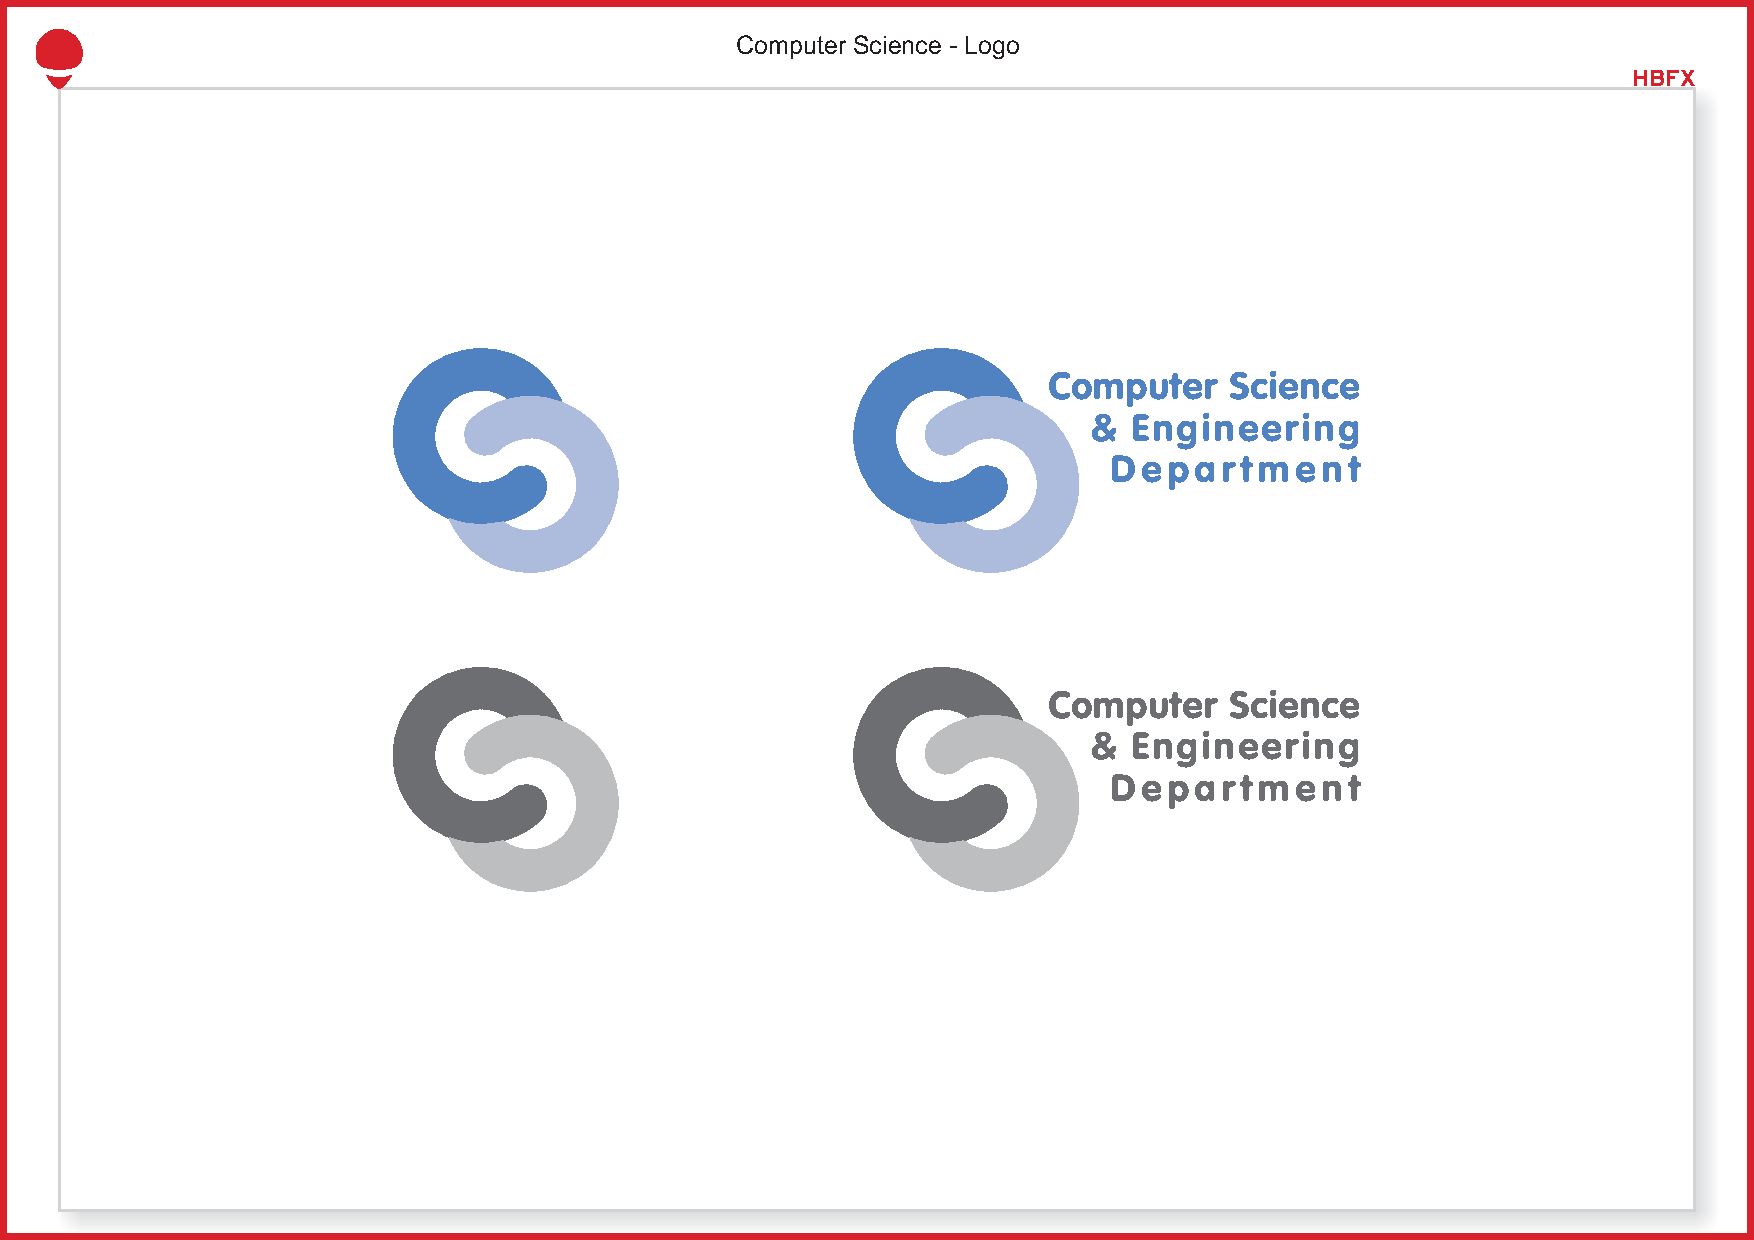
\includegraphics[scale=0.6,trim={14cm 11cm 2cm 5cm},clip=true]{pics/cs-logo.pdf} \\
\end{tabular}

\vspace{105pt}
{\Huge #2}\\                           % diploma project text
\vspace{40pt}
{\Large #3}\\ \vspace{0pt}  % project title
{\Large #4}\\                          % project subtitle
\vspace{40pt}
{\LARGE \Name}\\                   % student name
\end{center}
\vspace{60pt}
\begin{tabular*}{\textwidth}{@{\extracolsep{\fill}}p{6cm}r}
&{\large\textbf{#5}}\vspace{10pt}\\      % scientific advisor
&{\large \Advisor}                                    % advisor name
\end{tabular*}
\vspace{20pt}
\begin{center}
{\large\textbf{#6}}\\                                % bucharest
\vspace{0pt}
{\normalsize \Year}
\end{center}
\end{titlepage}
}

\newcommand{\frontPageRO}{\frontPage{\UniTextRO}{\DiplomaRO}{\ProjectTitleRO}{\ProjectSubtitleRO}{\AdvisorRO}{\BucRO}}
\newcommand{\frontPageEN}{\frontPage{\UniTextEN}{\DiplomaEN}{\ProjectTitleEN}{\ProjectSubtitleEN}{\AdvisorEN}{\BucEN}}

\linespread{1.15}
\setlength\parindent{0pt}
\setlength\parskip{.28cm}

%% Abstract macro
\newcommand{\AbstractPage}{
\begin{titlepage}
\textbf{\large SINOPSIS}\par
\AbstractRO\par\vfill
\textbf{\large ABSTRACT}\par
\AbstractEN \vfill
\end{titlepage}
}

%% Thank you macro
\newcommand{\ThanksPage}{
\begin{titlepage}
{\noindent \large\textbf{MULȚUMIRI}}\\
\Thanks
\end{titlepage}
}



%%%%%%%%%%%%%%%%%%%%%%%%%%%%%%%%%%%%%%%%%%%%%%%%%%   
%%
%%          End of template definitions
%%   
%%%%%%%%%%%%%%%%%%%%%%%%%%%%%%%%%%%%%%%%%%%%%%%%%%


%%% Puteți elimina aceste linii din lucrare, servesc numai pentru template.
\newcommand{\worktype}[1]{[\textit{#1}] }
\newcommand{\dezvoltare}{\worktype{Dezvoltare de produs}}
\newcommand{\cercetare}{\worktype{Cercetare}}
\newcommand{\ambele}{\worktype{Ambele}}
%%%


%%
%%   Campurile de mai jos trebuie modificate de autor. Modificati doar continutul, nu si numele fiecarei definitii
%%
\newcommand{\ProjectTitleRO}{Motor grafic în Vulkan}
\newcommand{\ProjectSubtitleRO}{cu pipeline de Ray Tracing}
\newcommand{\ProjectTitleEN}{Graphics engine in Vulkan}
\newcommand{\ProjectSubtitleEN}{using the Ray Tracing pipeline}
\newcommand{\Name}{Alex-Andrei Cioc}
\newcommand{\Advisor}{Conf. Dr. Ing. Victor Asavei}
\newcommand{\Year}{2026}

% Setări document
\title{Proiect de diplomă}
\author{\Name}
\date{\Year}

%%
%%   Campurile aferente rezumatului
%%
\newcommand{\AbstractRO}{
De-a lungul timpului, au fost analizate și dezvoltate numeroase tehnici de redare a imaginilor.
Tehnica Ray Tracing a fost una dintre primele tehnici de redare a imaginilor pe calculator, dar aceasta nu era considerată interactivă.
Complexitatea sa computațională notorie, cauzată de explozia recursivă a razelor aruncate în scenă, a îndreptat industria spre a adopta tehnici bazate pe rasterizare.
Jocurile video au beneficiat de pe urma acestor tehnici interactive, în timp ce Ray Tracing a fost folosit în principal în industriile de producție de filme și animație, unde fidelitatea vizuală este mai importantă decât performanța în timp real.

În 2018, NVIDIA a revoluționat industria grafică prin introducerea de hardware specializat de accelerare a Ray Tracing-ului în arhitectura Turing\footnote{\label{turing}\url{https://images.nvidia.com/aem-dam/en-zz/Solutions/design-visualization/technologies/turing-architecture/NVIDIA-Turing-Architecture-Whitepaper.pdf}. Accesat 13.06.2026.}, impunând o schimbare de paradigmă în industria grafică.
Competitorii săi, AMD și Intel, au urmat rapid, lansând propriile lor soluții de accelerare a Ray Tracing-ului.
În ziua de astăzi, majoritatea lansărilor de jocuri AAA includ suport pentru Ray Tracing\footnote{\label{raytracing-games}\url{https://www.pcgamingwiki.com/wiki/List_of_games_that_support_ray_tracing}. Accesat 13.06.2026.}, unele chiar pentru Path Tracing.

Această lucrare pleacă de la studiul desfășurat în cadrul proiectului de diplomă~\cite{DieXaR2024}, care a avut ca scop implementarea unui algoritm de Ray Tracing în timp real, folosind API-ul DirectX Raytracing.
Scopul lucrării este de a porta acest algoritm pe o platformă modernă și portabilă, folosind API-ul Vulkan, totodată aducând îmbunătățiri vizuale, de performanță, dar și de experiență a utilizatorului.
}

\newcommand{\AbstractEN}{
Throughout time, numerous image rendering techniques were analyzed and developed.
Ray Tracing was one of the first computer image rendering techniques, but it was not considered interactive.
Its notorious computational complexity, caused by the recursive explosion of rays cast into the scene, led the industry to adopt rasterization-based techniques.
Video games benefited from these interactive techniques, while Ray Tracing was used mainly in the film and animation industries, where visual fidelity is more important than real-time performance.

In 2018, NVIDIA revolutionized the graphics industry by introducing specialized Ray Tracing acceleration hardware in the Turing architecture\footref{turing}, ushering in a paradigm shift in the graphics industry.
Its competitors, AMD and Intel, quickly followed, launching their own Ray Tracing acceleration solutions.
Today, most AAA game releases include support for Ray Tracing\footref{raytracing-games}, some even for Path Tracing.

This thesis builds on the study carried out as part of the bachelor's thesis project~\cite{DieXaR2024}, whose goal was to implement a real-time Ray Tracing algorithm using the DirectX Raytracing API.
The aim of this thesis is to port that algorithm to a modern and portable platform using the Vulkan API, while also bringing visual, performance, and user experience improvements.
}



%%
%%   Campurile aferente paginii de multumiri
%%
\newcommand{\Thanks}{Adresez mulțumiri coordonatorului meu de proiect, Conf. Dr. Ing. Victor Asavei, pentru îndrumarea
și sprijinul acordat pe parcursul realizării acestei lucrări, dar și pentru
inspirația și motivația oferită în cadrul cursurilor de Motoare Grafice.
Dumnealui m-a încurajat să continui cercetarea începută în cadrul proiectului de diplomă și să o extind în această lucrare.
De asemenea, mulțumesc familiei și prietenilor pentru susținere și încurajare.}

\numberwithin{equation}{section} % for equation numbering

\begin{document}

\frontPageRO
\frontPageEN

\begingroup
\linespread{1}
\tableofcontents
\endgroup

\AbstractPage

% poate fi comentata sau stearsa
\ThanksPage


% Textul licentei incepe de aici 



\chapter{Introducere}\pagestyle{fancy}
% * <marios.choudary@gmail.com> 2018-02-28T11:38:18.106Z:
% 
% > INTRODUCERE
% Am scos de aici referintele la font pentru a nu mai fi dependenti de Calibri. Personal, nici nu sunt sigur ca ajuta prea mult aceasta recomandare si mi se pare bun font-ul default din Latex (Computer Modern). Daca sunteti de-acord, va rog sa stergeti liniile comentate de mai jos, precum si cele referitoare la fontul Calibri din restul documentului.
% 
% ^.

\section{Context}

În cadrul proiectului de diplomă~\cite{DieXaR2024}, am implementat un algoritm de Ray Tracing în timp real folosind API-ul DirectX Raytracing.
Acest proiect a fost ales ca urmare a interesului meu pentru grafica pe calculator și limitele pe care tehnologia curentă le poate atinge în ceea ce privește fidelitatea vizuală.
Deși am reușit să obțin rezultate promițătoare, implementând un algoritm de nivel cinematic și adăugând efecte vizuale precum reflexii, refracții și umbre, am întâmpinat limitări legate de performanță și portabilitate.
De asemenea, experiența utilizatorului a fost limitată -- scenele erau predefinite, obiectele și materialele nu putea fi modificate în timp real, ci necesitau recompilarea shader-elor și a codului CPU.
Arhitectura proiectului a fost rigidă, majoritatea logicii fiind implementată la un loc, fără o separare clară a responsabilităților și fără abstractizări semnificative.
Stadiul proiectului a fost, fără doar și poate, unul de prototip, de MVP (Minimum Viable Product), însă algoritmul de bază a fost implementat robust, servind drept o fundație solidă pentru a construi în jurul acestuia.

Tehnologia a avansat din 2024 încoace, iar API-ul Vulkan mi-a atras atenția ca fiind o platformă modernă și portabilă, care oferă un control mai mare asupra resurselor hardware și o performanță mai bună în anumite scenarii comparativ cu DirectX.
Opinia publică s-a schimbat spre direcția impunerii unei modernizări a API-urilor grafice, având în vedere faptul că Direct3D 12, ultima versiune majoră de la Microsoft, a fost lansată oficial în urmă cu mai bine de 10 ani, iar hardware-ul a evoluat semnificativ în acest timp.
Pe de altă parte, Vulkan beneficiază de un suport larg din partea industriei, fiind adoptat de majoritatea producătorilor de hardware și software, și oferă o platformă unificată pentru dezvoltarea de aplicații grafice pe multiple sisteme de operare și dispozitive.
Ultima versiune majoră, Vulkan 1.4, a fost lansată la scurt timp după finalizarea proiectului de diplomă și primește actualizări regulate.
De asemenea, Vulkan 1.3 (2022) a provocat o schimbare de paradigmă majoră, prin introducerea conceptului de Dynamic Rendering\footnote{\url{https://docs.vulkan.org/samples/latest/samples/extensions/dynamic_rendering/README.html}. Accesat 13.06.2026.}, care permite redarea fără a fi nevoie de crearea și gestionarea obiectelor de tip \texttt{Render Pass} și \texttt{Framebuffer}, simplificând semnificativ procesul de dezvoltare și oferind o flexibilitate crescută în ceea ce privește tehnicile de redare utilizate.

\section{Problemă abordată}

Lucrarea de față abordează, la nivel practic, problema implementării unui algoritm de Ray Tracing în timp real folosind API-ul Vulkan, împreună cu un model de iluminare compatibil PBR (Physically Based Rendering).
Problema de fond este, însă, mai largă și în esență derivată din problema abordată în proiectul de diplomă, și anume: \textit{cum putem aduce tehnici avansate de redare a imaginilor, precum Ray Tracing, pe platforme moderne și portabile, în timp ce menținem o performanță acceptabilă și o experiență plăcută pentru utilizator?}
Deși au trecut 2 ani de la finalizarea proiectului de diplomă, această problemă rămâne relevantă și provocatoare, și va rămâne așa pentru o perioadă semnificativă de timp.
Criza semiconductorilor și a lanțurilor de aprovizionare se opun avansului tehnologic, ceea ce limitează progresul cu care fidelitatea vizuală poate fi crescută.
Acest lucru motivează dezvoltatorii să găsească soluții și tehnici de optimizare pentru a reduce costurile computaționale ale algoritmilor de redare a imaginilor, pentru a putea prelungi durata de viață a hardware-ului existent, concomitent cu păstrarea progresului la nivel de fidelitate vizuală.

\section{Obiective}

Obiectivul de fond nu s-a schimbat.
Lucrarea își propune, în continuare, să implementeze un algoritm de Ray Tracing care să aducă o fidelitate vizuală ridicată, în timp real.
Fundația oferită de proiectul de diplomă reprezintă un punct de plecare solid, iar obiectivele secundare se învârt în jurul îmbunătățirilor pe multiple planuri.

Astfel, putem marca un prim obiectiv secundar: \textbf{portabilitatea}.
Proiectul de diplomă a fost implementat folosind API-ul DirectX Raytracing, care este specific platformei Microsoft Windows.
Pentru a rula \textit{nativ} pe platforme derivate din Linux (Ubuntu, Fedora, CachyOS, SteamOS, etc.), codul sursă trebuie portat pentru a folosi API-ul Vulkan, care este suportat pe o gamă largă de platforme și dispozitive.
În afară de portarea codului în sine, trebuie făcute modificări și la sistemul de build, pentru a asigura compilarea și rularea pe multiple platforme.

Un alt obiectiv important este suportul \textbf{texturilor PBR}.
Deși proiectul de diplomă a implementat un model de iluminare compatibil PBR (Disney's Principled BSDF~\cite{DisneyBSDF}), implementarea actuală nu suportă încărcarea și utilizarea texturilor de niciun fel, ci folosește doar informația albedo pentru a determina culoarea de bază a materialelor.
Adăugând suport pentru definirea și încărcarea texturilor precum \texttt{albedo}, \texttt{normal map}, \texttt{roughness}, \texttt{metallic}, etc., putem aduce un plus semnificativ de realism vizual și diversitate în scenele generate.
Suprafețele pot avea detalii variate, pot avea proprietăți diferite de-a lungul lor, și pot interacționa cu lumina într-un mod mult mai complex și realist.

Din sfera de \textit{featurefulness}, un alt obiectiv este suportul pentru \textbf{definire, încărcare, modificare și salvare a scenelor}.
Pentru a fi cu adevărat util, motorul grafic trebuie să suporte încărcarea scenelor de pe disc, precum și modificarea acestora în timp real, fără a fi nevoie de recompilarea shader-elor sau a codului CPU.
Acest aspect include suportul pentru formate de fișiere comune, cum ar fi \texttt{glTF}, care pot conține informații despre geometrie, materiale, texturi, lumină și alte atribute ale scenei.

Pentru experiența programatorului, un obiectiv important este adăugarea de suport pentru \textbf{scripting}.
Astfel, logică customizată poate fi atașată obiectelor din scenă, pentru a le anima sau a le face să răspundă la evenimente, fără a fi nevoie de recompilarea codului sursă.

Pentru experiența artistului, este important ca GUI-ul să ofere controale pentru a ajusta \textbf{parametrii algoritmului de Ray Tracing}, dar și \textbf{parametrii materialelor și ai luminilor}.

Un alt obiectiv ales încă de la început este organizarea proiectului într-o \textbf{arhitectură client-server}.
Astfel, clientul se va ocupa de redarea scenei și controlul camerei/jucătorului, în timp ce serverul va fi o componentă mică, separată, care va gestiona comunicarea și sincronizarea între clienți, pentru a permite scenarii multiplayer.

Nu în ultimul rând, un obiectiv important este balansarea \textbf{fidelității vizuale} cu \textbf{performanța}.
Proiectul de diplomă oferea o abordare primitivă, potrivită scenelor statice -- acumularea temporală a informației vizuale pe mai multe cadre, pentru atingerea convergenței.
Lucrarea de față își propune să ofere tehnici de \textbf{denoising} și \textbf{upscaling} pentru a produce imagini cu zgomot redus, la rezoluție nativă și în timp real.

\section{Soluție propusă}

Lucrarea de față își propune să implementeze un motor grafic în Vulkan, care să suporte redarea în timp real a scenelor tridimensionale folosind tehnica Ray Tracing, împreună cu un model de iluminare compatibil PBR.
Proiectul este open-source, disponibil pe GitHub\footnote{\url{https://github.com/nurof3n/vlkrt}. Accesat 13.06.2026.}.
Sursa acestei documentații este disponibilă în același repository, în folderul \texttt{docs/final}.
De acum încolo, ne vom referi la acest proiect drept \texttt{Vlkrt}.
În Tabela~\ref{tab:structura-proiect} se află un tur rapid al structurii proiectului și al componentelor sale principale.

\texttt{Vlkrt} este organizat într-o arhitectură client-server, cu un client care se ocupă de redarea grafică și interfața utilizator, și un server headless care gestionează comunicarea și sincronizarea între clienți.
Acesta permite sincronizarea mișcărilor clienților și oferă și o interfață de chat textuală.
Pe lângă pipeline-ul de Ray Tracing al Vulkan, am ales ca tehnologii suport NVIDIA Real-time Denoisers\footnote{\label{nrd}\url{https://github.com/NVIDIA-RTX/NRD}. Accesat 13.06.2026.}, respectiv AMD FSR 3 Upscaling, inclus în AMD FidelityFX SDK 1.1.4\footnote{\url{https://github.com/GPUOpen-LibrariesAndSDKs/FidelityFX-SDK/releases/tag/v1.1.4}. Accesat 13.06.2026.}.
Ideal ar fi fost să folosesc AMD FSR 4, care implementează o abordare bazată pe deep learning pentru upscaling, însă această tehnologie, probabil din motive de business, este integrată exclusiv cu API-ul Direct3D 12 la momentul scrierii acestei lucrări, și nu există o variantă portabilă pentru Vulkan.
Această versiune mi-ar fi oferit un denoiser dedicat -- AMD FSR Ray Regeneration\footnote{\label{footnote:fsr_ray_regeneration}\url{https://gpuopen.com/amd-fsr-rayregeneration/}. Accesat 13.06.2026.}.
Din cauza acestei limitări, am decis să folosesc NVIDIA NRD, care oferă o suită de denoisere pentru diferite scenarii, inclusiv pentru Ray Tracing, și care este portabil pe multiple platforme și API-uri grafice, inclusiv Vulkan.

\begin{table}[h!]
\centering
\small
\begin{tabular}{@{}lp{9cm}@{}}
\toprule
\textbf{Cale} & \textbf{Descriere} \\
\midrule
\texttt{Vlkrt-Client/}          & Modulul client: redare grafică și interfață utilizator \\
\quad\texttt{Source/}           & Cod sursă \texttt{C++} al clientului \\
\quad\quad\texttt{Shaders/}     & Shadere \texttt{slang} pentru pipeline-ul de Ray Tracing \\
\midrule
\texttt{Vlkrt-Common/}          & Cod comun clientului și serverului \\
\quad\texttt{Source/}           & Pachete de rețea și structuri partajate de client și server \\
\midrule
\texttt{Vlkrt-Server/}          & Modulul server: headless, fără interfață grafică \\
\quad\texttt{Source/}           & Cod sursă \texttt{C++} al serverului \\
\midrule
\texttt{Walnut/}                & Framework GUI/windowing (submodul \texttt{Git}, fork propriu) \\
\midrule
\texttt{resources/}             & Resurse runtime \\
\quad\texttt{scenes/}           & Definiții de scene în format \texttt{YAML} \\
\quad\texttt{scripts/}          & Script-uri \texttt{Lua} atașate obiectelor din scenă \\
\quad\texttt{textures/}         & Texturi PBR \\
\midrule
\texttt{vendor/}                & Biblioteci terțe (submodule \texttt{Git}) \\
\quad\texttt{luajit/}           & \texttt{LuaJIT} -- compilator JIT pentru \texttt{Lua} \\
\quad\texttt{nrd/}              & NVIDIA Real-time Denoisers (\texttt{NRD}) \\
\quad\texttt{sol2/}             & Binding \texttt{C++}/\texttt{Lua} \\
\quad\texttt{FidelityFX-SDK-v1.1.4/} & AMD FidelityFX SDK 1.1.4 \\
\midrule
\texttt{scripts/}               & Script-uri de configurare a mediului de build \\
\texttt{docs/}                  & Documentație (inclusiv prezenta lucrare) \\
\texttt{Build-Client.lua}       & Script \texttt{Premake5} pentru clientul Vulkan \\
\texttt{Build-Server.lua}       & Script \texttt{Premake5} pentru serverul headless \\
\texttt{Dockerfile}             & Imagine \texttt{Docker} pentru deployment-ul serverului \\
\texttt{Kraftfile}              & Configurație \texttt{Unikraft} pentru deployment pe microVM \\
\bottomrule
\end{tabular}
\caption{Structura sumară a proiectului \texttt{Vlkrt}.}
\label{tab:structura-proiect}
\end{table}

\section{Structura lucrării}

Această lucrare dezvoltă peste fundația proiectului de diplomă~\cite{DieXaR2024}.
Așadar, aspectele teoretice și de implementare ale algoritmului de Ray Tracing vor fi doar sumarizate și vor fi referențiate din acea lucrare, pentru a nu mai fi detaliate aici.
În schimb, lucrarea de față se va concentra pe aspectele noi aduse, pe aspectele de nivel tehnic și pe feature-urile adăugate. 

În capitolul~\ref{sec:motivatie} este descris cum a evoluat contextul industriei grafice și cum este încă relevantă problema abordată, față de momentul în care a fost abordată în proiectul de diplomă.

Capitolul~\ref{sec:stateoftheart} descrie pe scurt ultimele evoluții în jurul tehnicilor de Ray Tracing din industrie.
Teoria de bază din spatele acestor tehnici a fost prezentată în~\cite{DieXaR2024}, așadar nu va fi detaliată aici, ci doar sumarizată.

Capitolul~\ref{sec:solutie} prezintă funcționalitățile dorite și scopul motorului grafic, într-un format general.

Capitolul~\ref{sec:implementare} intră în detaliile de implementare ale motorului, explicând folosirea API-ului Vulkan, precum și interacțiunea dintre componente.
Aici se detaliază fiecare componentă în parte, precum și tehnicile de optimizare folosite pentru a atinge performanța necesară pentru redarea în timp real a scenelor complexe folosind Ray Tracing.
Tot aici se discută deciziile de design luate pentru a atinge obiectivele propuse.

În capitolul~\ref{sec:evaluare} se prezintă o evaluare calitativă și cantitativă a motorului \texttt{Vlkrt}, comparând rezultatele obținute cu cele din proiectul de diplomă. 

Ultimul capitol~\ref{sec:concluzii} sumarizează concluziile lucrării și propune direcții viitoare de cercetare și dezvoltare.

Imagini suplimentare și extrase de cod sunt prezente în \hyperref[anexa]{anexe}.


\chapter{\label{sec:motivatie}Motivație de cercetare}

Grafica și prezentarea artistică sunt un aspect esențial în experiența utilizatorului atunci când interacționează cu aplicații interactive 3D.
Industria jocurilor video și animației digitale investește resurse semnificative în dezvoltarea de motoare grafice avansate, capabile să producă imagini fotorealiste.
În industria de gaming, Ray Tracing a devenit deja o tehnologie mainstream, iar majoritatea lansărilor AAA oferă suport nativ pentru acest algoritm.

Chiar și în acest context, Ray Tracing în timp real rămâne puternic limitat de bugetul de calcul, mai ales pentru iluminare globală și Path Tracing.
Convergența lentă a metodelor Monte Carlo menține problema fundamentală nerezolvată: \textit{cum obținem imagini stabile, cu zgomot redus, la frametime compatibil cu interactivitatea?}
De aceea, denoising-ul și upscaling-ul sunt componente necesare ale pipeline-urilor moderne de Ray Tracing, primind o atenție semnificativă în cercetare și industrie~\cite{JIANG2025103013}.

Perioada 2025--2026 a adus o tranziție clară către soluții din așa numita umbrelă a Neural Rendering\footnote{\url{https://github.com/NVIDIA-RTX/RTX-Kit}. Accesat 13.06.2026.}~\cite{tewari2020stateartneuralrendering}.
NVIDIA evidențiază în DLSS 4/4.5 modele transformer de generație nouă\footnote{\url{https://www.nvidia.com/en-us/geforce/news/dlss-4-5-dynamic-multi-frame-gen-6x-2nd-gen-transformer-super-res/}. Accesat 13.06.2026.}, Ray Reconstruction și Dynamic Multi Frame Generation, ca mecanisme directe de îmbunătățire a calității în scene RT și de creștere a performanței\footnote{\url{https://www.nvidia.com/en-us/geforce/technologies/dlss/}. Accesat 13.06.2026.}.
La scurt timp după, AMD a lansat FSR Upscaling 4.1\footnote{\url{https://gpuopen.com/amd-fsr-upscaling/}. Accesat 13.06.2026.}, cu suport pentru denoising oferit de FSR Ray Regeneration\footref{footnote:fsr_ray_regeneration}, bazat de asemenea pe deep learning; totuși, în forma curentă, aceste componente au cerințe stricte de platformă (DirectX 12/Windows și hardware RDNA 4).

Studiile de caz analizate în~\cite{DieXaR2024} au arătat că majoritatea gamer-ilor apreciază fotorealismul.
De asemenea, marile companii de jocuri video investesc resurse semnificative pentru a atinge acest fotorealism în timp real, și a oferi această experiență vizuală jucătorilor.
Liderii din industrie, precum și din mediul academic, au o responsabilitate continuă de a dezvolta și îmbunătăți tehnicile de redare a imaginilor, atât în scopuri de divertisment, cât și în scopuri educaționale, științifice sau industriale.

În acest sens, tema rămâne relevantă atât pentru cercetare aplicată, cât și pentru dezvoltarea de motoare grafice pentru producție AAA.


\chapter{\label{sec:stateoftheart}Metode Existente}

O prezentare detaliată a metodelor de randare se găsește în~\cite{DieXaR2024}.
Prezentăm aici doar o sinteză a celor mai relevante aspecte, cu scopul de a poziționa lucrarea de față în contextul teoretic și de a stabili terminologia folosită în capitolele ulterioare.
În plus, vom vorbi și despre metode de denoising și upscaling, care sunt componente esențiale ale pipeline-urilor moderne de Ray Tracing în timp real.

\section{Rasterizare}

Rasterizarea este tehnica de randare clasică, dominantă în industria aplicațiilor 2D și a jocurilor video.
GPU-ul transformă primitive geometrice (triunghiuri) în pixeli printr-un pipeline ce include o etapă fixă de rasterizare (de obicei implementată hardware) și etape programabile precum vertex shader și fragment shader (vezi Figura~\ref{fig:rasterization-pipeline}).
Eficiența sa este remarcabilă, însă nu este direct compatibilă cu realitatea fotonică.
Astfel, pentru a reda efectele de iluminare ce apar în mod natural în jurul nostru, este nevoie de tehnici speciale de aproximare -- shadow mapping, screen-space reflections, cubemap reflections, light probes etc.
Multe dintre aceste aproximări nu sunt corecte din punct de vedere fizic, având la dispoziție doar informații locale.
În Figura~\ref{fig:rasterization-ssr} se poate observa cum SSR (Screen Space Reflections) nu poate captura detaliile din scenă care nu sunt vizibile în spațiul ecranului, ceea ce duce la artefacte vizuale.

\begin{figure}[ht]
	\centering
	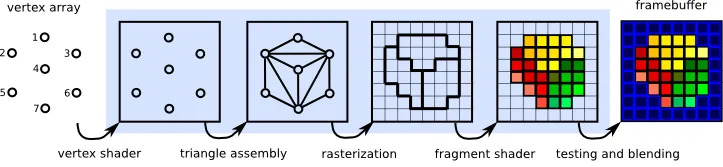
\includegraphics[width=0.9\textwidth]{pics/graphics-pipeline-raster.jpg}
	\caption{Vedere simplificată a pipeline-ului de rasterizare.\protect\footnotemark}
	\label{fig:rasterization-pipeline}
\end{figure}
\footnotetext{\copyright\url{https://bolt.graphics/}. Accesat 13.06.2026.}

\begin{figure}[ht]
	\centering
	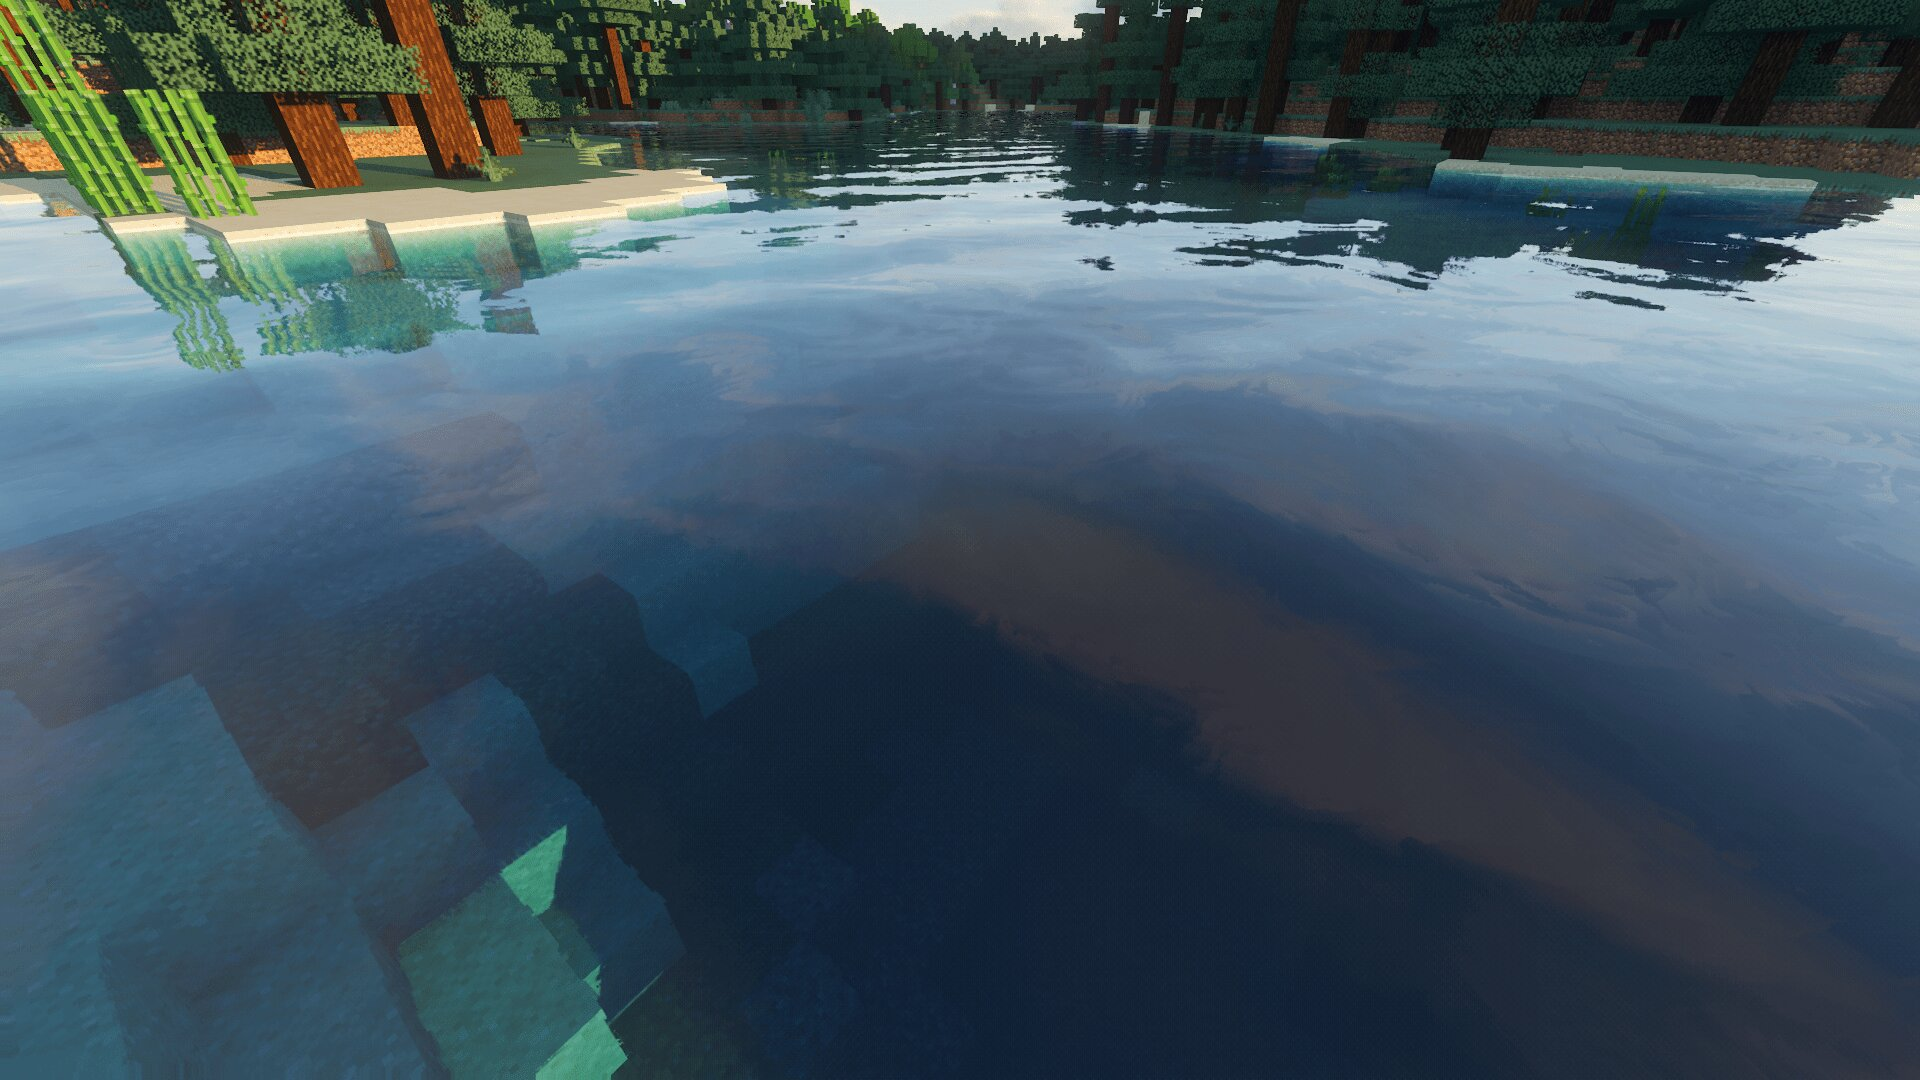
\includegraphics[width=0.9\textwidth]{pics/mc-ssr-bad.jpg}
	\caption{SSR nu capturează detaliile din scenă care nu sunt vizibile în spațiul ecranului (e.g., coamele copacilor de pe margine).\protect\footnotemark}
	\label{fig:rasterization-ssr}
\end{figure}
\footnotetext{\textcopyright Minecraft Continuum Shaders: \url{https://continuum.graphics/continuum-shaders/}. Accesat 13.06.2026.}

\section{Ray Tracing}

Spre deosebire de rasterizare, Ray Tracing rezolvă problemele vizibilității și iluminării prin simularea traiectoriilor razelor de lumină (de obicei în sens invers).

\textbf{Ray Casting} (Appel, 1968~\cite{Appel}) este varianta nerecursivă: raze primare determină vizibilitatea, raze secundare calculează umbrele.
Este un algoritm de vizibilitate fără componentă de iluminare.

\textbf{Ray Tracing recursiv} (Whitted, 1979~\cite{Whitted}, vezi Figura~\ref{fig:whitted-raytracing}) adaugă recursivitate: la fiecare intersecție se generează raze de reflexie, refracție și umbrire.
Reflexiile și refracțiile geometrice perfecte devin naturale, însă iluminarea difuză nu este modelată fizic.
Pentru aceasta, se poate utiliza un model Lambertian~\cite{Lambert}.

\begin{figure}[ht]
	\centering
	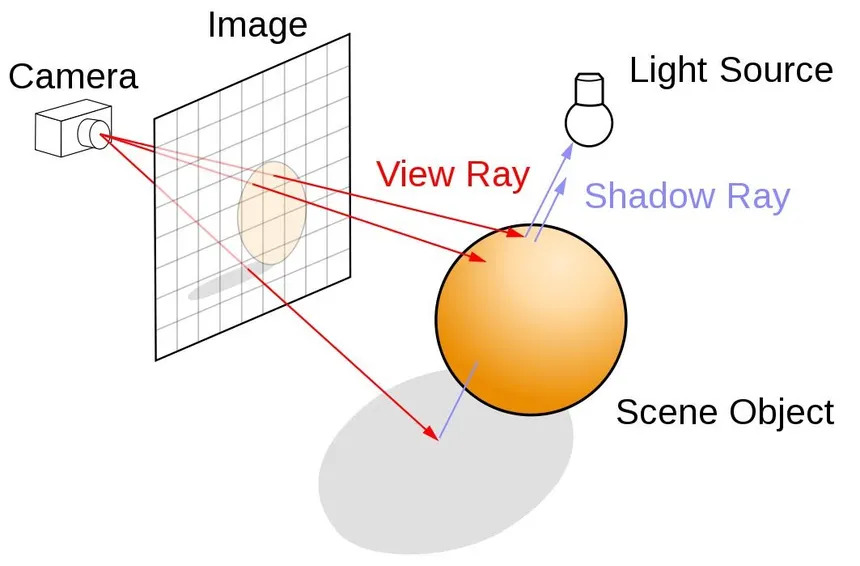
\includegraphics[width=0.7\textwidth]{pics/ray-tracing.jpg}
	\caption{Ray Tracing recursiv.\protect\footnotemark}
	\label{fig:whitted-raytracing}
\end{figure}
\footnotetext{\copyright\url{https://developer.nvidia.com/discover/ray-tracing}. Accesat 13.06.2026.}

\textbf{Ray Marching / Sphere Tracing} (Hart, 1996~\cite{hart1996sphere}, vezi Figura~\ref{fig:sphere-tracing}) este o variantă care nu calculează intersecții analitice, ci mărșăluiește de-a lungul razei folosind câmpuri de distanță cu semn (SDF).
La fiecare pas, algoritmul avansează cu distanța până la cea mai apropiată suprafață.
Se pot modela reflexii și refracții geometrice perfecte, la fel ca în Ray Tracing recursiv.
Este deosebit de util pentru suprafețe implicite și proceduale, sau pentru vizualizarea datelor volumetrice.

\begin{figure}[ht]
	\centering
	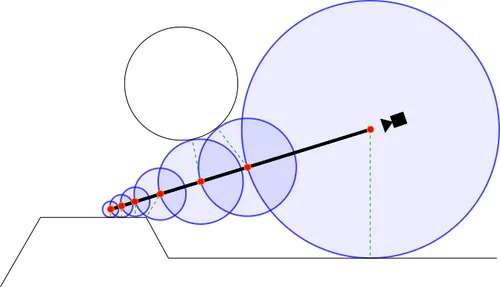
\includegraphics[width=0.7\textwidth]{pics/ray-marching.jpg}
	\caption{Iterațiile algoritmului Ray Marching.\protect\footnotemark}
	\label{fig:sphere-tracing}
\end{figure}
\footnotetext{\copyright\url{https://adrianb.io/2016/10/01/raymarching.html}. Accesat 13.06.2026.}

\section{Metode Monte Carlo}

Algoritmii de mai sus nu rezolvă complet ecuația de iluminare globală~(\ref{eq:light_transport}).
De aceea, au nevoie de metode aproximative de iluminare, precum Phong~\cite{Phong}, care nu sunt fizic corecte și nu pot reprezenta materiale complexe.
Metodele Monte Carlo eșantionează spațiul de soluții și aproximează integrala prin media ponderată a contribuțiilor eșantionate.
Dacă eșantionarea este realizată aleator, convergența este garantată, dar lentă ($\sim 1/\sqrt{N}$).

În practică, se utilizează două tehnici esențiale de accelerare a convergenței și de reducere a varianței estimatorului Monte Carlo:
\begin{itemize}
    \item \textbf{Eșantionare bazată pe importanță}: se eșantionează din distribuția $q(x)$ care aproximează $f(x)p(x)$, reducând varianța estimatorului (vezi~\cite{DieXaR2024}).
    \item \textbf{Eșantionare stratificată (jittering)}: domeniul se partiționează în straturi, iar câte un eșantion este ales din fiecare strat, evitând clusteringul aleator.
\end{itemize}

\subsection{Ecuația transportului luminii}

Introdusă de Kajiya~\cite{Kajiya} și Immel et al.~\cite{Immel} în 1986, ecuația
de randare este fundamentul teoretic al algoritmilor de iluminare globală:
\begin{equation}
    \label{eq:light_transport}
    \begin{aligned}
        L_o(\mathbf{x}, \omega_o) &= L_e(\mathbf{x}, \omega_o) + L_r(\mathbf{x}, \omega_o), \\
        L_r(\mathbf{x}, \omega_o) &= \int_{\Omega_+} f_r(\mathbf{x}, \omega_i, \omega_o)\,
            L_i(\mathbf{x}, \omega_i)\,(\omega_i \cdot \mathbf{n})\,\diff\omega_i.
    \end{aligned}
\end{equation}

Semnificația termenilor, cu referire la Figurile~\ref{fig:light_transport2} și~\ref{fig:light_transport}, este:
\begin{itemize}
    \item $\mathbf{x}$ -- punctul de incidență pe suprafață
    \item $\omega_o$ -- direcția de observare
    \item $\omega_i$ -- opusul direcției de incidență
    \item $\mathbf{n}$ -- normala la suprafață în $\mathbf{x}$
    \item $L_o$ -- radianța totală observată ($L_o = L_e + L_r$)
    \item $L_e$ -- radianța emisă de suprafață pe direcția $\omega_o$
    \item $L_r$ -- radianța reflectată/împrăștiată pe $\omega_o$, obținută prin
    integrarea contribuțiilor din toate direcțiile incidente $\omega_i \in \Omega_+$
    (emisfera superioară față de $\mathbf{n}$)
    \item $f_r(\mathbf{x}, \omega_i, \omega_o)$ -- BRDF-ul materialului: câtă lumină
    incidentă din $\omega_i$ este reflectată pe $\omega_o$
    \item $(\omega_i \cdot \mathbf{n})$ -- factorul de cosinus (legea Lambert):
    o suprafață absoarbe mai puțină lumină la unghiuri de incidență mari
\end{itemize}

\begin{figure}[ht]
	\centering
	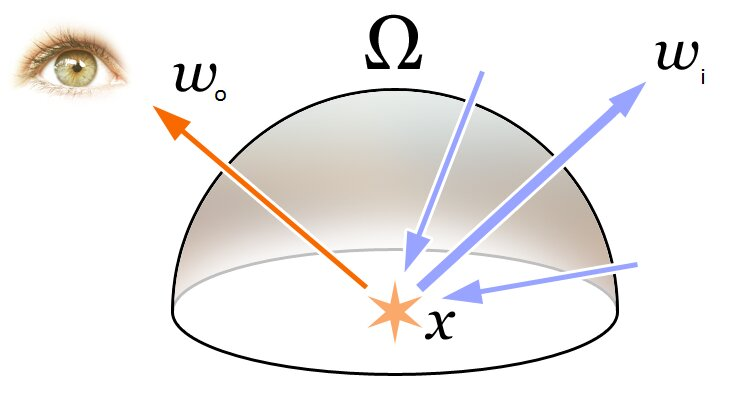
\includegraphics[width=0.7\textwidth]{pics/rendering_eq2.jpg}
	\caption{Ilustrație a componentelor din ecuația de randare.\protect\footnotemark}
	\label{fig:light_transport2}
\end{figure}
\footnotetext{\label{fn:wiki}\copyright\url{https://en.wikipedia.org/}. Accesat 20.06.2024.}

\begin{figure}[ht]
	\centering
	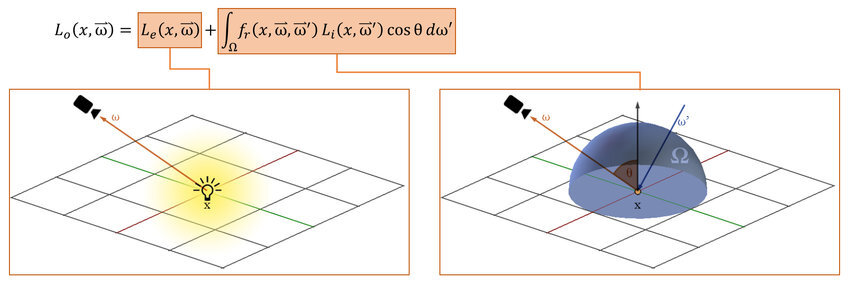
\includegraphics[width=0.9\textwidth]{pics/rendering_eq.jpg}
	\caption{Formă alternativă a ecuației transportului luminii. Se pot vedea componentele de emisie și împrăștiere.\protect\footnotemark}
	\label{fig:light_transport}
\end{figure}
\footnotetext{\copyright\url{https://www.researchgate.net/}. Accesat 13.06.2026.}

Ecuația poate fi augmentată cu un termen de transmisie (BTDF), integrând contribuțiile din emisfera inferioară $\Omega_-$ față de $\mathbf{n}$.
Combinând BRDF cu BTDF se obține BSDF (Bidirectional Scattering Distribution Function).

\subsection{Path Tracing}\label{sec:path_tracing}

Algoritmul Path Tracing rezolvă ecuația~(\ref{eq:light_transport}) numeric prin eșantionare Monte Carlo (vezi Algoritmul~\ref{alg:path_tracing}).
Funcționează pe același principiu ca Ray Tracing recursiv, însă razele de la fiecare intersecție sunt generate eșantionând informat următoarea direcție, în loc de a genera doar raze de reflexie și refracție geometrice perfecte.
Strategia de eșantionare a direcției de ieșire are un impact major: eșantionarea bazată pe importanță adaptată BSDF-ului converge mult mai rapid decât eșantionarea uniformă sau ponderată de cosinus.

\textbf{Next Event Estimation (NEE)} îmbunătățește convergența eșantionând explicit sursele de lumină la fiecare pas, combinând iluminarea directă (eșantionare lumini) cu cea indirectă (eșantionare BSDF) prin importanță multiplă (MIS)~\cite{Veach,VeachPower}.

\textbf{Ruleta rusească} termină recursivitatea prematur, în mod probabilistic, eliminând căile cu contribuție neglijabilă și redistribuind ponderea către căile rămase, pentru a menține conservarea energiei.

\section{Modele de materiale PBR}\label{sec:pbr}

Un BRDF corect fizic trebuie să satisfacă 3 restricții:
\begin{itemize}
	\item Pozitivitate: $f_r(\mathbf{x}, \omega_i, \omega_o) \geq 0$ pentru orice $\mathbf{x}$, $\omega_i$, $\omega_o$.
	\item Conservarea energiei: $\int_{\Omega_+} f_r(\mathbf{x}, \omega_i, \omega_o)\,(\omega_i \cdot \mathbf{n})\,\diff\omega_i \leq 1$ pentru orice $\mathbf{x}$ și $\omega_o$.
	\item Reciprocitate Helmholtz: $f_r(\mathbf{x}, \omega_i, \omega_o) = f_r(\mathbf{x}, \omega_o, \omega_i)$ pentru orice $\mathbf{x}$, $\omega_i$, $\omega_o$.
\end{itemize}

Cel mai popular model fizic este modelul \textbf{microfațetelor (Torrance-Sparrow)}~\cite{TorranceOld,CookTorrance}.
Suprafețele sunt modelate ca ansambluri de microfațete speculare orientate aleator.
BRDF-ul are forma:
\begin{equation}
    f_{TS} = \frac{D(\omega_h)\,G_2(\omega_i,\omega_o)\,F(\omega_o)}
             {4\,(\omega_i\cdot\mathbf{n})\,(\omega_o\cdot\mathbf{n})},
\end{equation}
unde $D$ este distribuția normalelor microfațetelor (NDF), $G_2$ modelează mascarea și umbrirea (Smith~\cite{SmithG1,WalterSmithG2}), iar $F$ este termenul Fresnel (aproximarea Schlick~\cite{Schlick}).

Modelul implementat în proiectul de diplomă și extins în această lucrare este \textbf{Disney Principled BSDF}~\cite{Disney,DisneyBSDF}.
Acest model a fost dezvoltat de Burley pentru producția Disney și a fost adoptat cu mici modificări în industrie (de exemplu, \textit{Principled BSDF} în Blender) datorită echilibrului său între realism și control artistic.
Combină 4 lobi -- difuz, specular, clearcoat și transmisie speculară, cu parametri normalizați și intuitivi pentru artiști (de aceea se și numește \textit{principiat}).
O ilustrație a parametrilor modelului se găsește în Figura~\ref{fig:disney_params}.

\section{Denoising și Upscaling}

Path Tracing este un algoritm care are nevoie de multe eșantioane per pixel pentru a scăpa de zgomot și a converge către o imagine stabilă.
Totodată, bugetul de calcul pentru Path Tracing în timp real ne limitează, în practică, la doar \textit{un singur eșantion per pixel} (1 spp).
Astfel, pentru a putea prezenta imagini cel puțin acceptabile vizual, este nevoie de tehnici de denoising și upscaling.
Denoising-ul elimină zgomotul Monte Carlo prin filtre spațio-temporale sau bazate pe inteligență artificială, în timp ce upscaling-ul creează imagini de rezoluție mai mare dintr-o imagine de rezoluție mai mică, păstrând detaliile vizuale.
Și acesta din urmă se poate folosi de filtre spațio-temporale sau metode bazate pe inteligență artificială.

\subsection{Metode Clasice de Denoising}

\textbf{Bilateral Filtering}~\cite{tomasi1998bilateral} este o tehnică care prezervă muchiile prin ponderarea pixelilor nu doar pe baza distanței spațiale, ci și pe baza similarității valorilor (e.g., culoare, adâncime).
În formularea originală, filtrul bilateral este definit ca:

\begin{equation}
	I_{\text{out}}(p) = \frac{1}{W_p} \sum_{q \in \Omega} I_{\text{in}}(q)\,c(\|q-p\|)\,s(\|I_{\text{in}}(q)-I_{\text{in}}(p)\|),
\end{equation}
cu factor de normalizare
\begin{equation}
	W_p = \sum_{q \in \Omega} c(\|q-p\|)\,s(\|I_{\text{in}}(q)-I_{\text{in}}(p)\|),
\end{equation}
iar pentru nuclee Gaussiene:
\begin{equation}
	c(d)=\exp\left(-\frac{d^2}{2\sigma_s^2}\right), \qquad
	s(r)=\exp\left(-\frac{r^2}{2\sigma_r^2}\right).
\end{equation}
Pe scurt, parametrii au următorul rol:
\begin{itemize}
	\item $\Omega$ -- vecinătatea (fereastra locală) în jurul pixelului $p$
	\item $\sigma_s$ -- lățimea componentei spațiale; valori mai mari înseamnă netezire pe o arie mai mare
	\item $\sigma_r$ -- lățimea componentei de range; valori mici păstrează mai bine muchiile
\end{itemize}

\textbf{Non-Local Means (NLM)}~\cite{BcmNlm} este o extensie a filtrului bilateral, care compară zone mari de pixeli în loc de valori singulare, fiind mai eficace la zgomotul Monte Carlo de frecvență mare.
Comparația pe bază de zone permite o ponderare mai informată și reduce artefactele de blur.

\textbf{Edge-Aware Filtering} combină informații de geometrie (normale, adâncime, UV) cu informații de luminanță pentru a reduce zgomotul selectiv și a păstra caracteristicile importante ale scenei.
NVIDIA \textbf{Real-time Denoisers (NRD)}\footref{nrd} implementează mai multe strategii de edge-aware filtering, printre care:
\begin{itemize}
	\item REBLUR -- denoiser bazat pe blur recurent.
	\item RELAX -- denoiser bazat pe \`A-Trous~\cite{dammertz2010edge}.
	\item SIGMA -- denoiser pentru umbre, per-lumină.
\end{itemize}

Aceste metode sunt rapide și deterministe (nu sunt bazate pe inteligență artificială), însă convergența în scenele complexe rămâne limitată și pot introduce artefacte pe tranziții complexe.

\subsection{SVGF și A-SVGF}

O metodă de referință pentru denoising în Path Tracing este \textbf{SVGF} (\textit{Spatiotemporal Variance-Guided Filtering})~\cite{schied2017spatiotemporal}.
Ideea principală este combinarea unui filtru temporal cu un filtru spațial ghidat de varianță, astfel încât zonele stabile să fie netezite agresiv, iar zonele instabile (muchiile, dezocluziile, reflexiile) să fie tratate conservativ, pentru a păstra detaliile.

Filtrul temporal acumulează informații din cadrele anterioare, reproiectând pixelii în funcție de mișcarea camerei și a obiectelor.
Acest lucru este făcut folosind \textit{motion vectors}, cu mențiunea că reproiectarea poate introduce ghosting dacă mișcarea este rapidă sau dacă există dezocluzii.

Filtrul spațial este un filtru clasic de tip wavelet \`A-Trous~\cite{dammertz2010edge}, care are rolul de a reduce zgomotul unei imagini deja generate.
Acest filtru este edge-aware, prin prisma faptului că este ghidat de varianța pixelilor (calculată în cadrul filtrului temporal) -- astfel, pixelii cu varianță mare (de obicei în jurul muchiilor) sunt neteziți mai puțin, pentru a păstra detaliile.

În practică, SVGF produce o reducere semnificativă a zgomotului la 1 spp, cu cost rezonabil pentru aplicații în timp real, motiv pentru care a devenit fundamentul pentru multe implementări ulterioare.

\textbf{A-SVGF} (\textit{Adaptive Spatiotemporal Variance-Guided Filtering})~\cite{schied2018gradient} extinde SVGF prin mecanisme adaptive care ajustează local acumularea și filtrarea în funcție de stabilitatea semnalului.
Îmbunătățirea majoră pe care o aduce acest algoritm față de SVGF este reducerea ghosting-ului și a artefactelor în zonele cu mișcare rapidă sau dezocluzii.
Comparații între SVGF și A-SVGF se pot observa în Figurile~\ref{fig:asvgf} și~\ref{fig:asvgf2}.

\begin{figure}[ht]
	\centering
	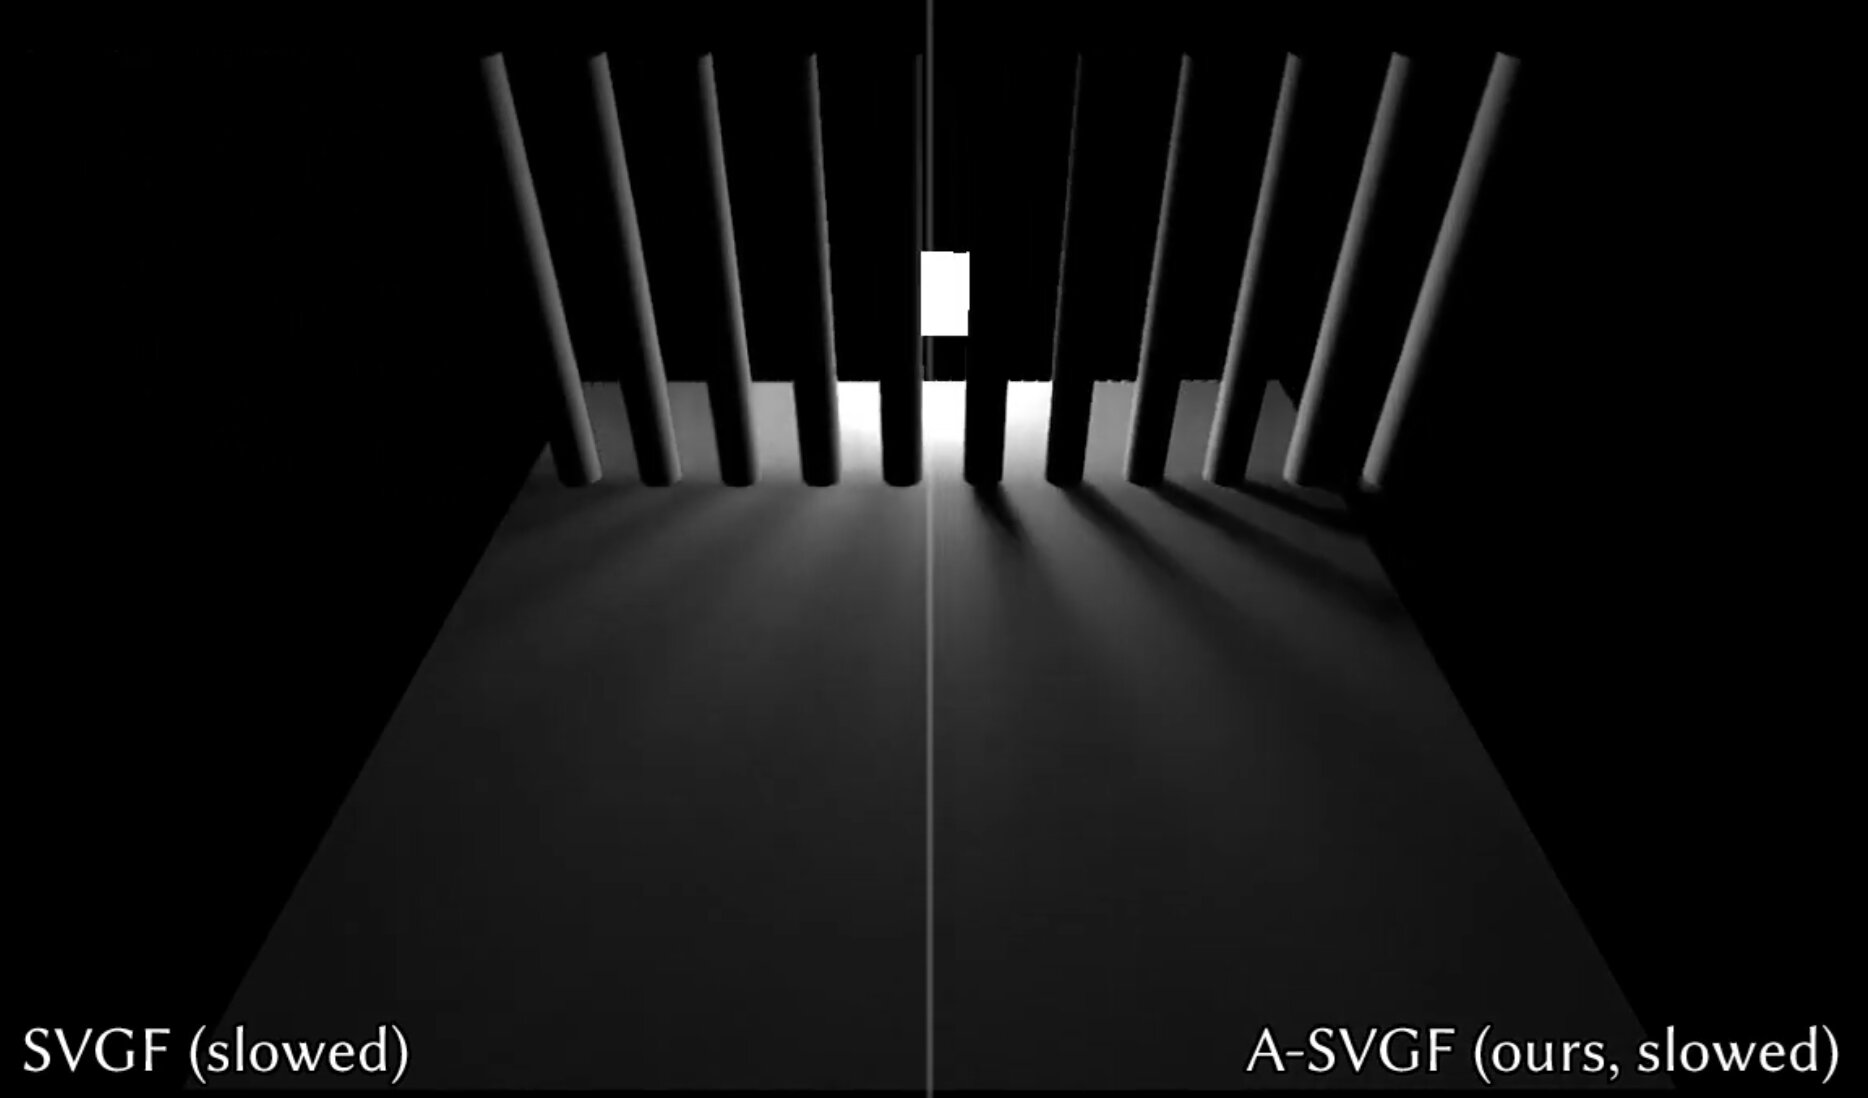
\includegraphics[width=0.9\textwidth]{pics/asvgf.jpg}
	\caption{Comparație SVGF vs A-SVGF. Se poate observa ghosting masiv în varianta non-adaptivă.\protect\footref{footnote:asvgf}}
	\label{fig:asvgf}
\end{figure}

\begin{figure}[htb]
	\centering
	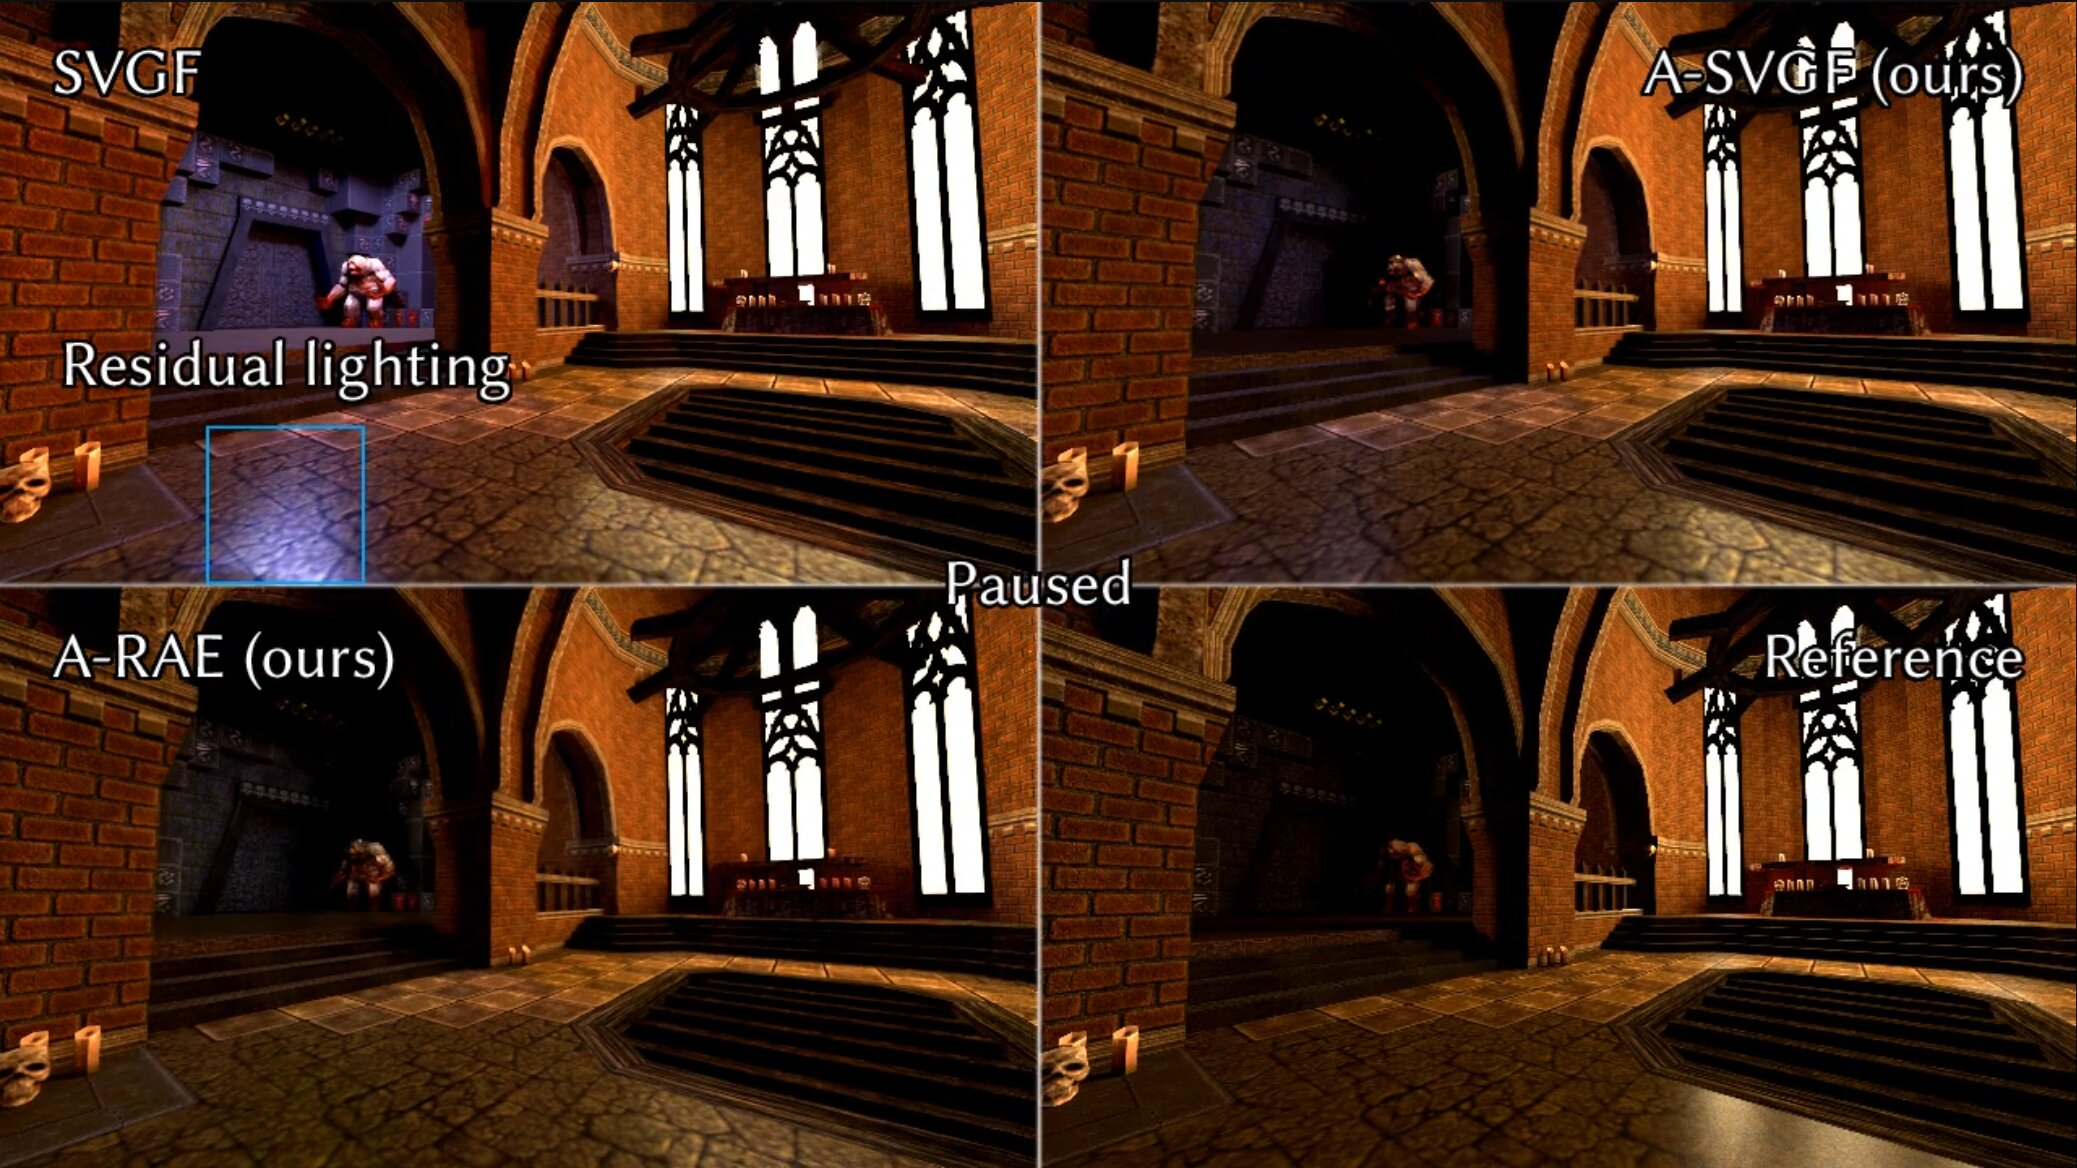
\includegraphics[width=0.9\textwidth]{pics/asvgf2.jpg}
	\caption{Comparație SVGF vs A-SVGF. Se poate observa cum varianta non-adaptivă suferă în medii cu iluminare care se schimbă brusc.\protect\footnotemark}
	\label{fig:asvgf2}
\end{figure}
\footnotetext{\label{footnote:asvgf}\textcopyright Christoph Schied: \url{https://www.youtube.com/watch?v=Fv-jStEsCpE}. Accesat 14.06.2026.}

\subsection{Denoising cu Deep Learning}

Până acum am vorbit despre metode de denoising bazate pe filtre spațiale și temporale, care sunt rapide și deterministe, dar au limitări în scenele complexe.
Rețelele neurale pot învăța reprezentări implicite ale zgomotului și pot executa denoise-ul cu o precizie care depășește metodele clasice.
Acestea sunt antrenate pe seturi mari de imagini realizate cu Path Tracing cu zgomot mare și imagini de referință fără zgomot, învățând să mapeze intrările zgomotoase la ieșiri curate.

Pe partea de open-source, avem câteva exemple notabile care se pretează la denoising în timp real:
\begin{itemize}
	\item \textbf{OptiX AI Denoiser}~\cite{optix2017} -- denoiser oferit de NVIDIA ca parte a OptiX SDK.
	\item \textbf{Intel Open Image Denoise}~\cite{OpenImageDenoise} -- bibliotecă open-source cu modele pentru CPU și GPU.
\end{itemize}

Pe plan comercial, NVIDIA DLSS Ray Reconstruction\footnote{\url{https://www.nvidia.com/en-us/geforce/news/dlss-4-5-ray-reconstruction-1000-rtx-games-apps-out-now/}. Accesat 14.06.2026.} și AMD FSR Ray Regeneration\footref{footnote:fsr_ray_regeneration} sunt exemple de denoising bazat pe deep learning.
Intel XeSS va oferi în viitorul apropiat o soluție similară pentru GPU-urile Arc\footnote{\url{https://wccftech.com/intel-enabling-high-fidelity-visuals-faster-performance-on-built-in-gpus-demos-ray-reconstruction-path-tracing-arc-b580/}. Accesat 14.06.2026.}.

\subsection{Upscaling}

Upscaling-ul reprezintă o tehnică importantă de optimizare, ce oferă posibilitatea de a randa la o rezoluție internă mai mică și a genera o imagine de rezoluție mai mare printr-un proces de super-rezoluție.
În contextul nostru, se adaugă și cerința de a reconstitui detaliile vizuale care se pierd prin randarea la o rezoluție mai mică.

Upscaling-ul tradițional folosește interpolare (biliniară, bicubică) sau filtre mai sofisticate (Lanczos~\cite{duchon1979lanczos}), dar produce rezultate \textit{soft} și nu poate recupera detaliile pierdute.
Există și metode analitice, bazate pe algoritmi spațiali (AMD FSR 1\footnote{\url{https://gpuopen.com/manuals/fidelityfx_sdk/techniques/super-resolution-spatial/}. Accesat 14.06.2026.}) sau chiar spațio-temporali (AMD FSR 2 și 3\footnote{\url{https://gpuopen.com/manuals/fidelityfx_sdk/techniques/super-resolution-upscaler/}. Accesat 14.06.2026.}), care reușesc să păstreze detaliile vizuale mai bine, dar tot nu pot atinge calitatea unui model bazat pe inteligență artificială.

\textbf{Upscaling-ul neural} marchează o tranziție fundamentală.
Soluțiile oferite de vendori folosesc modele de deep learning și accelerare hardware pentru inferență în timp real, de multe ori producând rezultate mai plăcute vizual decât folosirea unor algoritmi de anti-aliasing nativi precum TAA.
Cele mai populare soluții sunt:
\begin{itemize}
	\item \textbf{DLSS (Deep Learning Super Sampling)} -- tehnologia NVIDIA, de obicei fiind apreciată drept cea mai bună implementare. Rulează exclusiv pe hardware NVIDIA RTX.
		\begin{itemize}
			\item \textbf{DLSS 3.x} -- folosește rețele neurale convoluționale (CNN), ce lucrează local folosind kernele.
			\item \textbf{DLSS 4.0/4.5} -- introduce o arhitectură de tip Transformer, ce poate folosi informații globale din întreaga imagine.
		\end{itemize}
	\item \textbf{FSR (FidelityFX Super Resolution) 4} -- soluția AMD, bazată pe un model hibrid CNN--Transformer. Rulează exclusiv pe hardware AMD RDNA 4 și DirectX 12, cu suport oficial pentru RDNA 3 și RDNA 2 venind în viitorul apropiat.
	\item \textbf{XeSS (Xe Super Sampling)} -- soluția Intel, bazată pe un model proprietar. Rulează cu accelerare hardware pe GPU-urile Arc (modul XMX), sau cu suport software (modul DP4a) pentru alte platforme.
\end{itemize}


\chapter{\label{sec:solutie}Soluție Propusă}

Acest proiect de diplomă propune un motor grafic -- \texttt{Vlkrt}\footnote{\url{https://github.com/nurof3n/vlkrt}. Accesat 14.06.2026.} -- care implementează un pipeline de Ray Tracing în timp real, cu suport pentru iluminare globală prin Path Tracing.
Tehnologia care stă la baza acestui motor este Vulkan 1.4, iar implementarea este realizată în C++, folosind standardul modern C++20.

În primul rând, \texttt{Vlkrt} reprezintă, fundamental, o portare a motorului de Ray Tracing \texttt{DieXaR}\footnote{\url{https://github.com/nurof3n/diexar}. Accesat 14.06.2026.}~\cite{DieXaR2024} către o arhitectură modernă, modulară și extensibilă, bazată pe API-ul portabil, low-level -- Vulkan.
Algoritmul de Path Tracing de la bază este același, împreună cu implementările de BSDF ale sistemului de materiale principiat de la Disney~\cite{Disney,DisneyBSDF}.
Nu vom mai trece prin detalii legate de aceste două componente, pentru că au fost acoperite în detaliu în lucrarea de diplomă.

În procesul de portare am tradus shader-ele HLSL în Slang, un limbaj modern întreținut de Khronos Group, compatibil cu ideologia de portabilitate -- acesta permite compilare multiplatformă și suport pentru multiple backend-uri grafice (Vulkan, DirectX, Metal, OpenGL, CUDA, WebGPU).
Așadar, am păstrat algoritmul de Path Tracing și varianta sa cu acumulare temporală, precum și tehnicile de accelerare a convergenței aferente -- eșantionarea bazată pe importanță (a BSDF-ului), Next Event Estimation, eșantionarea unei singure lumini în scenă și ruleta rusească.
De asemenea, \texttt{Vlkrt} poate randa atât mesh-uri tradiționale, cât și suprafețe analitice (e.g., sfere) și implicite (definite prin SDF-uri).
Aceste lucruri sunt demonstrate prin portarea celor 3 scene de test din \texttt{DieXaR}.

Scopul motorului grafic propus în această lucrare este de a extinde funcționalitățile motorului precedent și de a îmbunătăți experiența utilizatorului.
Așadar, \texttt{Vlkrt} adaugă funcționalități pe mai multe planuri, pe care le vom prezenta în secțiunea~\ref{sec:implementare}.
Într-o vedere de ansamblu, \texttt{Vlkrt} permite utilizatorului să descrie scene custom într-un format YAML, să definească logica obiectelor din scenă prin scripting în Lua, să interacționeze cu scena în timp real și să partajeze starea avatarului cu alți utilizatori printr-un sistem de rețea client-server.
În anexă se pot studia câteva capturi de ecran care demonstrează aceste funcționalități (vezi Figurile~\ref{fig:conectare_server},~\ref{fig:scene_editor} și~\ref{fig:vlkrt_ansamblu}).

\texttt{Vlkrt} aduce îmbunătățiri și pe partea grafică, integrând denoiser-ul NRD și upscaler-ul AMD FSR 3, menite să crească fidelitatea imaginii, menținând performanța în timp real.

\chapter{\label{sec:implementare}Detalii de implementare}

În acest capitol vom discuta despre arhitectura generală a motorului grafic \texttt{Vlkrt} și vom intra în detalii tehnice acolo unde este cazul.
Fiecare subcapitol va acoperi o componentă de interes.

\section{Framework extensibil}


La baza aplicației se află framework-ul Walnut\footnote{\url{https://github.com/nurof3n/walnut}. Accesat 14.06.2026.}, care oferă un strat subțire de abstractizare peste gestionarea resurselor de bază ale Vulkan și rulează aplicația \texttt{Vlkrt}.
Acesta se ocupă de:
\begin{itemize}
    \item \textbf{Gestionarea ferestrelor și a contextului:} Walnut utilizează \texttt{GLFW} sub capotă pentru crearea ferestrelor și gestionarea contextului de execuție.
    \item \textbf{Gestiunea resurselor Vulkan:} Framework-ul abstractizează concepte precum \textit{Command Pool} și \textit{Swapchain}.
        Spre exemplu, clasa \texttt{Renderer} obține un \texttt{VkCommandBuffer} valid pentru fiecare frame prin \texttt{Walnut::Application::GetCommandBuffer()}.
        De asemenea, pentru a gestiona ștergerea resurselor utilizate de GPU în mod asincron (și a evita situații precum buffer-e distruse în timp ce sunt încă în uz într-un frame anterior), se folosește coada de eliberare a resurselor prin \texttt{SubmitResourceFree()}.
    \item \textbf{Sistem de layer-ing:} Arhitectura este bazată pe un sistem de \textit{Layers}, similar cu cel din motoarele grafice moderne.
        Orice funcționalitate nouă este implementată ca un \texttt{Layer} (e.g., \texttt{ClientLayer}, \texttt{ServerLayer}), care primește evenimente de \texttt{OnUpdate()}, \texttt{OnRender()} și \texttt{OnUIRender()}.
    \item \textbf{Networking:} Walnut oferă suport pentru comunicații de rețea reliable prin UDP, folosind biblioteca \texttt{GameNetworkingSockets}\footnote{\label{fn:gamesocket}\url{https://github.com/ValveSoftware/GameNetworkingSockets}. Accesat 14.06.2026.} de la Valve.
    \item \textbf{Imagini:} Clasa \texttt{Walnut::Image} încapsulează crearea \texttt{VkImage}, \texttt{VkImageView} și a descriptorilor necesari pentru a afișa rezultatul randării în \texttt{ImGui}\footnote{\url{https://github.com/ocornut/imgui}. Accesat 14.06.2026.}.
    \item \textbf{Integrare ImGui:} Framework-ul oferă o integrare \textit{out-of-the-box} cu \texttt{ImGui} pentru crearea rapidă de interfețe de utilizator reactive, optimizând procesul de dezvoltare.
        Buffer-ul de afișare folosit pentru ieșirea algoritmului de Path Tracing este de asemenea gestionat de către \texttt{ImGui}.
\end{itemize}

\section{Arhitectură client-server}

Proiectul a fost gândit de la început ca o aplicație client-server, cu scopul de a permite gameplay multiplayer.
Acesta nu a fost punctul de focus principal, așadar implementarea este doar demonstrativă.
Pentru a putea face posibilă această arhitectură, \texttt{Vlkrt} este compus din 3 module principale:

\subsection{Vlkrt-Client}

Clientul reprezintă componenta principală de interfațare cu utilizatorul și motorul de vizualizare.
Acesta conține:
\begin{itemize}
    \item \textbf{Motor de randare:} Utilizează Vulkan SDK pentru un control granular asupra pipeline-ului de randare.
        Acesta este configurat pentru a utiliza extensiile de Ray tracing hardware (\texttt{VK\_KHR\_ray\_tracing\_pipeline}).
    \item \textbf{Procesare de input:} Gestionează camera și interacțiunile de mouse/tastatură prin intermediul framework-ului \texttt{Walnut}.
        În spate, \texttt{Walnut} folosește de fapt API-ul \texttt{GLFW}.
    \item \textbf{Motor de scripting:} Include un motor de scripting bazat pe \texttt{Lua} (via \texttt{Sol2}\footnote{\url{https://github.com/ThePhD/sol2}. Accesat 14.06.2026.} și \texttt{LuaJIT}\footnote{\url{https://luajit.org/}. Accesat 14.06.2026.}), permițând definirea de logică custom pentru obiectele din scenă, fără recompilarea codului C++.
\end{itemize}

\subsection{Vlkrt-Server}

Serverul este o aplicație \textit{headless} responsabilă pentru sincronizarea stării jocului.
Acesta nu inițializează contextul Vulkan pentru randare, utilizând în schimb o variantă minimală a \texttt{Walnut} (\texttt{Walnut-Headless}).
Atribuții:
\begin{itemize}
    \item \textbf{State Management:} Menține o bază de date în memorie cu toți utilizatorii conectați.
    \item \textbf{Packet Handling:} Procesează cererile primite de la clienți și replică modificările către toți ceilalți participanți în timp real.
\end{itemize}

Comunicarea între clienți și server este gestionată de submodulul \texttt{Walnut-Networking}\footnote{\url{https://github.com/nurof3n/Walnut-Networking/}. Accesat 14.06.2026.}, care utilizează biblioteca \texttt{GameNetworkingSockets}\footref{fn:gamesocket} de la Valve pentru o comunicare bazată pe UDP, optimizată pentru latență redusă.
Caracteristici:
\begin{itemize}
    \item \textbf{Modelul de date:} Schimbul de informații se bazează pe pachete binare.
        Mesajele sunt serializate într-un format compact pentru a minimiza utilizarea lățimii de bandă.
    \item \textbf{Sincronizarea stării:} Clientul trimite periodic actualizări ale poziției și stării proprii, în timp ce serverul transmite aceste date către ceilalți clienți conectați pentru a reconstrui scena globală.
    \item \textbf{Gestiunea conexiunilor:} Serverul implementează logica de acceptare/respingere a conexiunilor și de gestionare a deconectărilor.
    \item \textbf{Chat}: Clienții conectați pot comunica printr-un chat comun.
    \item \textbf{Server tickrate:} Pentru eficiență, serverul limitează procesarea pachetelor la o frecvență de 50Hz. Aceasta se poate crește cu ușurință.
\end{itemize}

În listarea~\ref{lst:packet_example} se poate vedea un exemplu de trimitere a unui update de la client la server, folosind \texttt{Walnut::BufferStreamWriter} pentru a construi un pachet binar compact.

\begin{lstlisting}[caption={Exemplu de trimitere a unui update de la client la server.}, language=C++, label=lst:packet_example, frame=single]
// Exemplu: Trimitere update de la client la server
void ClientLayer::OnUpdate(float ts)
{
    // ...
    if (m_Client.GetConnectionStatus() == 
        Walnut::Client::ConnectionStatus::Connected)
    {
        Walnut::BufferStreamWriter stream(s_ScratchBuffer);
        
        // Scrie tip pachet si date player
        stream.WriteRaw(PacketType::ClientUpdate);
        stream.WriteRaw<glm::vec3>(m_PlayerPosition);
        stream.WriteRaw<glm::vec3>(m_PlayerVelocity);
        
        m_Client.SendBuffer(stream.GetBuffer());
    }
}
\end{lstlisting}

Modelul de sincronizare între clienți este unul primitiv.
Astfel, la pornirea aplicației, clientului îi este solicitat să introducă adresa serverului și portul pentru conexiune.
După stabilirea conexiunii, se randează scena Cornell Box, în care apare un cub ce poate fi controlat de jucător.
Ceilalți clienți conectați vor fi reprezentați ca alte cuburi și se va face sincronizarea transformărilor acestora în timp real.

\subsection{Vlkrt-Common}

Această bibliotecă statică conține simboluri partajate între binarele de client și server pentru a asigura consistența datelor.
Aici se definesc structurile pachetelor de rețea (\texttt{ServerPacket.h} și \texttt{UserInfo.h}). 

\section{Gestiune de resurse}

Un aspect critic al proiectului este încărcarea și organizarea eficientă a resurselor digitale (mesh-uri, scene, texturi).

\subsection{Mesh-uri}

Clasa \texttt{MeshLoader} utilizează biblioteca \texttt{tinyobjloader}\footnote{\url{https://github.com/tinyobjloader/tinyobjloader}. Accesat 14.06.2026.} pentru a încărca fișiere de tip \texttt{.obj}.
După încărcare, se calculează automat normalele (dacă lipsesc) și coordonatele de textură.

Se folosește un format custom pentru a reține informații precum buffer-ele de vertecși și indecși, sau matricea de model (vezi listarea~\ref{lst:mesh_structures}).
Se pot crea și obiecte în mod procedural, spre exemplu se pot folosi funcțiile \texttt{GenerateQuad} și \texttt{GenerateCube}.

\begin{lstlisting}[caption={Structuri pentru vertecși și mesh-uri.}, language=C++, label={lst:mesh_structures}, frame=single]
struct Vertex
{
	glm::vec3 Position{};
	glm::vec3 Normal{};
	glm::vec2 TexCoord{};
};
struct Mesh
{
	std::string Filename;
	std::string Name;
	std::vector<Vertex> Vertices;
	std::vector<uint32_t> Indices;
	glm::mat4 Transform = glm::mat4(1.0f);
	uint32_t MaterialIndex{ 0 };
};
\end{lstlisting}

\subsection{Materiale}

\texttt{Vlkrt} folosește modelul de materiale principiat de la Disney~\cite{Disney,DisneyBSDF}, care combină 4 lobi -- difuz, specular, clearcoat și transmisie speculară.
La aceste proprietăți se adaugă și un canal de textură albedo, care poate fi încărcat dintr-un fișier extern.
Structura care conține aceste proprietăți, precum și explicații pentru fiecare dintre ele, se găsește în Listarea~\ref{lst:material_structures}.
De asemenea, în Figura~\ref{fig:disney_params} se poate vedea o ilustrație a parametrilor modelului, iar în Figura~\ref{fig:materiale} se poate vedea o scenă cu materiale randomizate în cadrul \texttt{Vlkrt}.

\begin{figure}[ht]
	\centering
	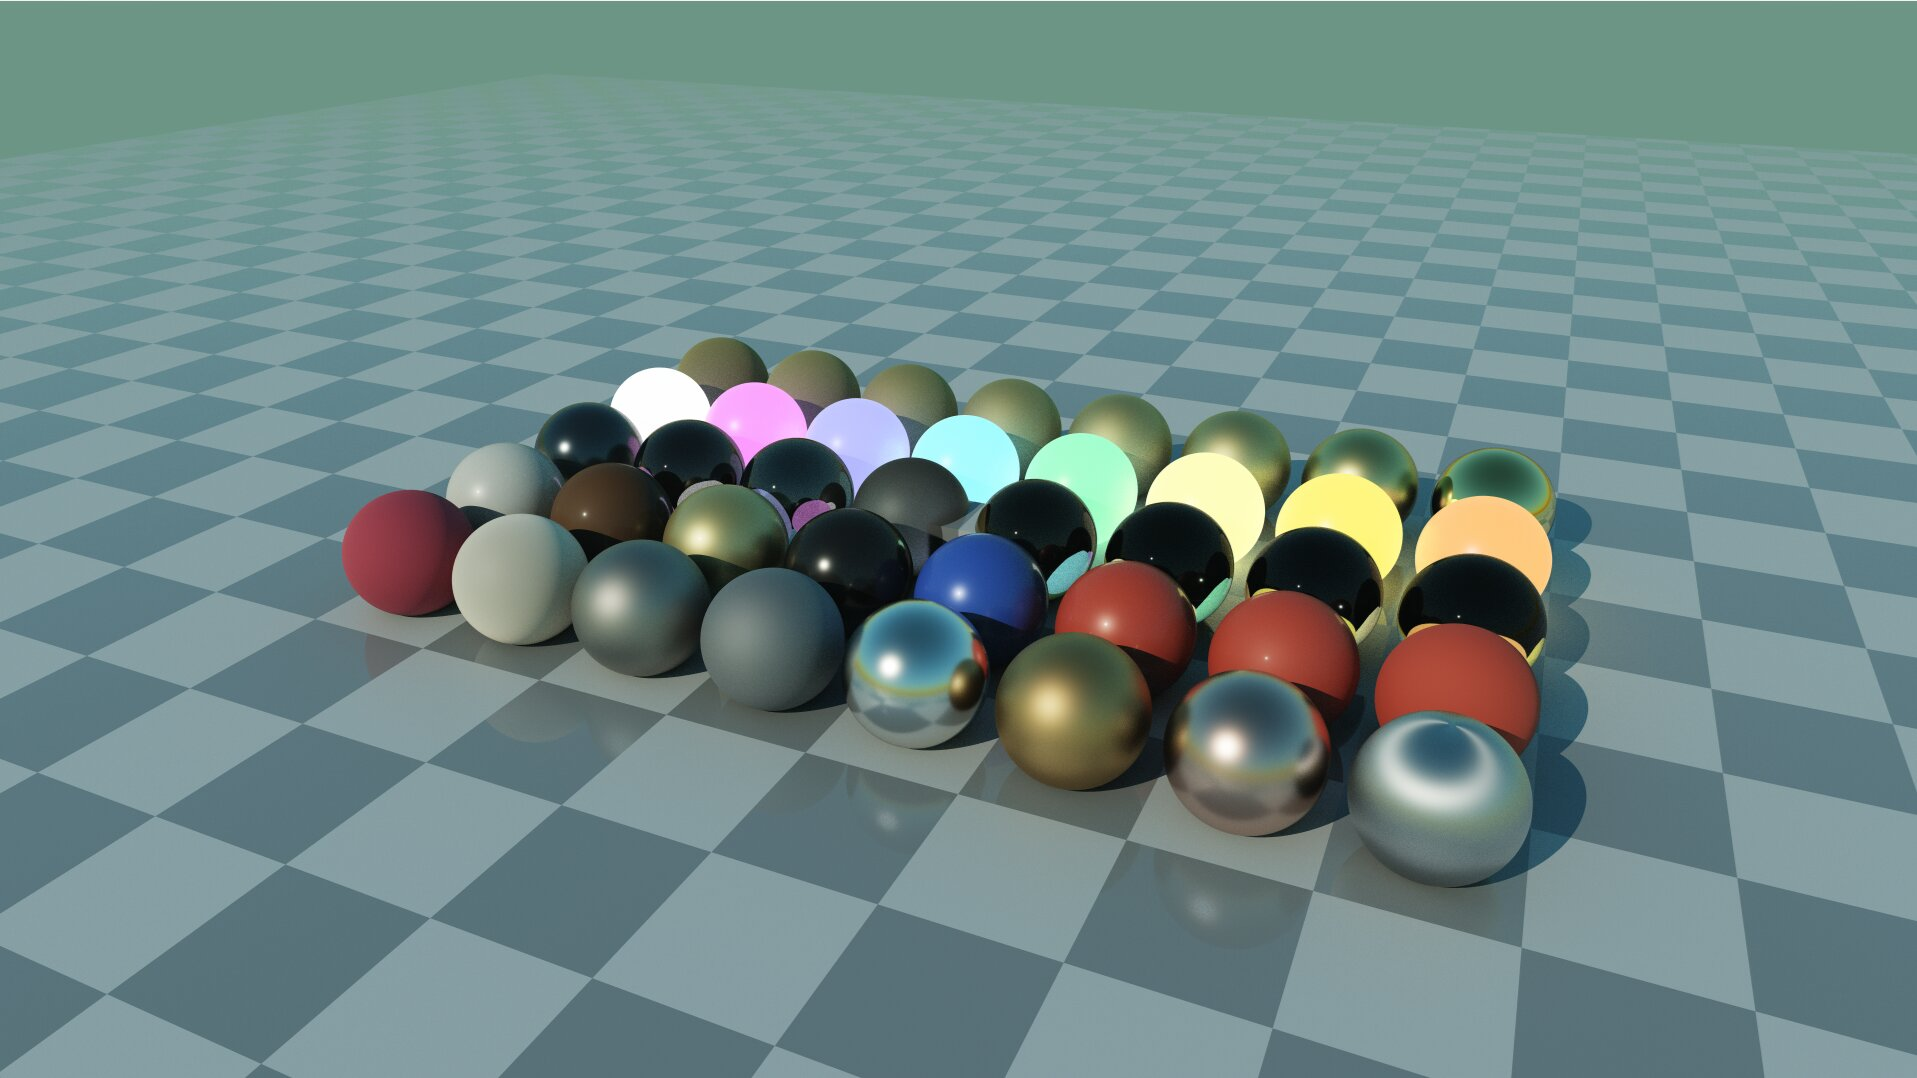
\includegraphics[width=0.9\textwidth]{pics/materiale.jpg}
	\caption{Scenă de test pentru materiale randomizate.}
	\label{fig:materiale}
\end{figure}

\texttt{Vlkrt} suportă încărcarea de texturi prin intermediul bibliotecii \texttt{stb\_image}\footnote{\url{https://github.com/nothings/stb}. Accesat 14.06.2026.}.
Resursele de tip imagine sunt gestionate prin clasa \texttt{Walnut::Image}.
Sunt suportate diferite formate, precum JPEG și PNG (teoretic și HDR, dar nu este suport în shader-e).
De asemenea, utilizatorul poate schimba texturile materialelor din GUI și aplica factori diferiți de tiling.

\subsection{Shader-e}

Shader-ele sunt scrise în Slang și compilate în format intermediar SPIR-V folosind \texttt{slangc}.
Pasul de compilare trebuie gestionat separat de compilarea aplicației, care încarcă direct codul SPIR-V la runtime.
Proiectul include script-uri de compilare pentru Windows și Linux ale shader-elor.
Pentru mai multe detalii vezi Secțiunea~\ref{sec:rendering}.

\subsection{Script-uri}

Script-urile Lua sunt încărcate on-demand la primul update al fiecărui obiect scriptat.
Mai multe detalii în Secțiunea~\ref{sec:scripting}.

\subsection{Scene}

\subsubsection{Sistem ierarhic}

\texttt{Vlkrt} utilizează un sistem ierarhic de entități, în care fiecare obiect din lume are o transformare relativă față de părintele său.
Fiecare entitate deține o structură \texttt{Transform} care stochează separat poziția (\texttt{vec3}), rotația (\texttt{quat} - cuaternioni pentru evitarea fenomenului \textit{Gimbal Lock}) și scalarea (\texttt{vec3}).
Matricea de transformare globală (\texttt{WorldTransform}) este recalculată recursiv atunci când este necesar: $M_{world} = M_{parent\_world} \times M_{local}$.
Sistemul suportă multiple tipuri de entități: \texttt{Mesh} (geometrie), \texttt{Light} (surse de lumină), și \texttt{Empty} (folosite pentru gruparea logică a obiectelor).

\subsubsection{Serializare}

Scenele sunt salvate și încărcate utilizând formatul YAML.
\texttt{yaml-cpp}\footnote{\url{https://github.com/jbeder/yaml-cpp}. Accesat 14.06.2026.} este biblioteca utilizată pentru parsarea și generarea fișierelor YAML.
Acestea reflectă ierarhia entităților din scenă, fiecare entitate având un câmp \texttt{children} care conține sub-entitățile sale, facilitând organizarea logică a scenei.
Toate proprietățile entităților (poziție, rotație, scalare, materiale etc.) sunt serializate, permițând salvarea progresului într-un fișier ușor de citit de către om (vezi Listarea~\ref{lst:scene_example}).
Modificările se pot salva și în timp real, din cadrul GUI-ului de editare a scenei.
Sistemul permite reîncărcarea la runtime a scenelor fără repornirea aplicației, facilitând iterarea rapidă asupra design-ului.

\subsubsection{Editor de scene}

Clientul include un editor vizual (vezi Figura~\ref{fig:scene_editor}) cu următoarele funcționalități:
\begin{itemize}
    \item \textbf{Arborele de entități:} Afișează o reprezentare ierarhică a tuturor obiectelor din scenă. Utilizatorul poate:
        \begin{itemize}
            \item Selecta entități în arbore.
            \item Extinde/restrânge noduri pentru a vizualiza relațiile părinte-copil.
            \item Modifica, salva și încărca scene.
        \end{itemize}
    \item \textbf{Inspector de proprietăți:} Afișează detaliile entității selectate:
        \begin{itemize}
            \item \textbf{Transform Controls:} Câmpuri pentru poziție (X, Y, Z), pentru rotație Euler (pitch, yaw, roll) și pentru scalare. Schimbările sunt aplicate imediat.
            \item \textbf{Material Properties:} Selectare de material dintr-o listă, ajustare a parametrilor BSDF-ului. Texturile pot fi selectate dintr-o listă a fișierelor disponibile.
            \item \textbf{Light Properties:} Pentru entități de tip lumină, oferă control pentru culoare, direcție (la lumini direcționale), intensitate, și dimensiune (la lumini de tip suprafață).
            \item \textbf{Script Path:} Permite atribuirea unui script Lua unei entități.
        \end{itemize}
    \item \textbf{Chat:} Acceptă input de la utilizator și afișează toate mesajele stocate pe server.
    \item \textbf{Statistics Panel:} Afișează:
        \begin{itemize}
            \item ID-ul jucătorului.
            \item Coordonatele și direcția camerei.
            \item Timing-uri și metrici (vezi Secțiunea~\ref{sec:evaluare}).
        \end{itemize}
\end{itemize}

\begin{figure}[H]
    \centering
    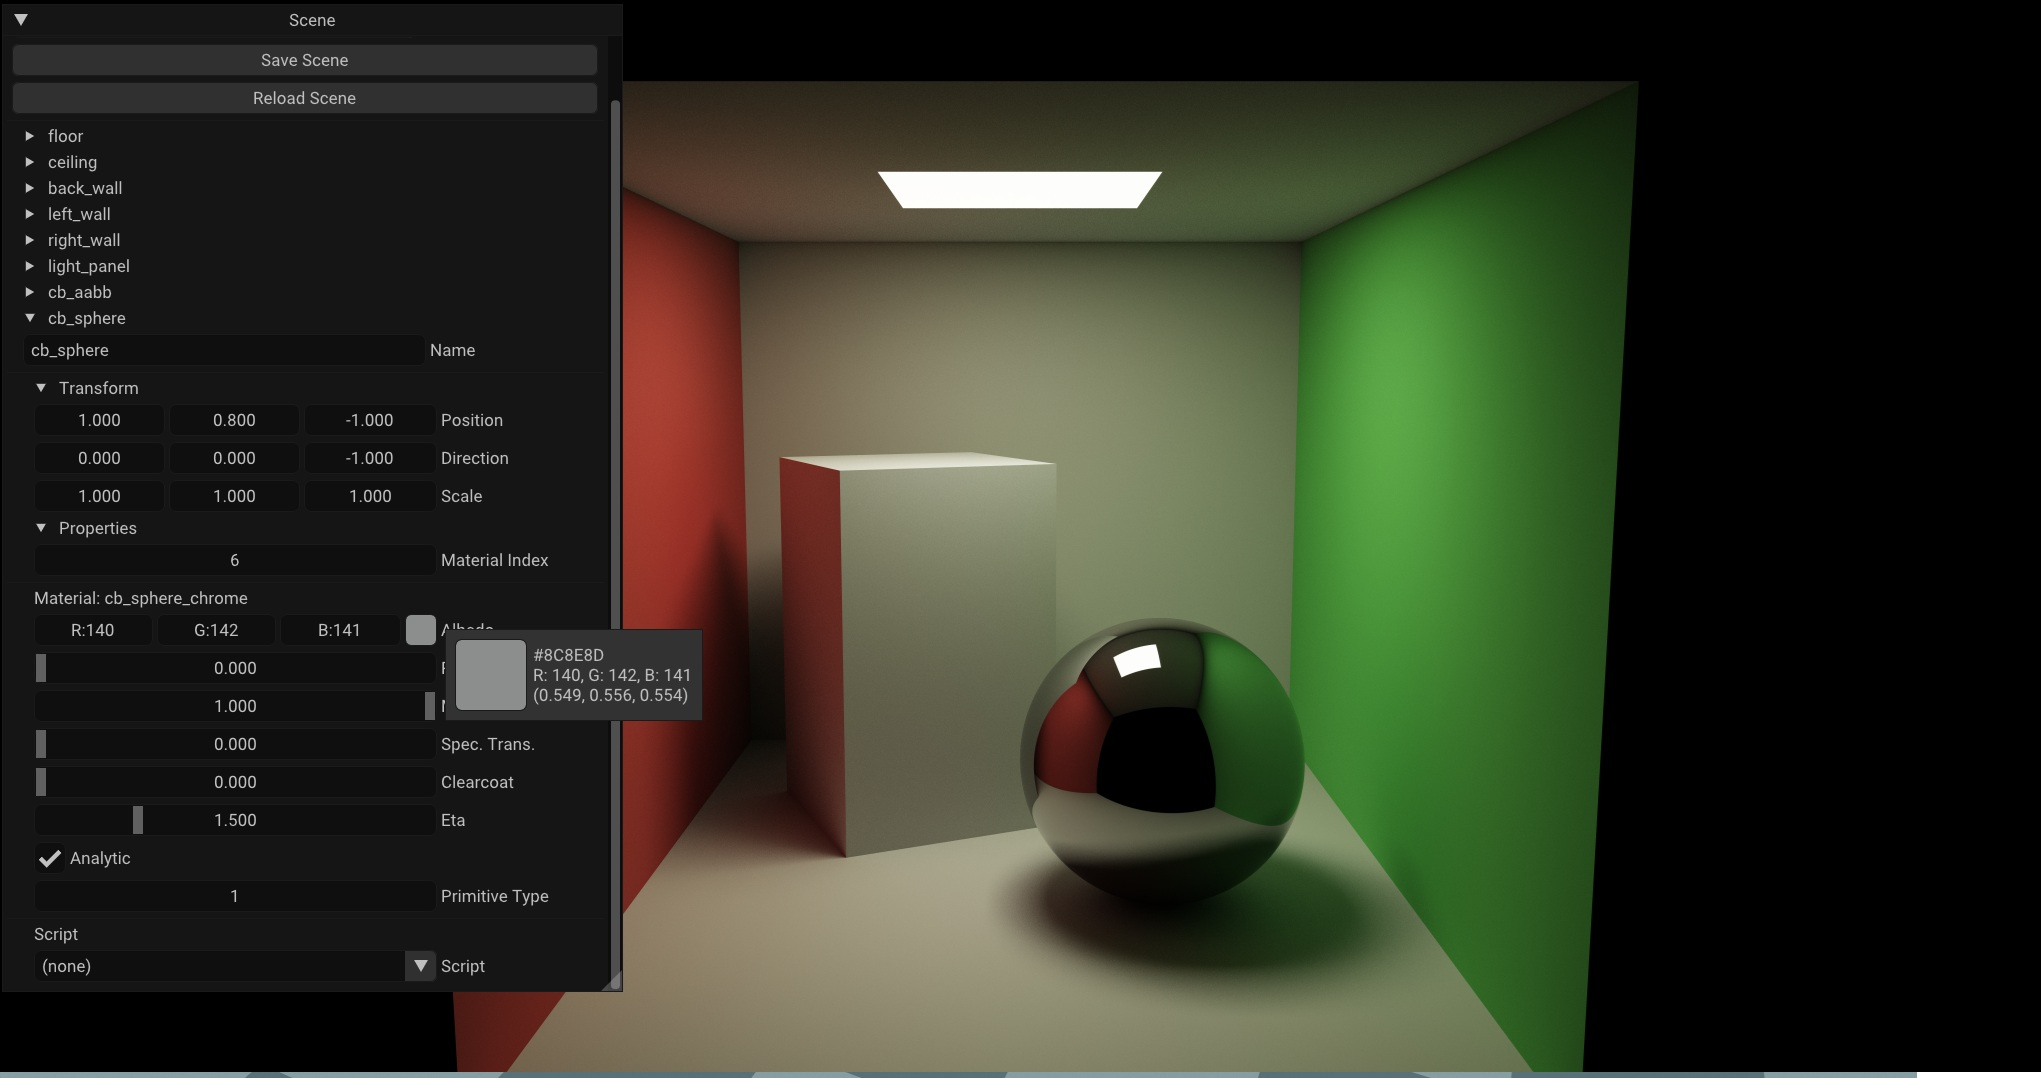
\includegraphics[width=0.9\textwidth]{pics/scene-editor.jpg}
    \caption{Editor de scene în timp real -- vizualizare cu panourile de proprietăți editabile și arborele de entități.}
    \label{fig:scene_editor}
\end{figure}

\section{Rendering}\label{sec:rendering}

Nucleul grafic al proiectului este un motor de Path Tracing, algoritmul fiind implementat integral în shader-e, cu ajutorul pipeline-ului de Ray Tracing hardware oferit de Vulkan.

\subsection{Camera}

Sistemul de cameră este implementat în clasa \texttt{Camera}, oferind o proiecție perspectivă și control de tip \textit{first-person}.
Utilizatorul poate naviga folosind tastele WASD pentru translație și mouse-ul pentru rotație (pitch/yaw).
Rotația se realizează numai la apăsarea butonului de click dreapta.
La salvarea unei scene, se stochează datele despre poziția și rotația camerei, pentru a putea face benchmark-uri repetabile.

\subsection{Pipeline de Ray Tracing}\label{sec:pipeline}

Spre deosebire de rasterizarea tradițională, pentru a folosi accelerare hardware pentru Ray Tracing trebuie activată extensia \texttt{VK\_KHR\_ray\_tracing\_pipeline}.
După activare, \texttt{Vlkrt} definește câteva resurse și structuri de date specifice:
\begin{itemize}
    \item \textbf{Acceleration Structures (AS):} Structură arborescentă care organizează geometria scenei pentru a accelera intersecțiile razelor.
        Se folosesc două niveluri de AS:
        \begin{enumerate}
            \item \textbf{Bottom-Level AS (BLAS):} Conține geometria brută a fiecărui mesh (buffer-e de vertex și index).
            \item \textbf{Top-Level AS (TLAS):} Conține instanțe ale BLAS-urilor, fiecare cu propria matrice de transformare, permițând instanțierea eficientă a obiectelor.
        \end{enumerate}
    \item \textbf{Shader Binding Table (SBT):} Structură de date în Vulkan RT care face legătura între razele lansate și grupurile de shadere executate la impact.
        În implementarea curentă, SBT-ul include grupuri pentru \texttt{raygen} (standard + temporal), \texttt{miss} (radiance + shadow), \texttt{closesthit} (triunghi + AABB) și \texttt{intersection} (analitic + SDF).
\end{itemize}

Un \textit{caveat} al implementării este folosirea a 1 BLAS și 1 TLAS, ceea ce este în regulă pentru scene mici și statice, însă ar putea fi partiționat mai bine pe mesh-uri statice și dinamice.
De altfel, implementarea de față reconstruiește aceste structuri în totalitate la fiecare modificare a scenei.

\subsection{Arhitectură}

Clasa \texttt{Renderer} implementează logica de randare pas cu pas în funcția \texttt{Render()}:

\begin{enumerate}
    \item \textbf{Validarea scenei și (re)alocarea resurselor:} la modificarea scenei (mesh-uri, materiale, lumini), renderer-ul invalidează cache-ul și reconstruiește buffer-ele GPU necesare, precum și structurile de accelerație (BLAS/TLAS).
    \item \textbf{Încărcarea datelor în buffer-ele Vulkan:} geometria, materialele, indicii de material, luminile, transformările și datele pentru primitive analitice/SDF sunt serializate în multiple \texttt{VkBuffer} pentru acces din shader-e.
    \item \textbf{Actualizarea descriptorilor:} renderer-ul menține un descriptor set extins (23 binding-uri) care include TLAS, imagini de output/acumulare, buffer-e de scenă, texturi, date pentru AABB și \textit{ghidajele} necesare pentru NRD/FSR.
    \item \textbf{Istoric pentru reproiecție temporală:} pe lângă buffer-ele curente, renderer-ul menține buffer-e pentru geometria și transformările din cadrul anterior (vertecși și AABB transforms), folosite la reconstrucția de \textit{motion vectors} în stadiile de hit.
    \item \textbf{Sincronizare explicită:} înainte și după fiecare etapă (RT, compute NRD, compose, FSR), se emit bariere \texttt{vkCmdPipelineBarrier} pentru tranziții corecte de layout și acces între \texttt{RAY\_TRACING}, \texttt{COMPUTE} și \texttt{FRAGMENT}.
    \item \textbf{Push constants pentru date "hot":} numărul de lumini, toggle-ul \texttt{One Light Sample}, pragul \texttt{Russian Roulette Depth} și \texttt{SceneIndex} sunt trimise prin push constants (16 octeți), evitând acces repetat la UBO pentru parametri citiți frecvent în toate stagiile RT.
\end{enumerate}

Pe parcursul implementării am testat și o variantă mai agresivă de paralelizare (execuție asincronă/overlap între etape compute și restul pipeline-ului), motivată de faptul că utilizarea GPU nu ajungea constant la 100\%.
În practică, această abordare a introdus artefacte temporale vizibile (ghosting, instabilitate pe umbre/reflexii și inconsistențe între frame-uri), în special în interacțiunea dintre datele de ghidaj, reproiecție și denoising.
Din acest motiv, varianta finală a păstrat un flux sincronizat, cu bariere explicite între etape, preferând corectitudinea vizuală și stabilitatea temporală în detrimentul unui potențial câștig de performanță.

Procesul de randare (în shader-e) urmează fluxul standard de Ray tracing:
\begin{enumerate}
    \item \textbf{Ray generation:} două programe \texttt{raygen} coexistă în pipeline (standard și temporal), selectate din SBT în funcție de modul ales din GUI.
    \item \textbf{Traversarea în TLAS/BLAS:} hardware-ul RT găsește intersecția cea mai apropiată pe triunghiuri sau primitive procedurale.
          Această etapă este fixă, neprogramabilă, și este implementată de către driver-ul Vulkan.
    \item \textbf{Closest hit:} dacă se găsește o intersecție cu o suprafață, se calculează shading PBR, eșantionând informat BSDF-ul materialului.
          Față de \texttt{DieXaR}, se adaugă și calculul și scrierea în buffer-ele de ghidaj pentru NRD/FSR.
    \item \textbf{Miss / Shadow miss:} programe dedicate pentru razele care nu lovesc geometrie sau pentru razele de umbră, returnând contribuția de fundal sau vizibilitatea către sursa de lumină.
    \item \textbf{Post-procesare opțională:} NRD (RELAX) și apoi FSR 3 upscaling, în funcție de setările scenei.
\end{enumerate}

\subsection{Implementarea shader-elor}

Shader-ele sunt scrise în \texttt{Slang} și compilate în SPIR-V.
Pipeline-ul RT folosește 8 stadii (2 \texttt{raygen}, 2 \texttt{miss}, 2 \texttt{closesthit}, 2 \texttt{intersection}), iar compoziția rezultatului NRD folosește un shader \texttt{compute} separat.

SBT-ul este organizat pe regiuni (raygen/miss/hit), iar pentru grupurile AABB se folosește record packing pe 4 bytes (\texttt{instanceIndex << 4 | primitiveType}) pentru a reduce traficul de memorie.

\subsubsection{Ray Generation (\texttt{raygen.rgen})}

Acesta este punctul de intrare pentru modul de Path Tracing standard.
Shader-ul:
\begin{itemize}
    \item Generează raze primare folosind eșantionare stratificată (în funcție de spp), cu jitter opțional.
    \item Inițializează \texttt{RayPayload} cu throughput, stare RNG, date pentru recursie și canale auxiliare pentru NRD (normale, roughness, radiance/hit distance, motion, emission etc.).
    \item Lansează \texttt{TraceRay}, acumulează contribuția radiometrică și aplică tonemapping (ACES) + gamma.
    \item Scrie atât imaginea finală, cât și texturile-ghid necesare etapelor ulterioare (NRD și, la nevoie, FSR depth input).
\end{itemize}

Varianta \texttt{raygen\_temporal.rgen} rulează 1 spp per cadru și acumulează temporal în buffer-ul de afișare, ciclând deterministic eșantioanele în interiorul grilei stratificate.
Acumularea se resetează la mișcarea camerei sau poate fi resetată manual din GUI.

\subsubsection{Closest Hit (\texttt{closesthit.rchit})}

Executat la intersecția cu geometria, acest shader realizează partea cea mai complexă a randării.

\paragraph{Interpolarea atributelor}
Spre deosebire de pipeline-ul grafic clasic, aici avem acces doar la indecșii triunghiului lovit (sau, după caz, la SDF-ul/AABB-ul lovit) și coordonatele baricentrice.
Shader-ul accesează manual buffer-ele (\textit{Structured Buffers}) de vertecși și indecși pentru a încărca datele celor 3 vârfuri și a interpola poziția, normala și coordonatele UV.

\paragraph{Shading PBR și recursie}
Logica de shading folosește modelul Disney Principled BSDF (lobi difuz, specular, clearcoat și transmisie), împreună cu:
\begin{itemize}
    \item \textbf{NEE + MIS} pentru iluminare directă.
    \item \textbf{One-light sampling} configurabil din GUI și aplicat automat pentru bounce-urile terțiare.
          Această optimizare asigură eșantionarea unei lumini aleatorii din scenă, în loc de a eșantiona toate luminile, reducând costul pentru bounce-urile adânci, cu contribuție mică la imaginea finală.
    \item \textbf{Ruletă rusească} pentru terminarea probabilistică a căilor (în funcție de contribuția acumulată), cu prag configurabil la runtime.
\end{itemize}

Pentru texturi, implementarea curentă folosește eșantionare explicită la nivel de mip 0, fără selecție adaptivă de LoD.
Jitter-ul rezolvă problema de aliasing la unghiuri extreme.

\subsubsection{Miss Shader (\texttt{miss.rmiss})}

Miss shader-ul returnează contribuția de fundal pentru razele care nu intersectează geometrie, iar \texttt{shadow\_miss.rmiss} modelează cazul de vizibilitate completă către sursa de lumină pentru razele de umbră.
Pentru majoritatea scenelor, shader-ul de miss returnează culoarea negru.
Pentru scena \texttt{pbr\_showcase}, shader-ul de miss este un gradient de fundal, o reprezentare a cerului cu soare prezent (vezi Figura~\ref{fig:skybox}).

\begin{figure}[H]
    \centering
    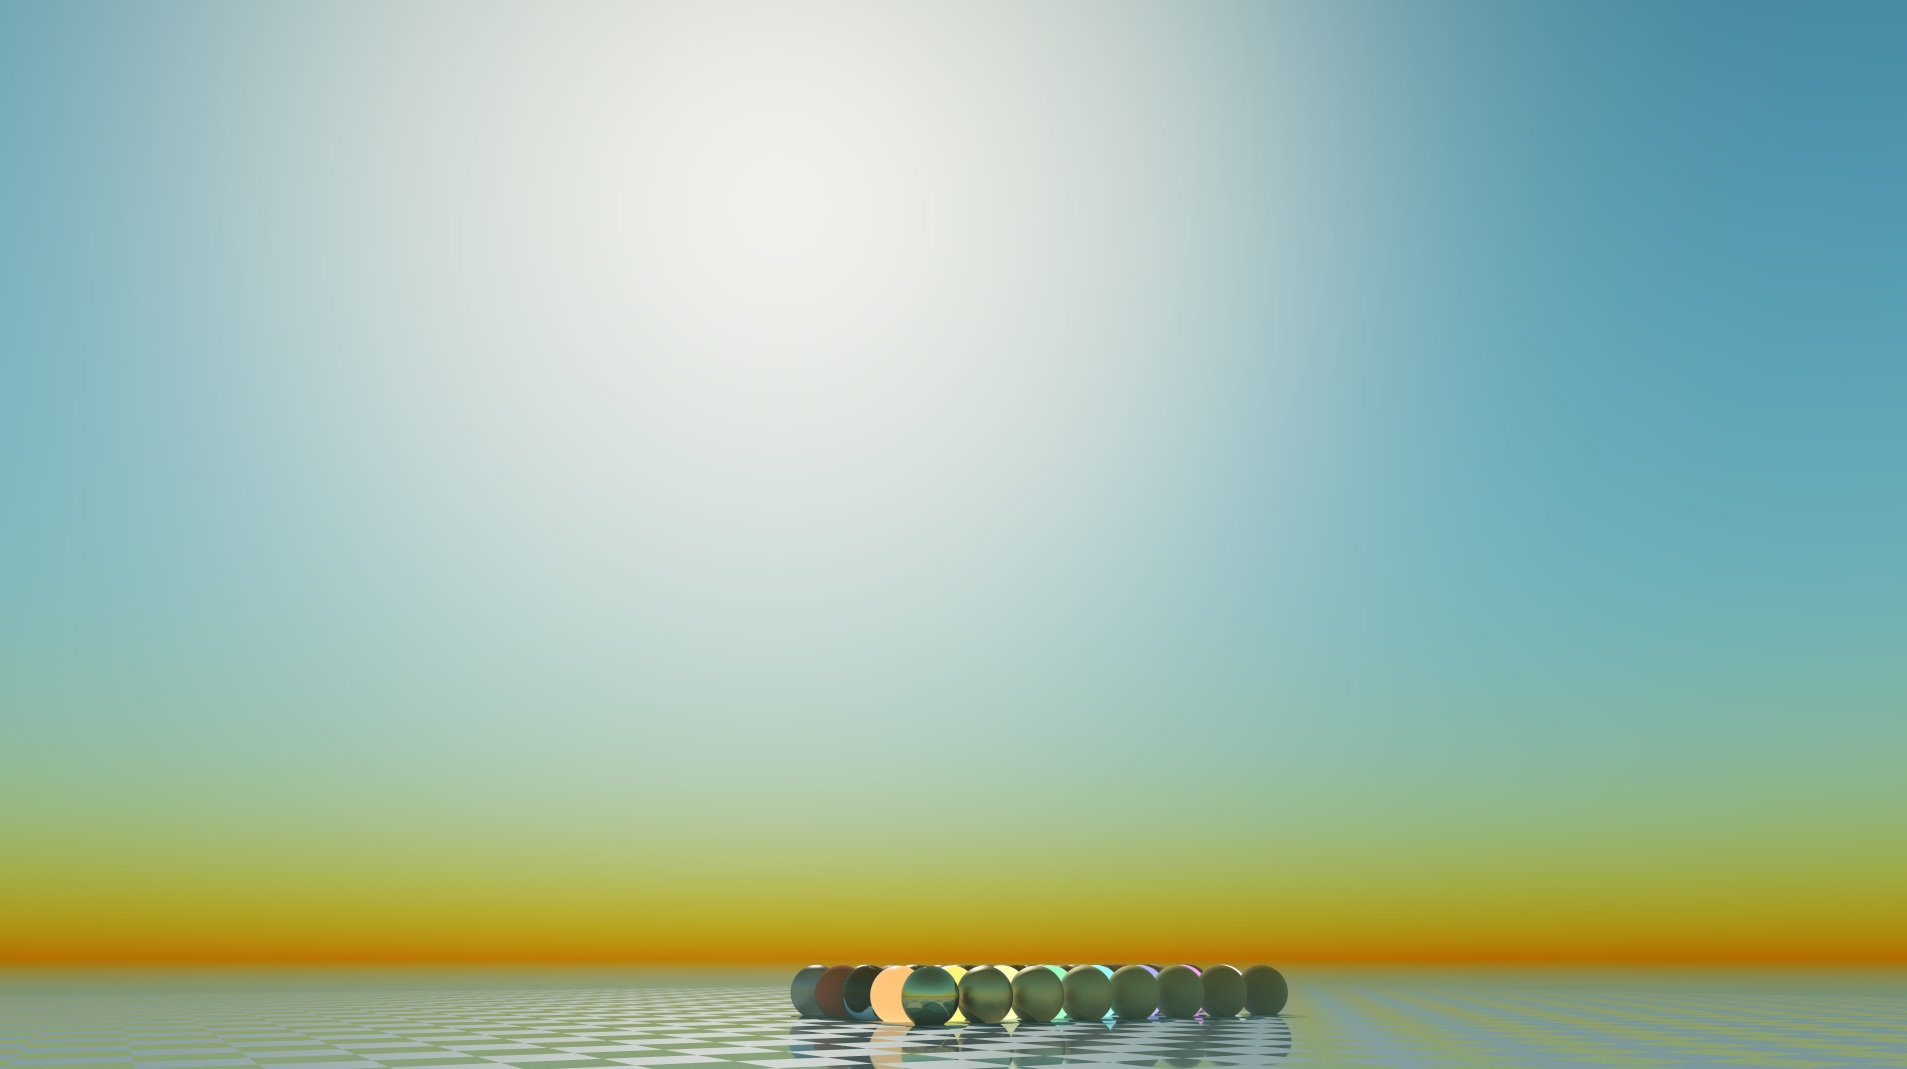
\includegraphics[width=0.9\textwidth]{pics/skybox.jpg}
    \caption{Skyboxul implementat în shader-ul de miss din scena \texttt{pbr\_showcase}.}
    \label{fig:skybox}
\end{figure}

\subsection{Pipeline de Denoising și Upscaling}

Denoising-ul și upscaling-ul sunt implementate în pipeline-uri de compute separate, separat de pipeline-ul de Ray Tracing.
După etapa RT, dacă denoiser-ul NRD este activ, renderer-ul construiește structura de parametri \texttt{NRDDenoiseParams} și execută NRD folosind SDK-ul de la NVIDIA printr-un \texttt{vkCmdDispatch} pe pipeline-ul compute.
Rezultatul este compus peste imaginea finală printr-un pass \texttt{compose\_denoised.comp}.

În plus, implementarea expune în GUI atât buffer-ele de ghidaj (\textit{normal+roughness}, \textit{viewZ}, \textit{motion vectors}, \textit{diffuse/specular radiance+hit distance}), cât și parametrii modificabili pentru RELAX (istoric, prepass blur, anti-lag, praguri de dezocluziune), astfel încât comportamentul temporal al denoiser-ului poate fi ajustat fără restartul aplicației.

Dacă FSR este activ, aplicația calculează rezoluția internă în funcție de \texttt{QualityMode}, aplică jitter Halton pe proiecție și rulează \texttt{ffxDispatch} (din FidelityFX SDK) folosind, drept input, buffer-ele de culoare, adâncime și \textit{motion vectors}.
Această integrare permite combinarea unui Path Tracer zgomotos la 1 spp cu denoising temporal și upscaling spațio-temporal într-un pipeline unificat, controlabil complet din interfața de utilizator.
Rezultatele se îmbunătățesc semnificativ, așa cum se poate vedea în secțiunea de \textit{Evaluare calitativă}~\ref{sec:evaluare_calitativa}.

\section{Scripting}\label{sec:scripting}

Pentru a oferi flexibilitate în simulare, a fost integrat motorul de scripting \texttt{Lua}.
S-a utilizat biblioteca \texttt{sol2} ca wrapper C++ peste \texttt{LuaJIT}, oferind o performanță ridicată și o sintaxă clean pentru bind-uri.
Entitățile din scenă sunt expuse către script-uri, permițând modificarea transformărilor sau a proprietăților materialelor la runtime (e.g., animația \texttt{cube\_animation.lua} din Listarea~\ref{lst:cube_animation}).
Proprietățile expuse includ:
\begin{itemize}
    \item \textbf{Transform:} Conține poziția (\texttt{vec3}), rotația (\texttt{quat}), și scalarea (\texttt{vec3}) a entității.
          Modificările sunt automat aplicate la entitate.
    \item \textbf{Operatori glm:} Bindings pentru calcule cu vectori (operații de adunare, scădere, normalizare, produs scalar) și cuaternioni (rotații, interpolare).
    \item \textbf{Input:} Funcții pentru polling-ul input-urilor utilizatorului.
    \item \textbf{Funcții de bibliotecă standard:} Accesul la bibliotecile Lua standard (\texttt{math, os, table}) pentru logică complexă.
    \item \textbf{Logging:} Binding către metoda de logging din \texttt{Walnut}, bazată pe \texttt{spdlog}\footnote{\url{https://github.com/gabime/spdlog}. Accesat 14.06.2026.}.
\end{itemize}

Ciclul de viață al unui script este următorul:
\begin{enumerate}
    \item La prima actualizare a unei entități cu script, script-ul este încărcat din fișierul \texttt{.lua} și o funcție \texttt{OnUpdate(entity, dt)} este căutată.
    \item La fiecare frame, această funcție este apelată cu entitatea și intervalul de timp \texttt{ts} ca parametri.
    \item Script-ul poate modifica transformările sau alte proprietăți ale entității în mod direct.
\end{enumerate}

\begin{lstlisting}[caption={\texttt{cube\_animation.lua} - Exemplu de script de animație.}, label={lst:cube_animation}, frame=single]
-- cube_animation.lua - Exemplu script de animatie
-- Roteste cubul pe axa Y si aplica oscilatie verticala

local startTime = os.clock()
local initialPos = nil

function OnUpdate(entity, dt)
    local time = os.clock() - startTime

    if initialPos == nil then
        initialPos = vec3.new(entity.Transform.Position.x, entity.Transform.Position.y, entity.Transform.Position.z)
    end

    -- Rotation: rotate around Y axis (0, 1, 0)
    local rotationSpeed = 1.0
    entity.Transform.Rotation = AngleAxis(time * rotationSpeed, vec3.new(0, 1, 0))

    -- Up and down movement: sine wave on Y axis
    local bounceHeight = 1.0
    local bounceSpeed = 2.0
    entity.Transform.Position.y = initialPos.y + math.sin(time * bounceSpeed) * bounceHeight
end
\end{lstlisting}


\chapter{\label{sec:evaluare}Evaluare}

\section{Deployment de server}

În primul și în primul rând, pentru a evalua aplicația, avem nevoie de un server care să ruleze și să fie accesibil.
Acest server poate fi rulat local, prin Docker, construind sistemul de fișiere și apoi rulând un container care expune portul necesar pentru conexiuni:

\begin{lstlisting}[language=bash]
 $ docker build -t vlkrt-server .
 $ docker run --rm -p 1337:1337/udp vlkrt-server 
\end{lstlisting}

Ne vom putea conecta apoi cu un client care rulează pe aceeași mașină, introducând adresa \texttt{localhost:1337}.

Pentru a putea conecta clienți de pe mașini diferite, avem nevoie de un server la distanță, cu portul 1337 expus și accesibil.
Am folosit platforma \texttt{Unikraft Cloud}\footnote{\label{ftn:unikraft}\url{https://unikraft.com}. Accesat 14.06.2026.} pentru a rula serverul într-un microVM, obținând o adresă publică care poate fi folosită de clienți pentru conexiune.
Instrucțiunile de deploy se află în README-ul\footnote{\url{https://github.com/nurof3n/vlkrt/blob/main/README.md}. Accesat 14.06.2026.} proiectului.
Un alt avantaj al acestui scenariu este semantica de \textit{scale-to-zero} pe care o oferă Unikraft Cloud -- atunci când nu există conexiuni deschise către server, platforma salvează un snapshot al stării curente și oprește microVM-ul, economisind resurse.
Când un client încearcă să se conecteze, microVM-ul este restaurat la starea salvată în mai puțin de 10ms, oferind o experiență de conectare aproape instantanee.

\section{\label{sec:evaluare_calitativa}Evaluare calitativă}

Evaluarea calitativă urmărește \textit{calitatea vizuală percepută} a imaginii finale și stabilitatea acesteia în timp, \textbf{nu} viteza de execuție.
În mod concret, în acest subcapitol analizăm nivelul de zgomot rezidual, stabilitatea temporală în scene statice și dinamice, păstrarea detaliilor fine și corectitudinea reconstrucției în zone cu dezocluzii.
Nu vom lua în calcul imagini create cu mai mult de 1 eșantion per pixel din cauza scăderii dramatice a performanței.
Analiza se va concentra în special pe efectul setărilor de acumulare temporală, denoising și upscaling.

\subsection{Comparații vizuale}

Începem cu o comparație vizuală în scena Cornell Box.
Această scenă oferă în particular o convergență lentă și stresează algoritmul de Path Tracing, deoarece singura sursă de iluminare este o lumină de tip suprafață, ce oferă zone întunecate, umbre \textit{soft} și pune la încercare capacitatea renderer-ului de a elimina fenomenul de \textit{fireflies}.

Figura~\ref{fig:qual_cornell_baselines} compară patru configurații de bază: \textit{raw} (fără NRD/FSR), NRD, FSR \textit{Native AA} și NRD + FSR \textit{Native AA}.
Acestea se pot compara mai departe cu imaginea de referință, obținută prin acumulare temporală (fără NRD/FSR) din Figura~\ref{fig:qual_cornell_accum}.
Observațiile principale sunt:
\begin{itemize}
    \item Fără NRD, zgomotul la 1 spp rămâne dominant, mai ales în umbrele de contact și pe suprafețele glossy; se observă foarte multe artefacte de tip \textit{fireflies} pe suprafețele difuze ale pereților.
    \item Activarea NRD reduce semnificativ zgomotul perceput și stabilizează umbrele mari, netezind suprafețele difuze; totuși, pe suprafața metalică a sferei se amplifică fenomenul de \textit{fireflies} care era prezent pe pereți.
    \item FSR în modul \textit{Native AA} aduce anti-aliasing util, jucând și un rol parțial de denoiser -- acesta face să pară că imaginea a fost randată cu mai multe eșantioane per pixel.
    \item Combinația NRD + FSR \textit{Native AA} oferă cele mai clare suprafețe difuze, însă încă suferă de zgomot alb pe suprafața metalică a sferei.
\end{itemize}

\begin{figure}[htb]
    \centering
    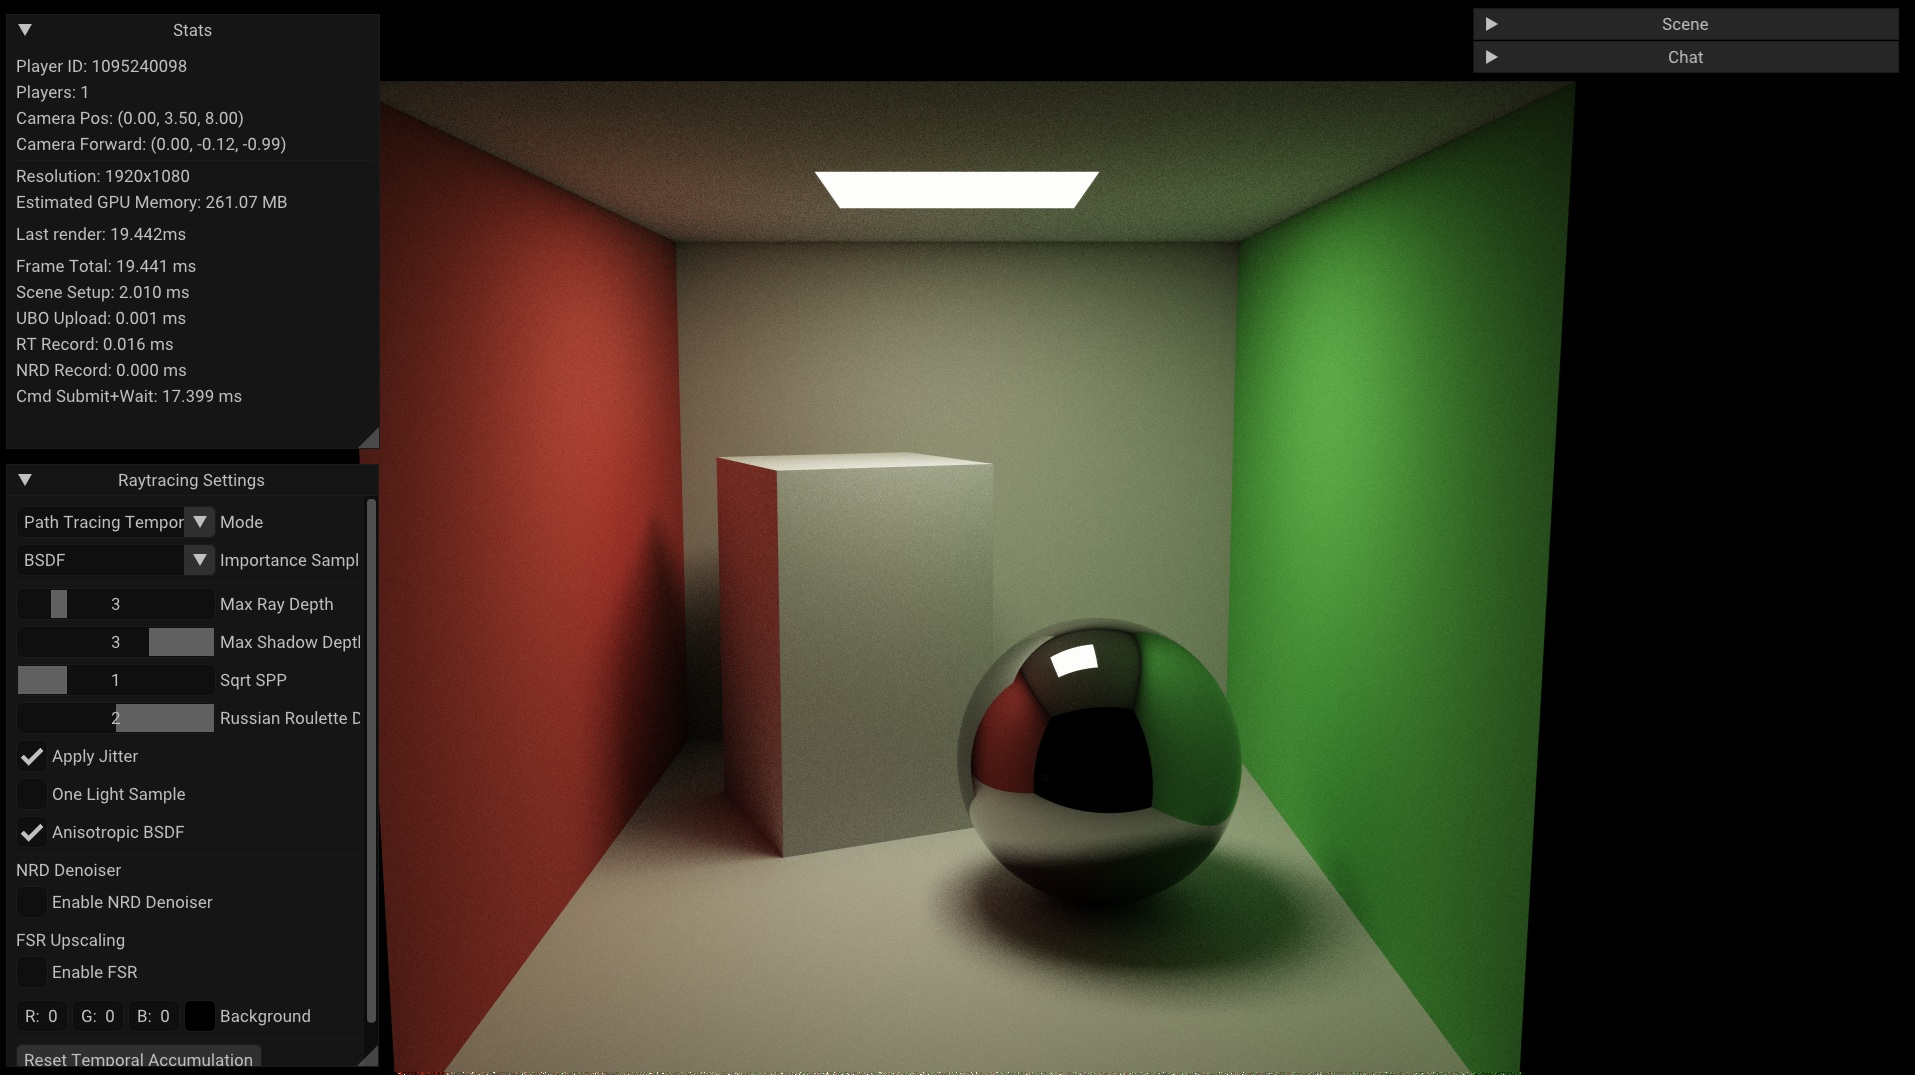
\includegraphics[width=0.9\textwidth]{pics/cornell-box-accum.jpg}
    \caption{Imagine de referință pentru Cornell Box, obținută prin acumulare temporală la 1 spp fără NRD/FSR.}
    \label{fig:qual_cornell_accum}
\end{figure}

\begin{figure}[htb]
    \centering
    \begin{subfigure}[t]{0.49\textwidth}
        \centering
        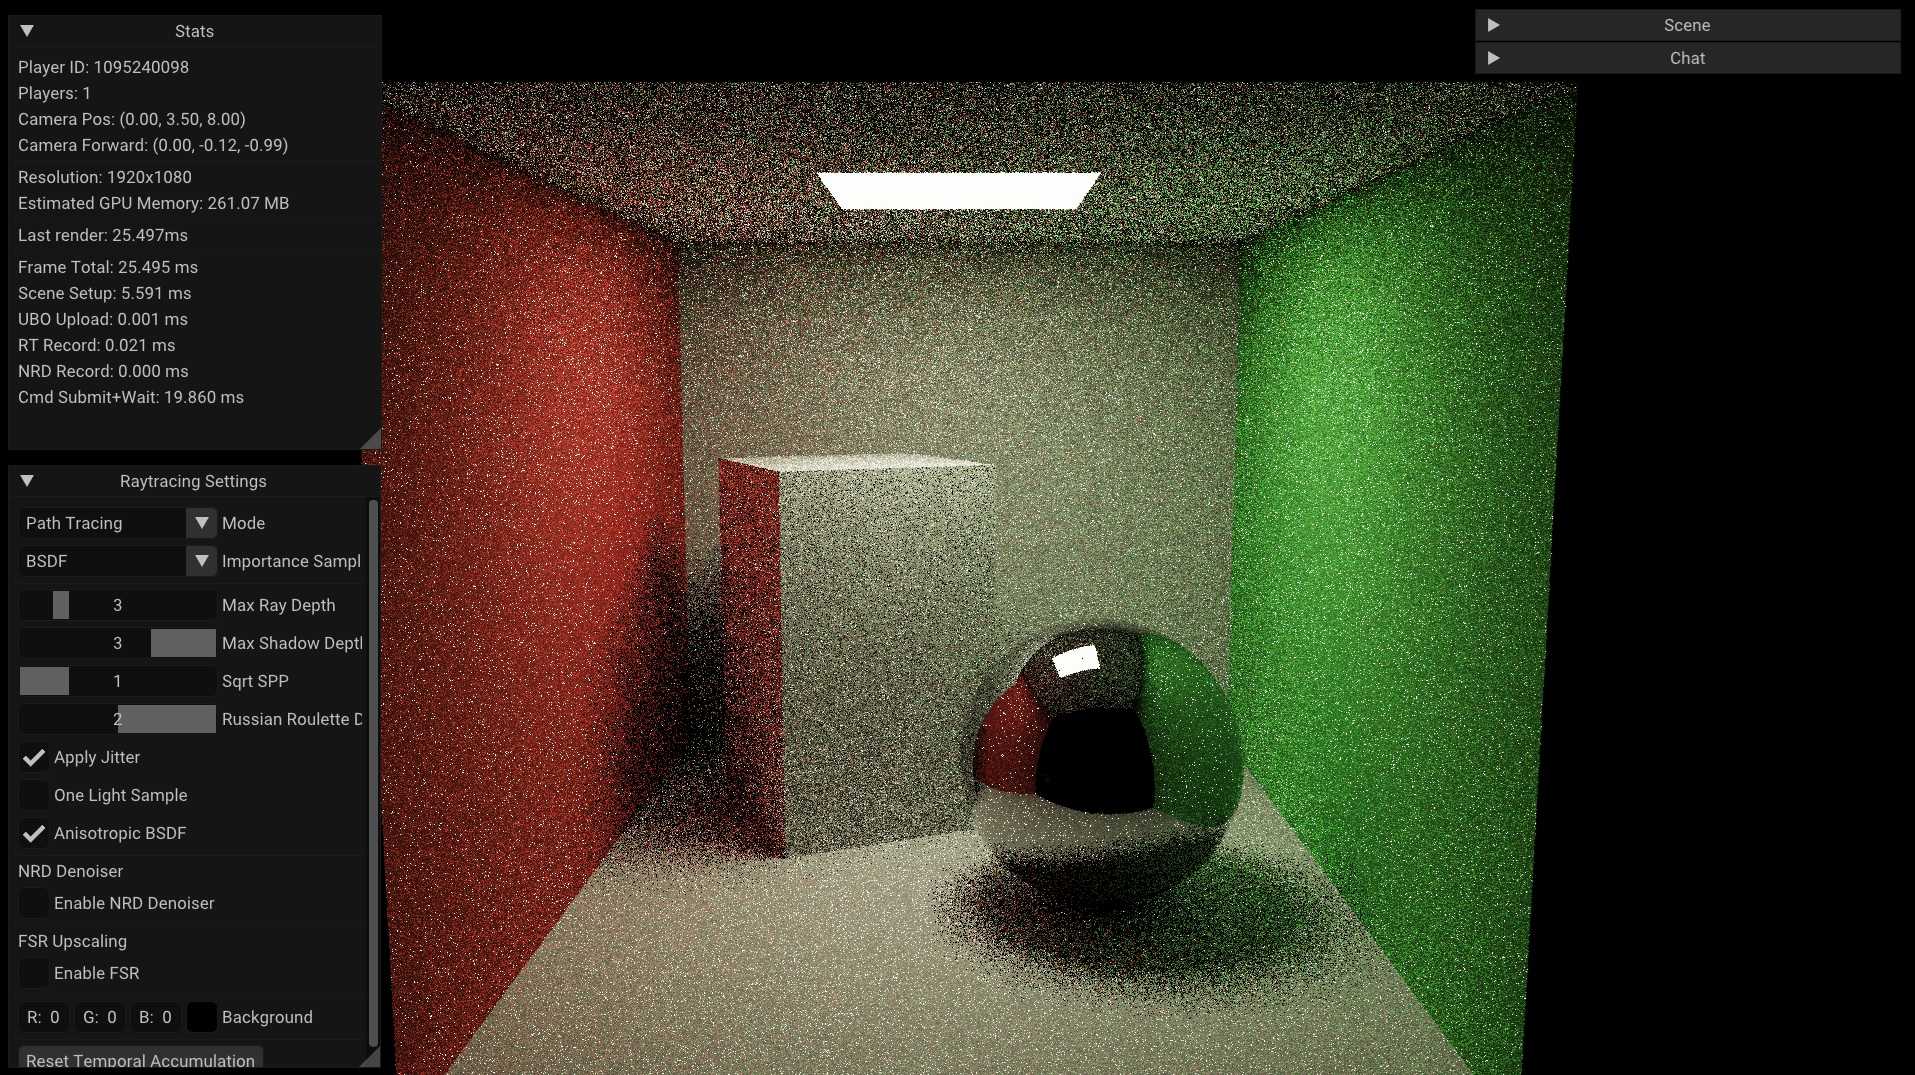
\includegraphics[width=\textwidth]{pics/cornell-box-raw.jpg}
        \caption{Fără NRD, fără FSR (raw)}
    \end{subfigure}
    \hfill
    \begin{subfigure}[t]{0.49\textwidth}
        \centering
        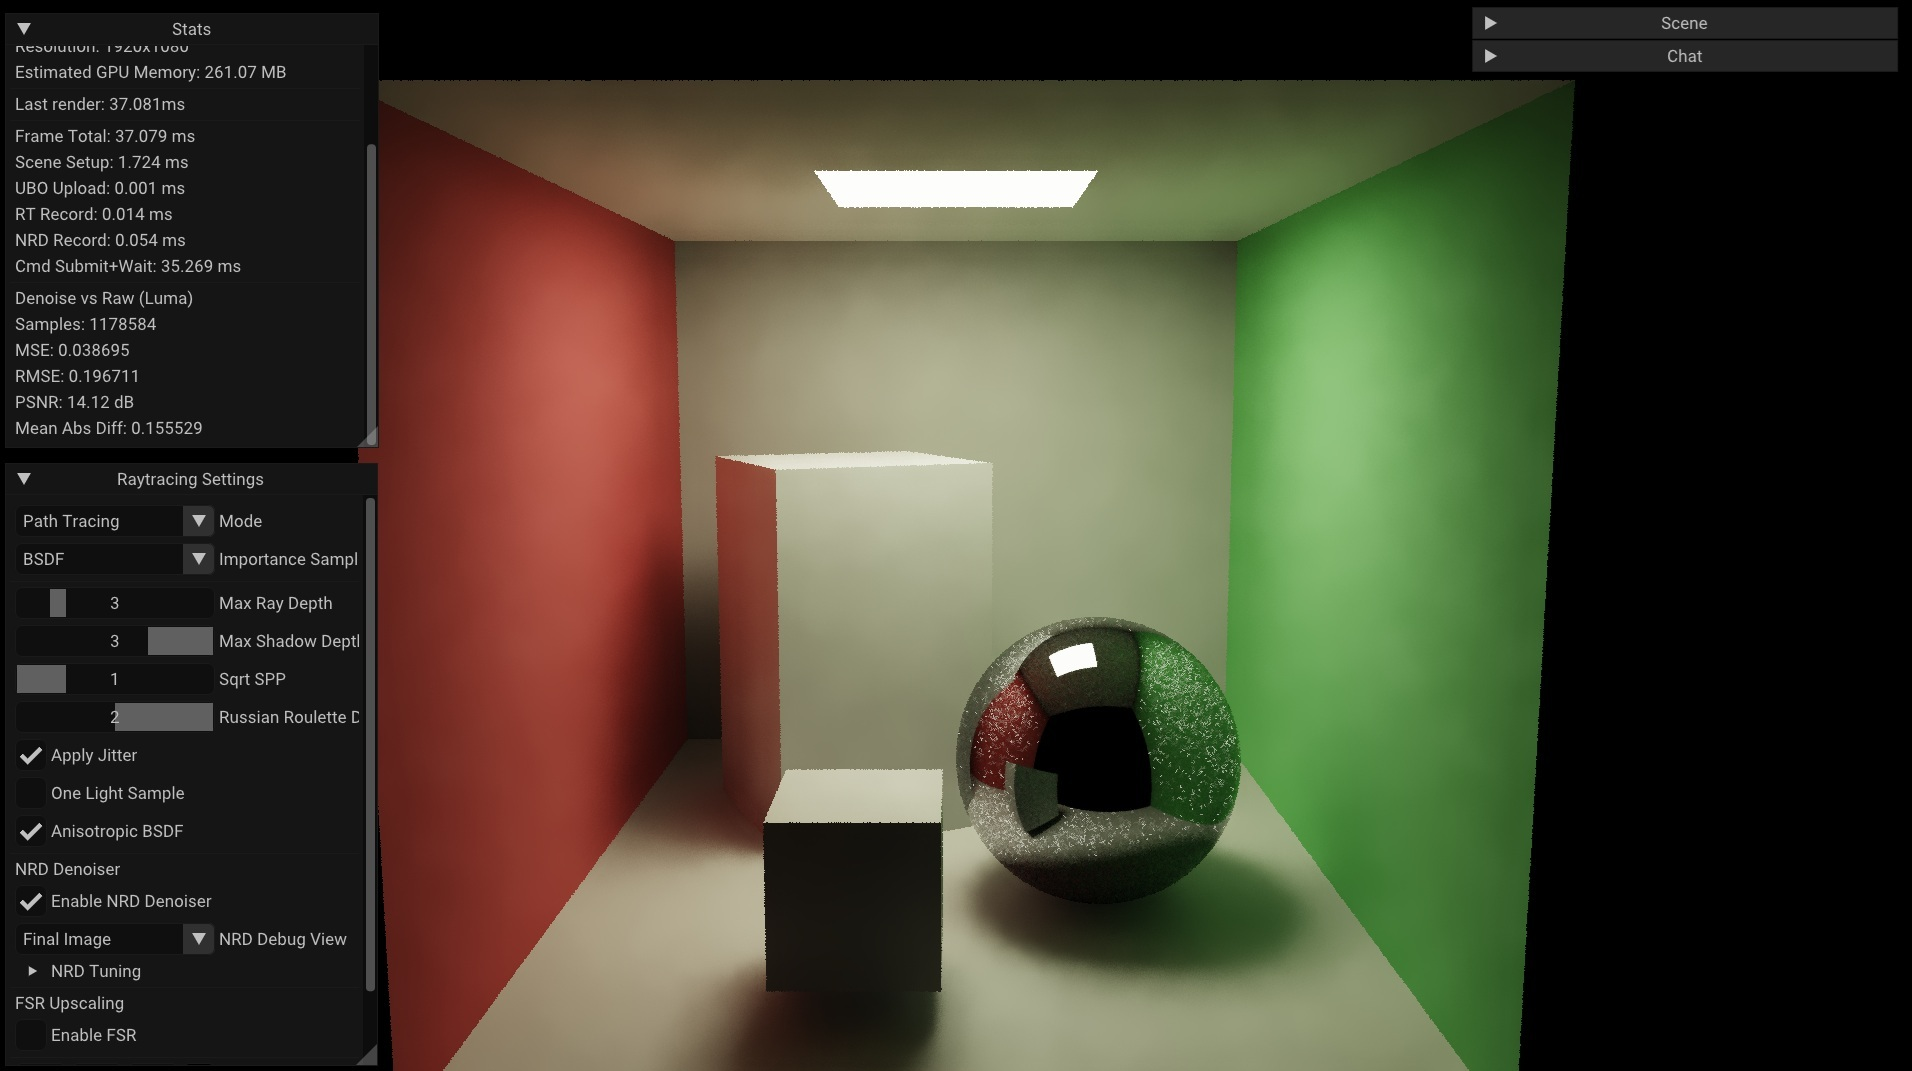
\includegraphics[width=\textwidth]{pics/cornell-box-nrd.jpg}
        \caption{NRD activ, FSR inactiv}
    \end{subfigure}

    \vspace{0.3cm}

    \begin{subfigure}[t]{0.49\textwidth}
        \centering
        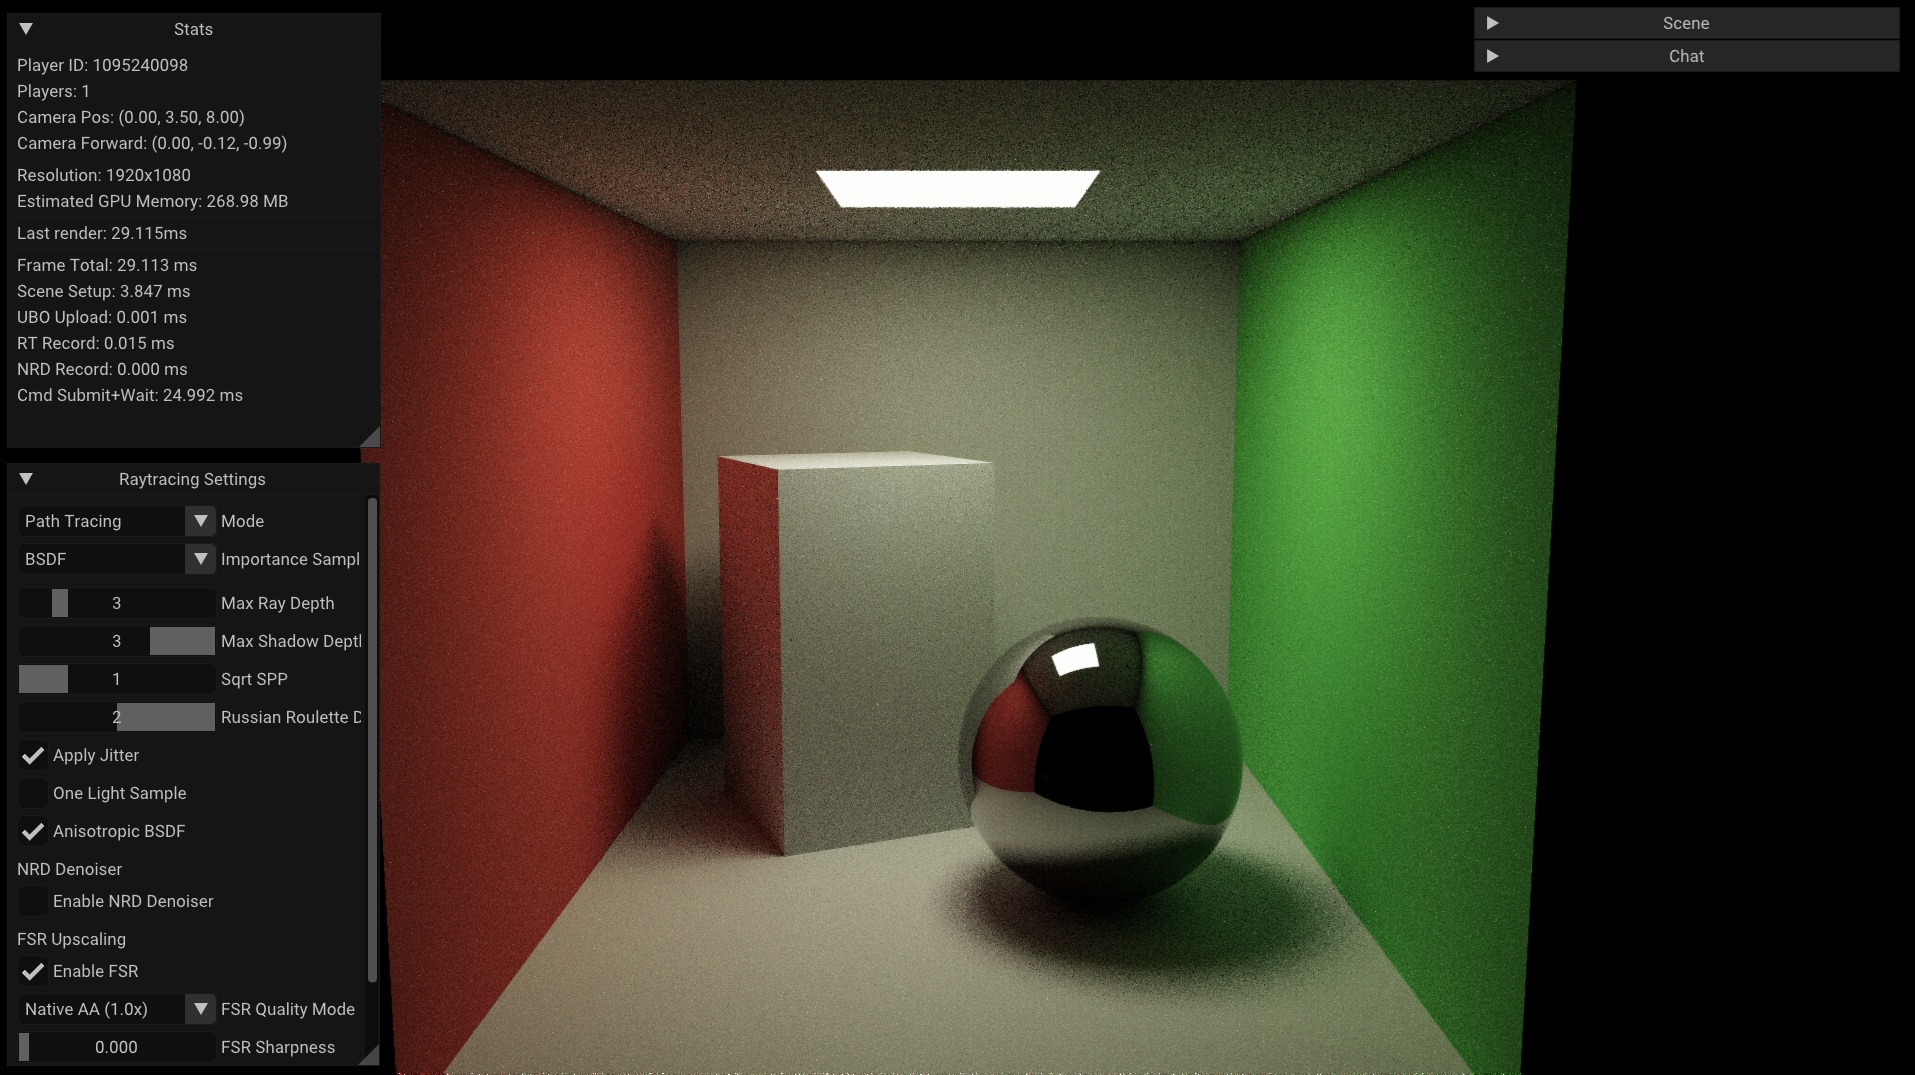
\includegraphics[width=\textwidth]{pics/cornell-box-fsr-aa.jpg}
        \caption{FSR Native AA, fără NRD}
    \end{subfigure}
    \hfill
    \begin{subfigure}[t]{0.49\textwidth}
        \centering
        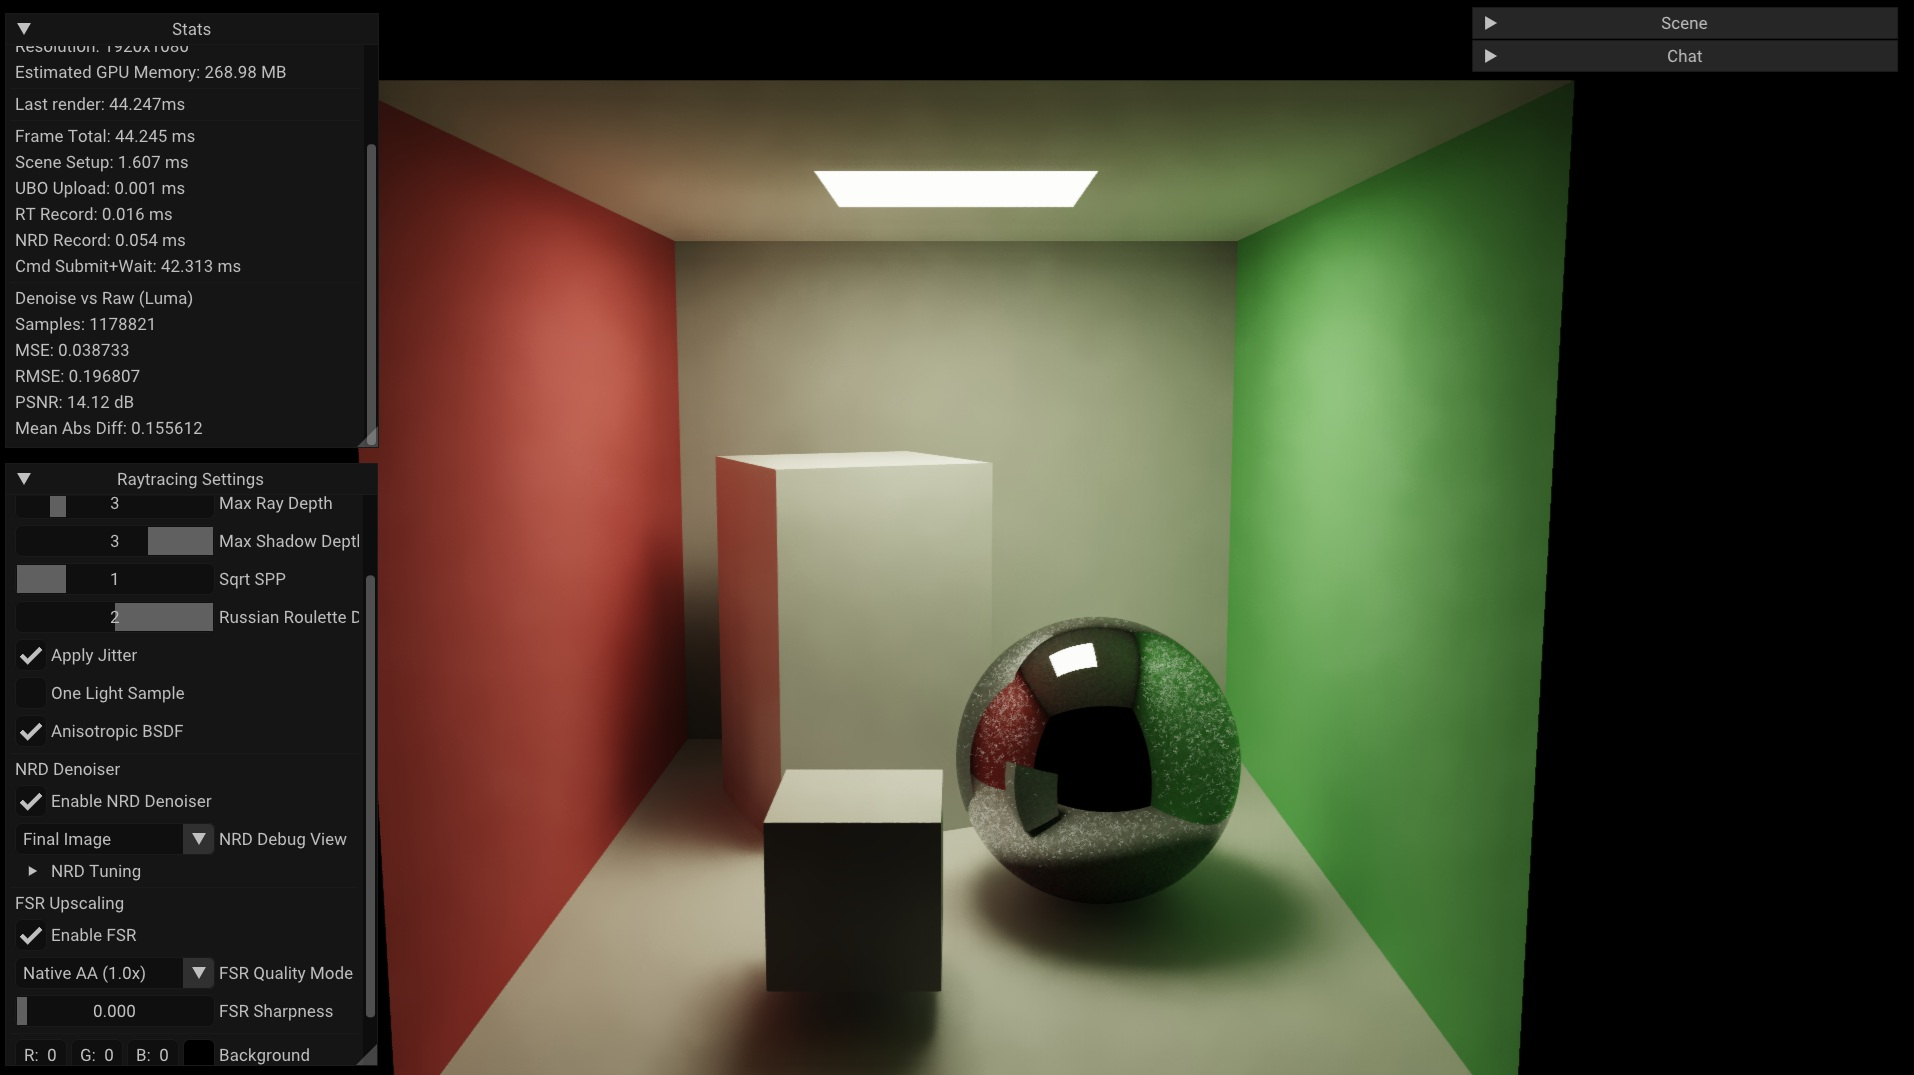
\includegraphics[width=\textwidth]{pics/cornell-box-nrd-fsr-aa.jpg}
        \caption{NRD + FSR \textit{Native AA}}
    \end{subfigure}
    \caption{Comparație vizuală pentru configurațiile de bază în Cornell Box.}
    \label{fig:qual_cornell_baselines}
\end{figure}

Un alt side-effect al denoiser-ului este efectul subtil de \textit{over-brightening} al suprafețelor difuze de pe pereți -- pare că aceștia primesc mai multă lumină.

Figura~\ref{fig:qual_cornell_fsr_modes} arată comportamentul NRD + FSR pe modurile de upscaling.
În \textit{Quality} și \textit{Balanced} se păstrează bine contururile și umbrele, cu detalii acceptabile pe suprafețele glossy.
În \textit{Performance} și mai ales \textit{Ultra Performance}, costul computațional scade puternic, dar apare softening vizibil pe muchii și pierdere de detalii locale.

\begin{figure}[htb]
    \centering
    \begin{subfigure}[t]{0.49\textwidth}
        \centering
        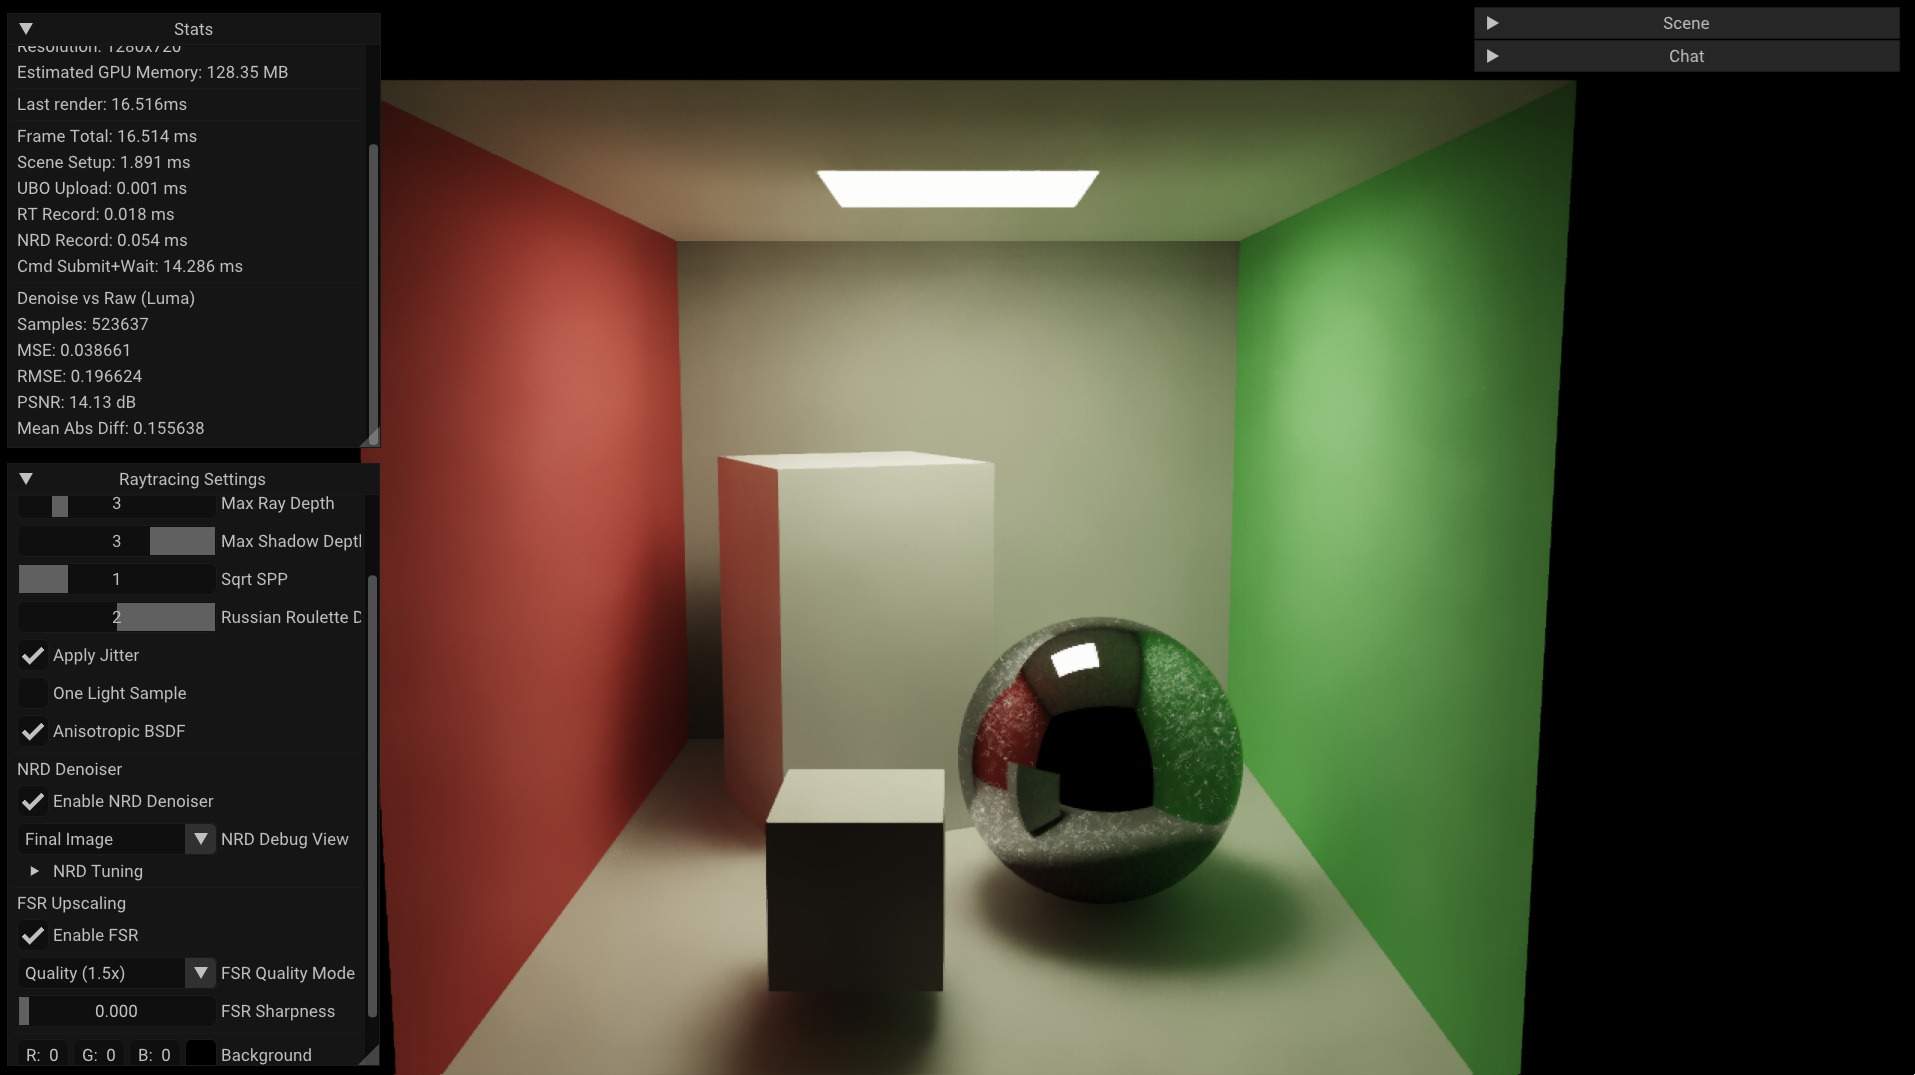
\includegraphics[width=\textwidth]{pics/cornell-box-nrd-fsr-quality.jpg}
        \caption{NRD + FSR Quality (1.5x).}
    \end{subfigure}
    \hfill
    \begin{subfigure}[t]{0.49\textwidth}
        \centering
        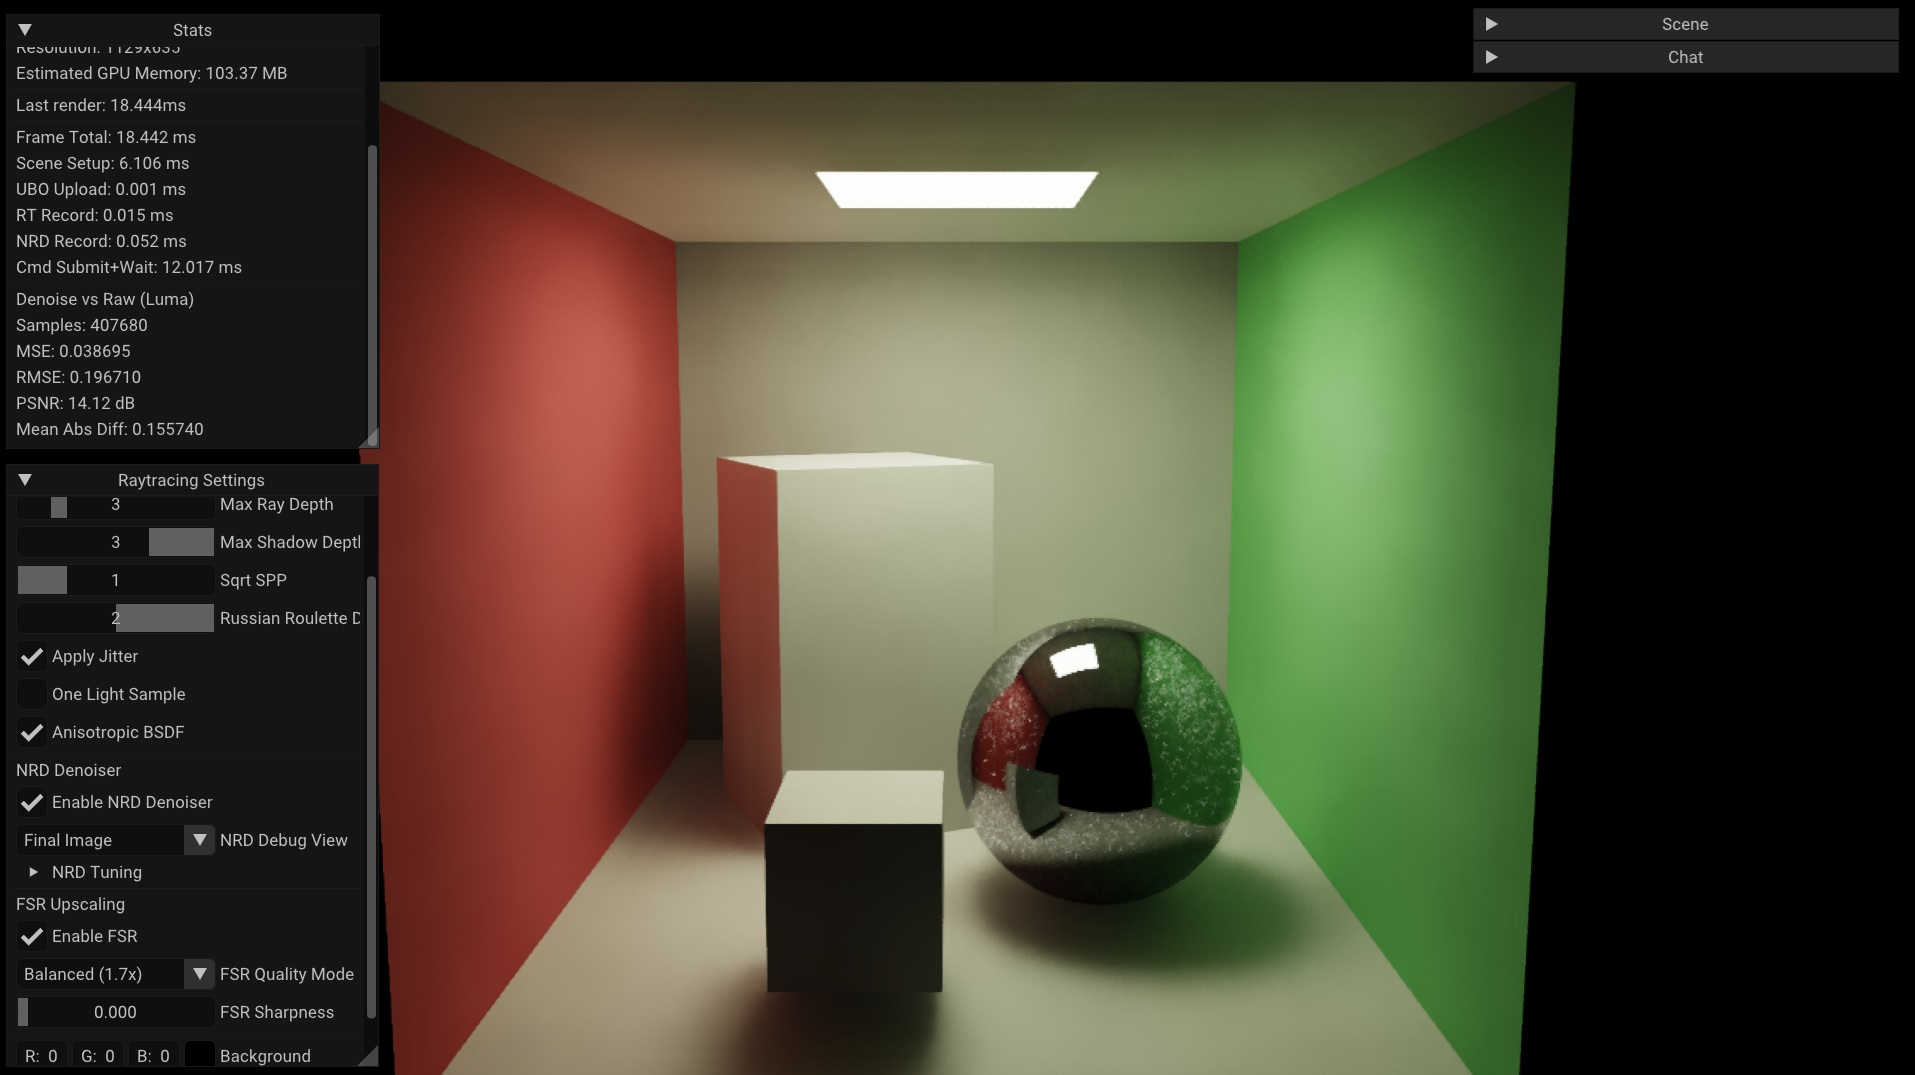
\includegraphics[width=\textwidth]{pics/cornell-box-nrd-fsr-balanced.jpg}
        \caption{NRD + FSR Balanced (1.7x).}
    \end{subfigure}

    \vspace{0.3cm}

    \begin{subfigure}[t]{0.49\textwidth}
        \centering
        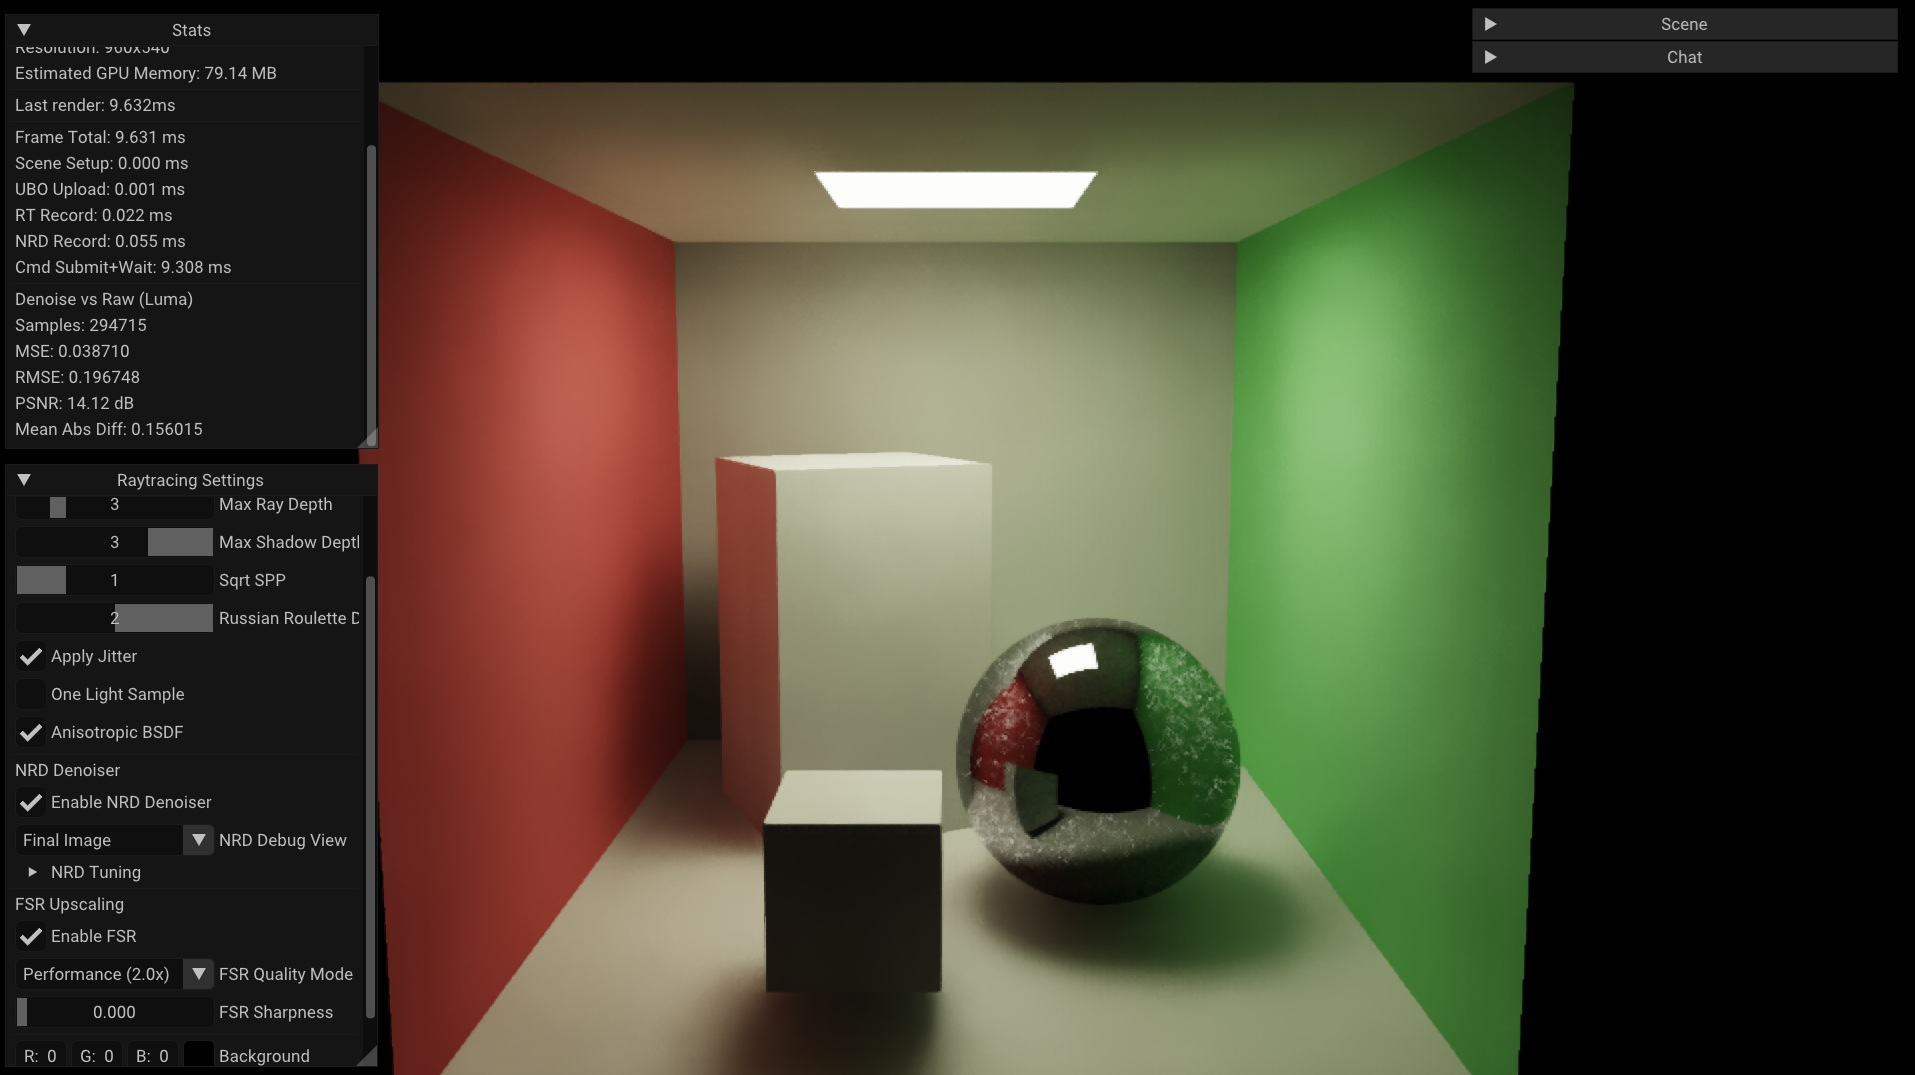
\includegraphics[width=\textwidth]{pics/cornell-box-nrd-fsr-perf.jpg}
        \caption{NRD + FSR Performance (2.0x).}
    \end{subfigure}
    \hfill
    \begin{subfigure}[t]{0.49\textwidth}
        \centering
        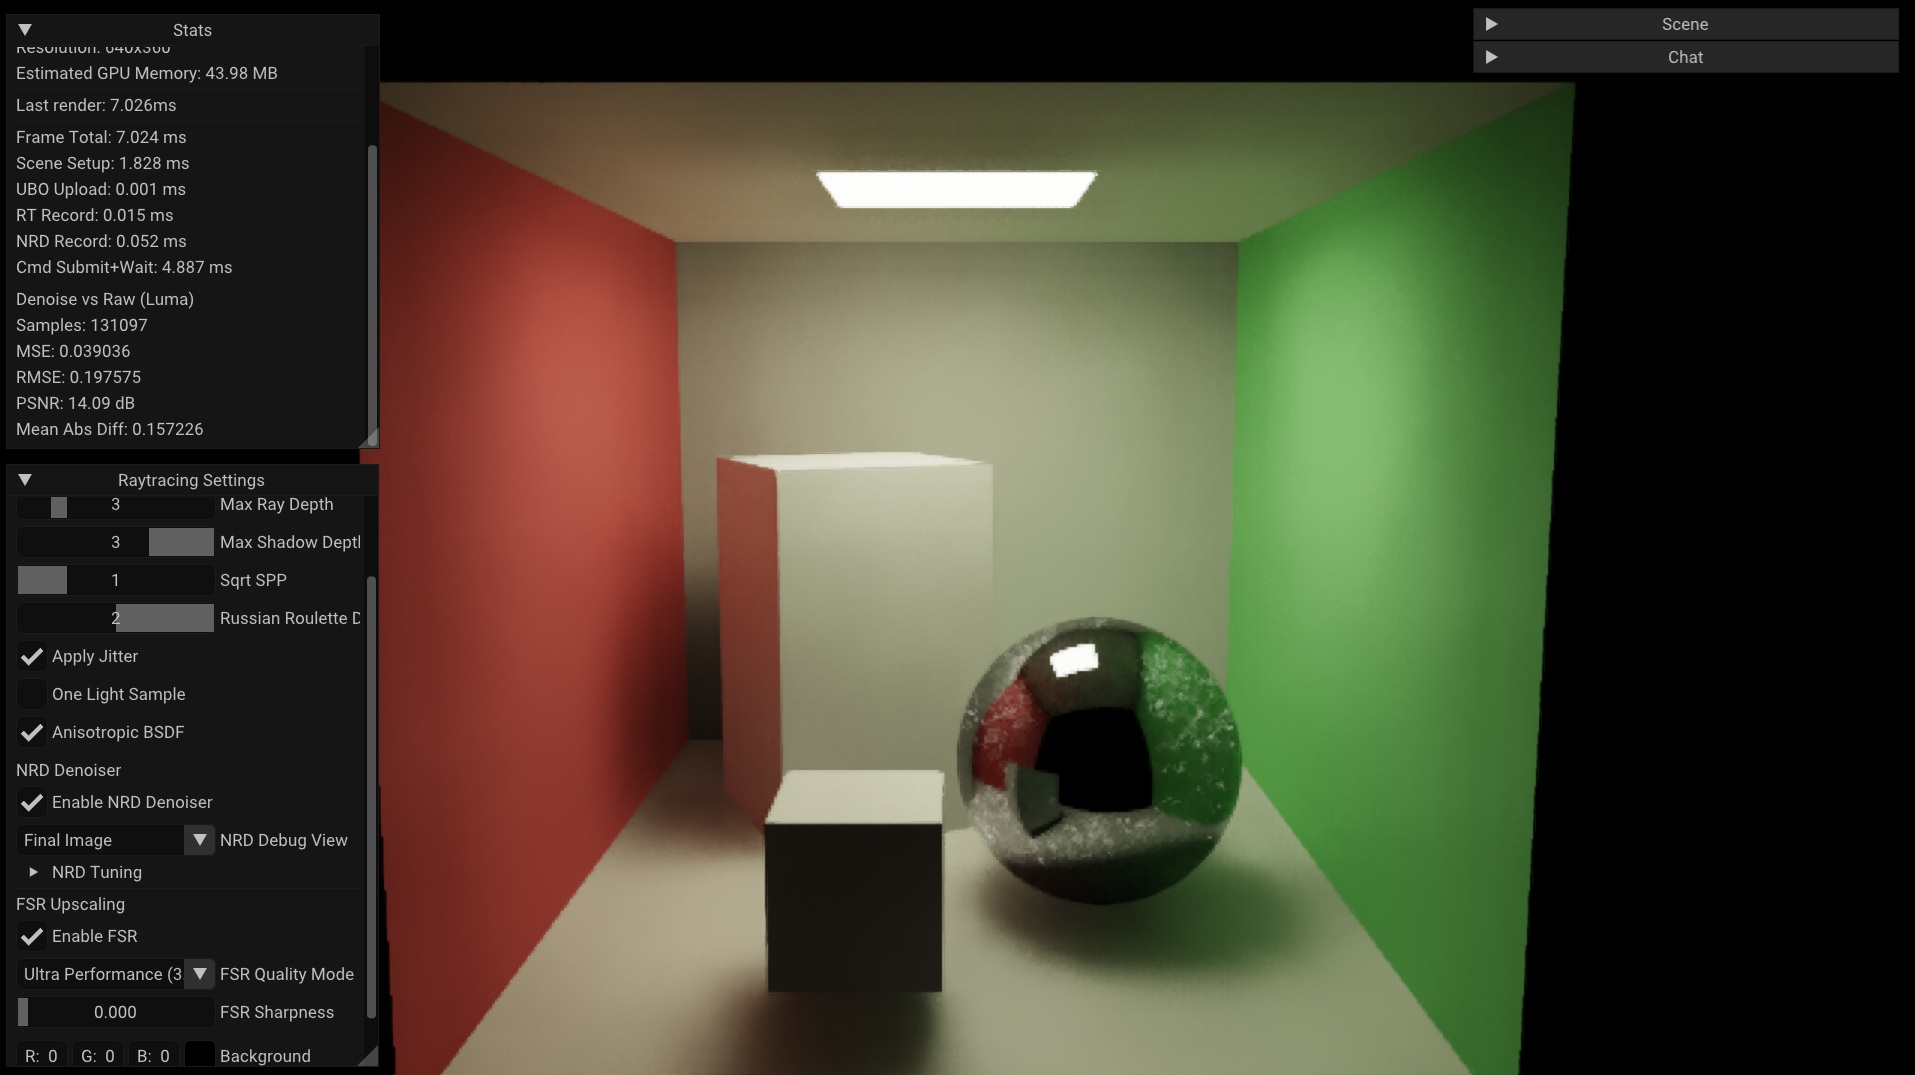
\includegraphics[width=\textwidth]{pics/cornell-box-nrd-fsr-ultraperf.jpg}
        \caption{NRD + FSR Ultra Performance (3.0x).}
    \end{subfigure}
    \caption{Comparație vizuală între modurile FSR, cu NRD activ.}
    \label{fig:qual_cornell_fsr_modes}
\end{figure}

Un parametru care are un impact semnificativ asupra imaginii \textit{raw} este \texttt{One Light Sample}, care limitează Path Tracer-ul la a eșantiona o singură lumină din scenă per bounce.
În scenele cu mai multe lumini de suprafață, precum scena \texttt{demo}, acesta crește performanța, dar adaugă zgomot semnificativ.
Aici denoiser-ul excelează, reușind să elimine complet acest zgomot (vezi Figura~\ref{fig:demo_ols}).

\begin{figure}
    \centering
    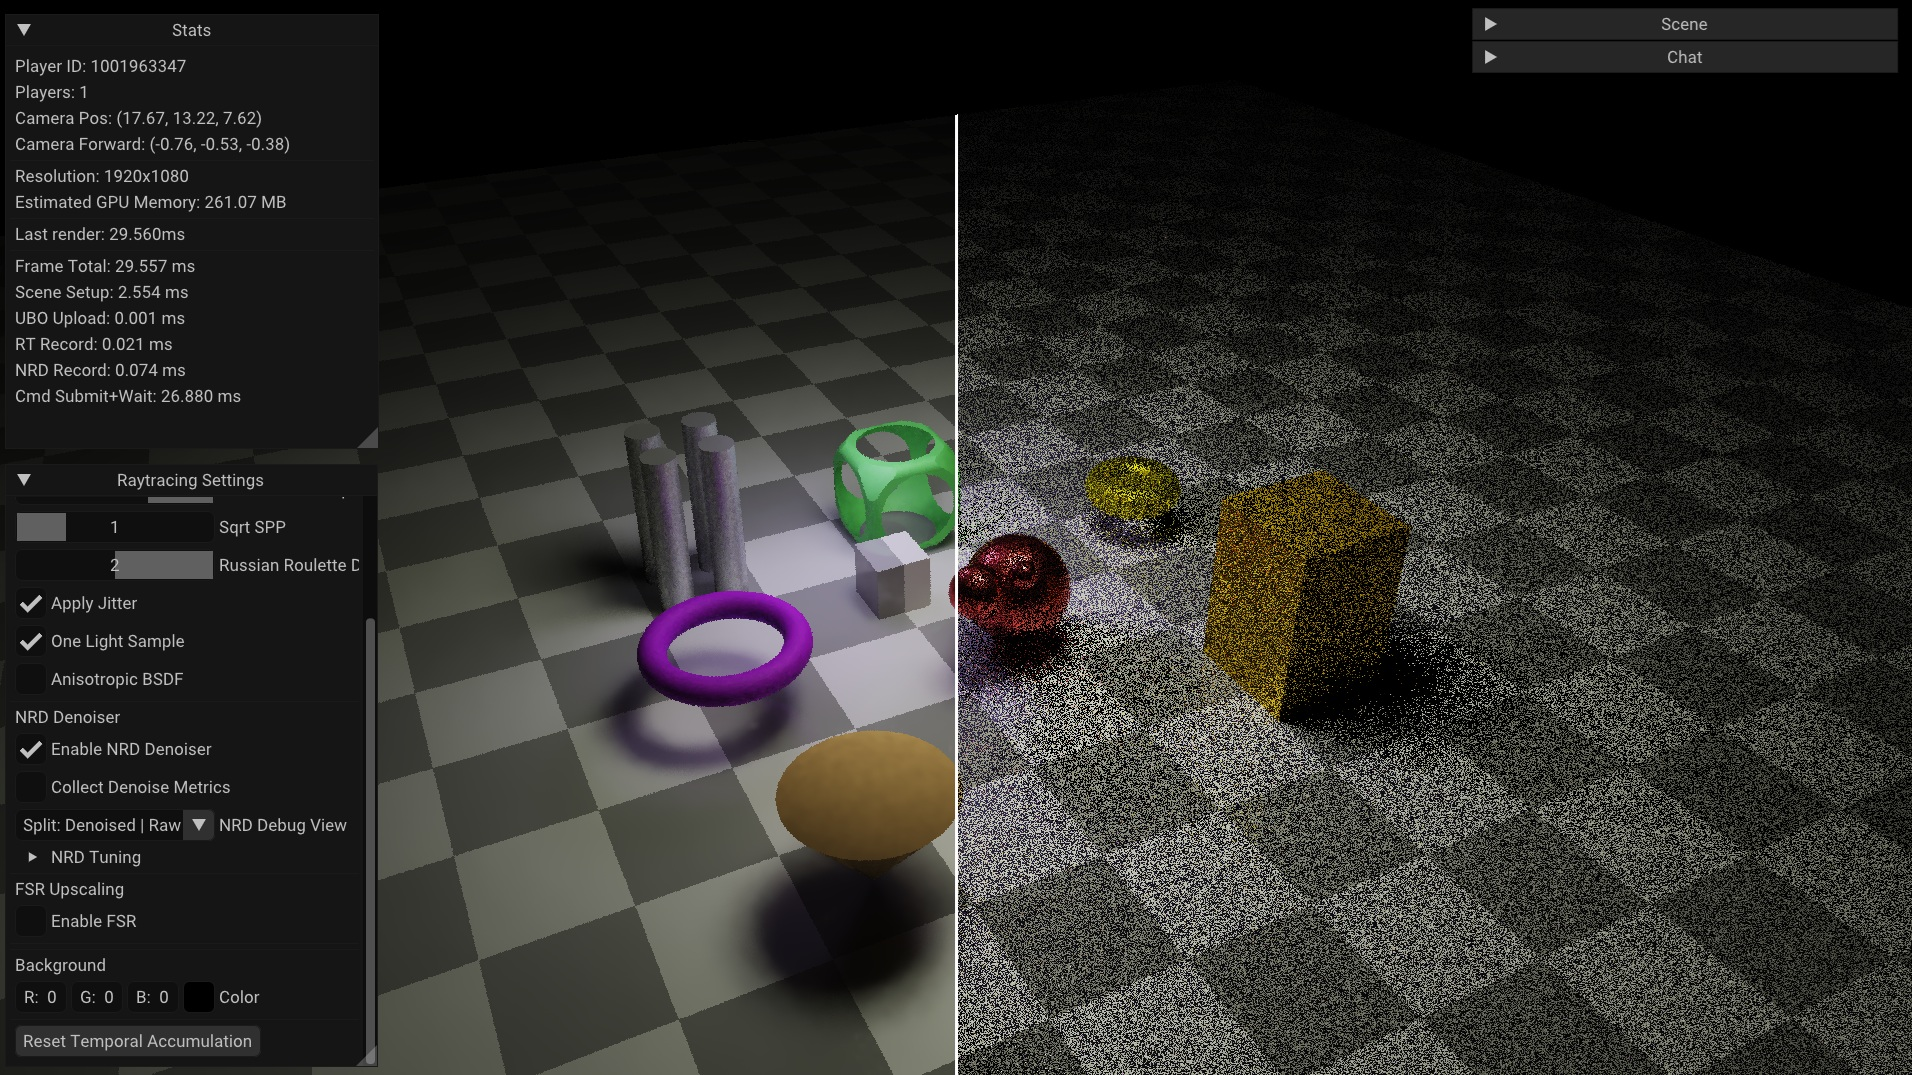
\includegraphics[width=0.9\textwidth]{pics/demo-ols-comparison.jpg}
    \caption{NRD se descurcă de minune la eliminarea zgomotului creat de \texttt{One Light Sample}.}
    \label{fig:demo_ols}
\end{figure}

\subsection{Metrici calitative}

Atunci când NRD este activat, apare un nou toggle în GUI -- \texttt{Collect Denoise Metrics}.
Dacă este activat, apare o secțiune în panoul de statistici cu câteva metrici care să măsoare diferența dintre imaginea denoised și imaginea \textit{raw} sau o imagine de referință.
Pentru a crea acea imagine de referință, se selectează un număr de cadre dorit și se apasă butonul \texttt{Record Reference}.
În acest moment, motorul începe să randeze, folosing Path Tracing cu acumulare temporală, o imagine de referință, care să fie convergentă.
Când este gata, se va putea vedea că secțiunea nouă din panoul de statistici se numește acum \texttt{Denoised vs Reference}, în loc de \texttt{Denoised vs Raw}.

Valorile oferite de panoul de statistici sunt, în ordine:

\begin{itemize}
    \item \textbf{Samples:} numărul de pixeli validați în compute pass (care nu sunt din fundal), folosiți la agregarea metricilor.
    \item \textbf{MSE (Mean Squared Error):} media pătratelor diferențelor de luma dintre imaginea denoised și imaginea raw. Comparația se face în spațiul imaginii de afișare (după tonemapping ACES și gamma).
    \item \textbf{RMSE (Root Mean Squared Error):} rădăcina pătrată a MSE pentru diferența de luma, în același spațiu de afișare.
    \item \textbf{PSNR (Peak Signal-to-Noise Ratio):} calculat din MSE de luma (în dB), cu referință de vârf 1.0. Valori mai mari înseamnă că rezultatul denoised este mai apropiat de imaginea raw, nu neapărat că este vizual superior.
    \item \textbf{Mean Abs Diff (Mean Absolute Difference):} media valorilor absolute ale diferențelor de luma dintre imaginea denoised și cea raw.
\end{itemize}

În acest context, \textit{luma} reprezintă componenta de luminanță a pixelilor, calculată ca $Y = 0.2126 R + 0.7152 G + 0.0722 B$ și este folosită pentru a evalua diferența dintre imaginea denoised și cea raw.
Este o metrică mai bună decât compararea directă a valorilor RGB, deoarece luma este mai apropiată de percepția vizuală umană.

În Tabela~\ref{tab:qual_nrd_metrics} sunt prezentate aceste metrici pentru diferite configurații de upscaling ale scenei Cornell Box.
Aceste metrici provin din comparația cu o imagine de referință randată prin acumulare temporală de 128 cadre.
Prima intrare din tabel reprezintă o randare \textit{raw}, restul sunt denoised.
Astfel, am demonstrat statistic faptul că denoiser-ul funcționează.
De asemenea, remarcăm faptul că metricile sunt practic invariante față de rezoluția internă a FSR, însă modurile de rezoluție scăzută arată o scădere de aproximativ 0.5\% a PSNR.

\begin{table}[htb]
    \centering
    \small
    \begin{tabular}{lrrrrr}
        \hline
        Configurație & Samples & MSE & RMSE & PSNR (dB) & Mean Abs Diff \\
        \hline
        FSR off & 1178584 & 0.028697 & 0.169403 & 15.42 & 0.118191 \\
        NRD, FSR off & 1178584 & 0.011278 & 0.106200 & 19.48 & 0.095523 \\
        NRD, FSR AA & 1178821 & 0.011276 & 0.106190 & 19.48 & 0.095625 \\
        NRD, FSR Quality & 523637 & 0.011521 & 0.107335 & 19.39 & 0.096707 \\
        NRD, FSR Balanced & 407680 & 0.011483 & 0.107157 & 19.39 & 0.096900 \\
        NRD, FSR Performance & 294715 & 0.011645 & 0.107911 & 19.34 & 0.097527 \\
        NRD, FSR Ultra Performance & 131097 & 0.012087 & 0.109940 & 19.18 & 0.099751 \\
        \hline
    \end{tabular}
    \caption{Metricile calitative calculate în scena Cornell Box.}
    \label{tab:qual_nrd_metrics}
\end{table}

\subsection{Artefacte temporale}

Fiind algoritmi temporali, NRD și FSR pot introduce în mod natural artefacte de tip \textit{ghosting}.
Am analizat acest fenomen pe scena \texttt{demo}, făcând capturi de ecran în timp ce un cub se mișcă pe diagonala spațiului de vizualizare, din stânga sus în dreapta jos.
Figura~\ref{fig:qual_demo_ghosting} ilustrează trei situații relevante în acest sens:
\begin{itemize}
    \item \textbf{FSR fără NRD}: cubul lasă în urma sa un \textit{trail}, demonstrând ghosting accentuat în scenele cu mult zgomot.
          Putem observa faptul că obiectele statice acumulează informație temporală, care reduce zgomotul, în timp ce cubul rămâne zgomotos din cauza informației de reproiecție limitată.
    \item \textbf{FSR + NRD}: zgomotul scade vizibil, dar cubul tot lasă urme pe traiectoria de mișcare.
          Și umbra acestuia este afectată.
    \item \textbf{FSR + NRD + One Light Sample}: Deoarece randarea originală suferă de zgomot substanțial cu această setare, informația temporală este greu de refolosit în mișcare.
          Se poate observa faptul că umbra cubului rămâne în urma sa mai mult decât în celelalte scenarii.
\end{itemize}

Aceste cadre confirmă că, în scene dinamice cu dezocluzii și umbre de contact, NRD/FSR îmbunătățesc semnificativ stabilitatea globală,
dar nu elimină complet artefactele temporale, în special când datele de \textit{motion vectors} sau semnalul de lumină directă variază abrupt de la un cadru la altul.

\begin{figure}[htb]
    \centering
    \begin{subfigure}[t]{0.32\textwidth}
        \centering
        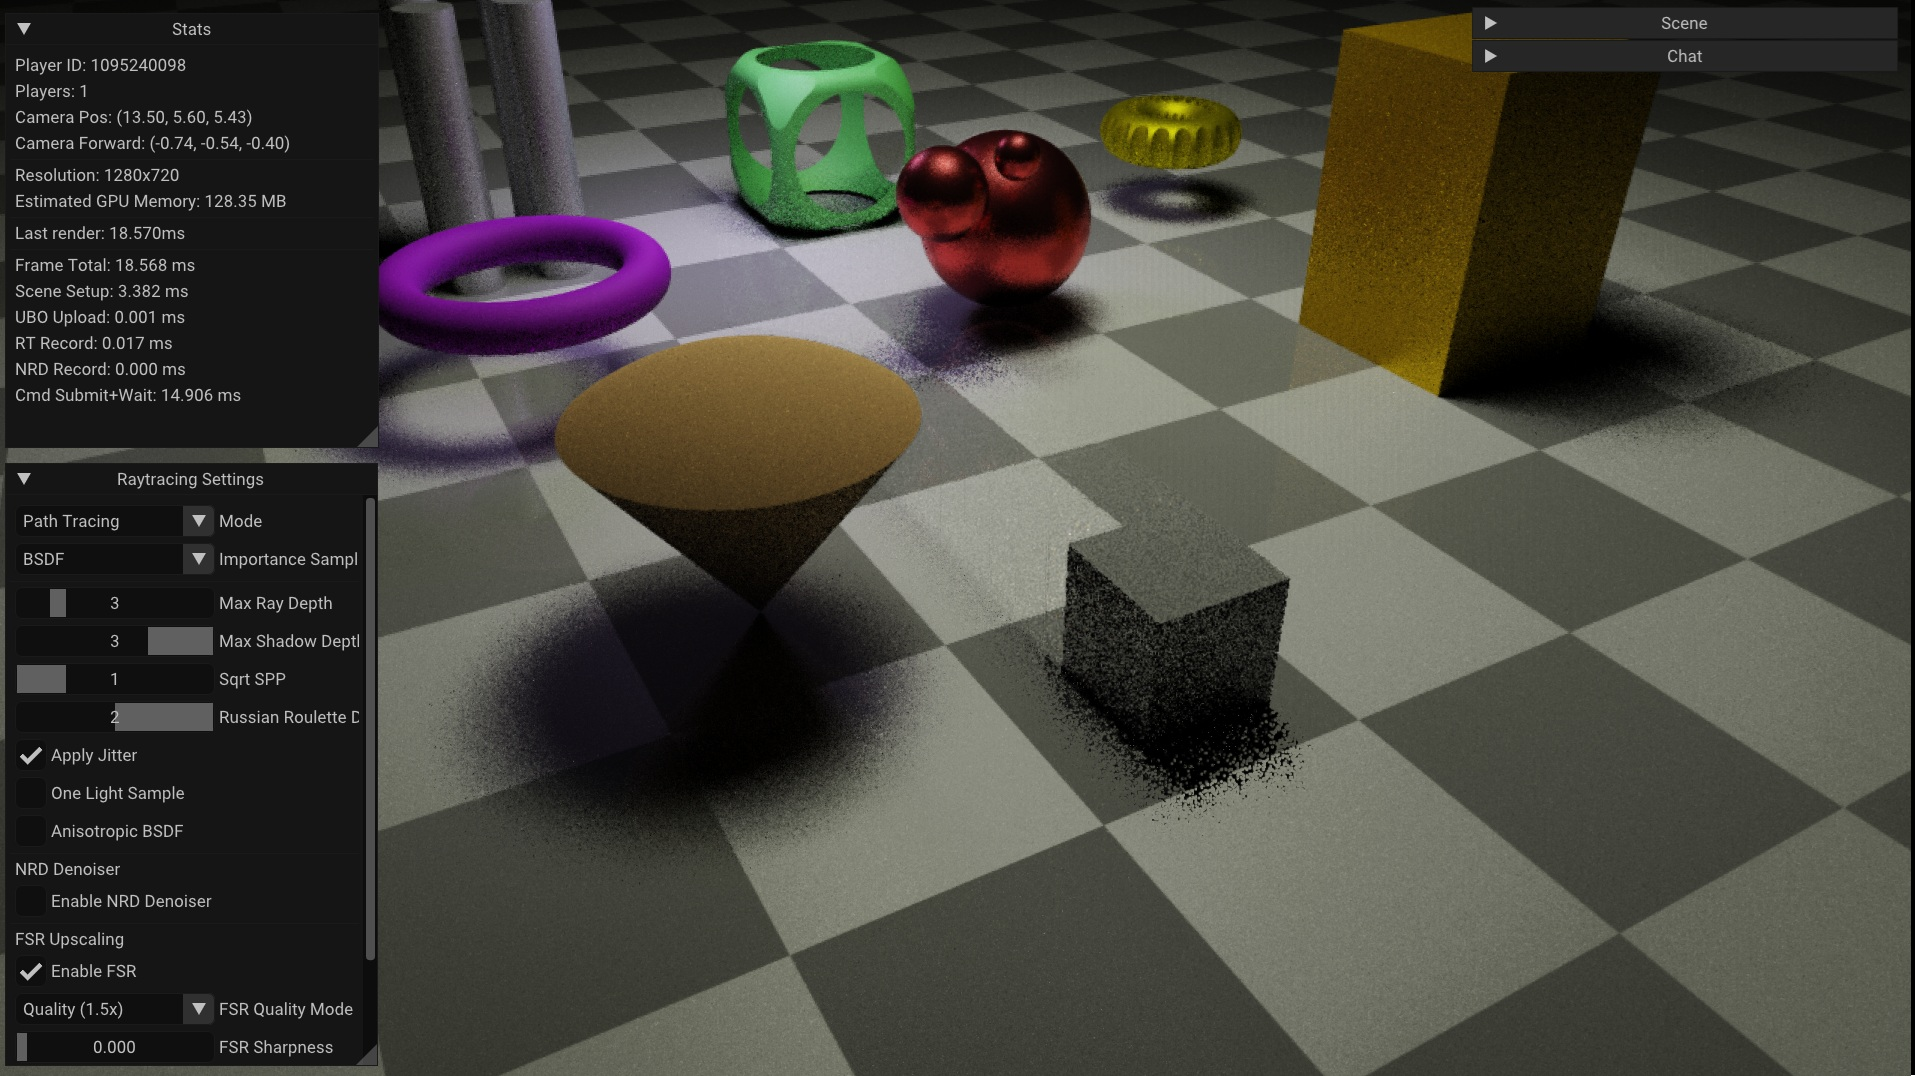
\includegraphics[width=\textwidth]{pics/demo-fsr-ghosting.jpg}
        \caption{FSR activ, NRD inactiv.}
    \end{subfigure}
    \hfill
    \begin{subfigure}[t]{0.32\textwidth}
        \centering
        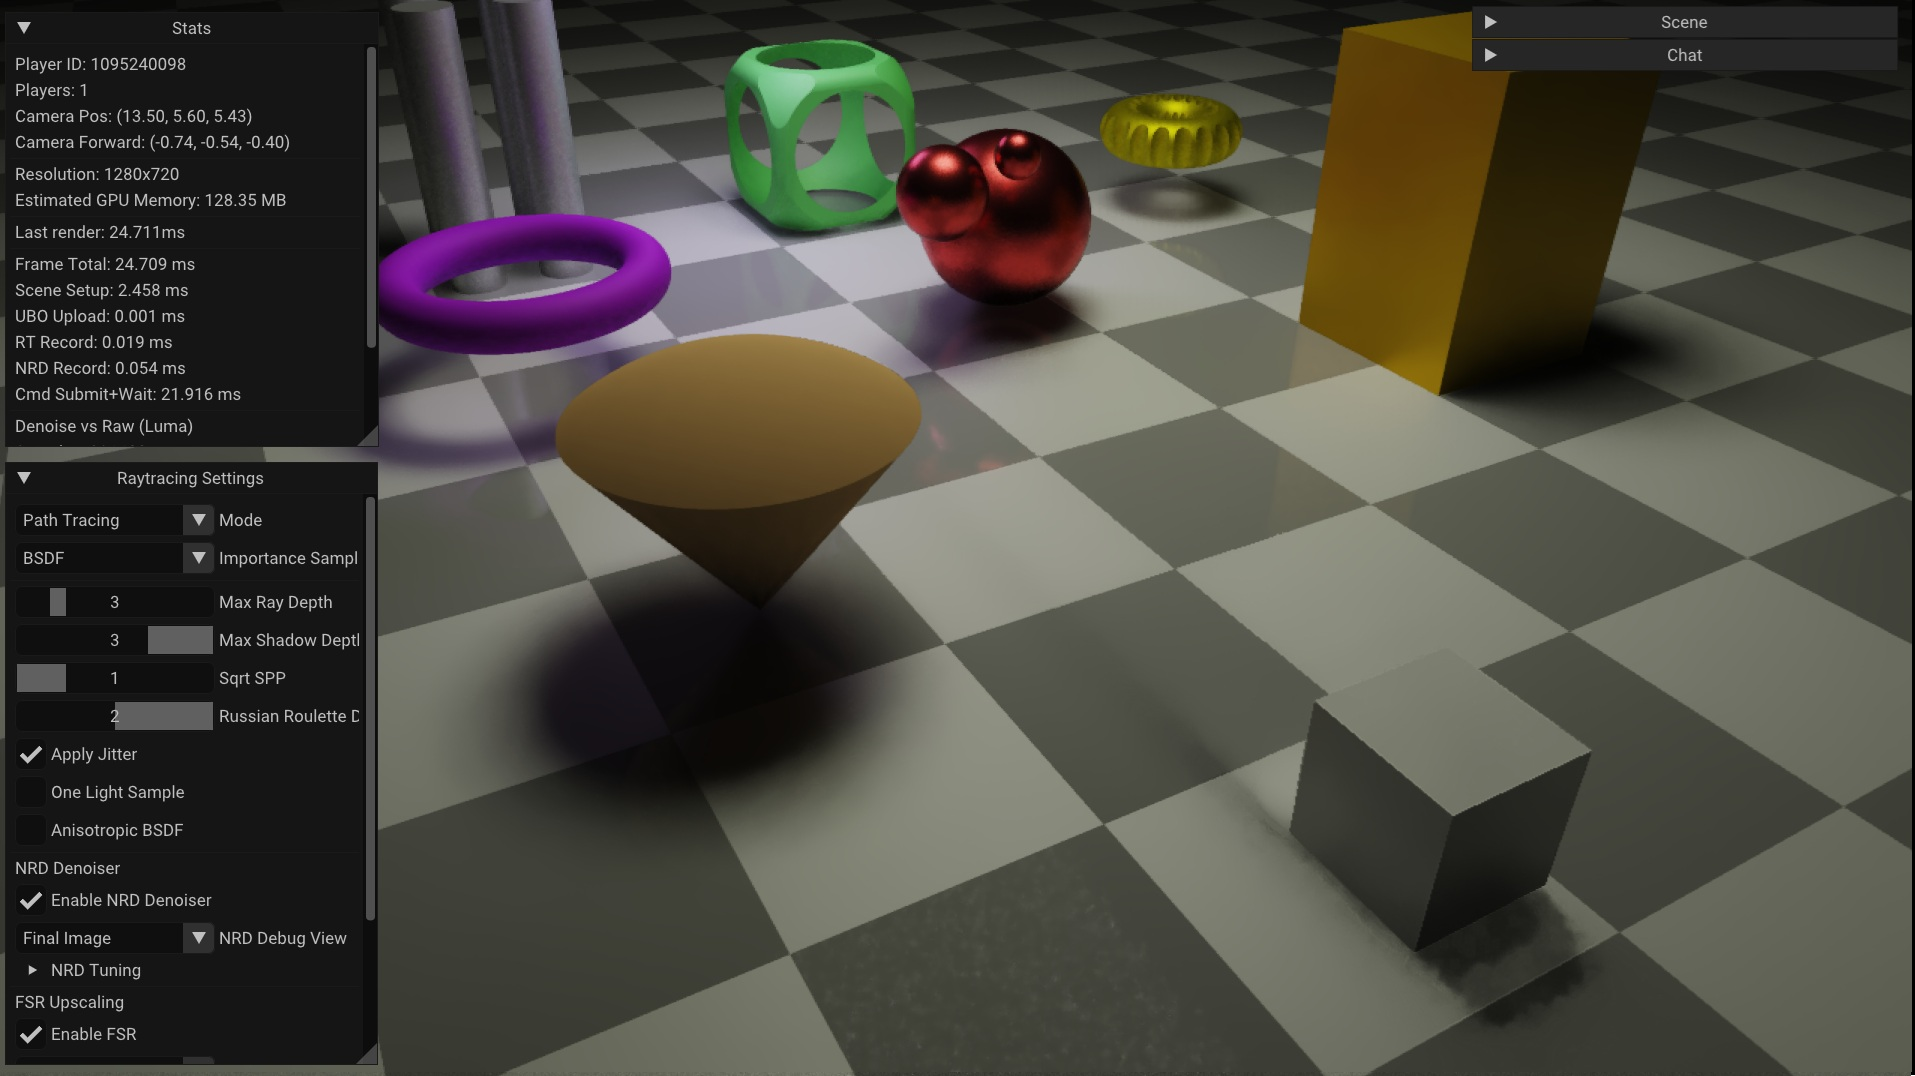
\includegraphics[width=\textwidth]{pics/demo-nrd-ghosting.jpg}
        \caption{NRD + FSR.}
    \end{subfigure}
    \hfill
    \begin{subfigure}[t]{0.32\textwidth}
        \centering
        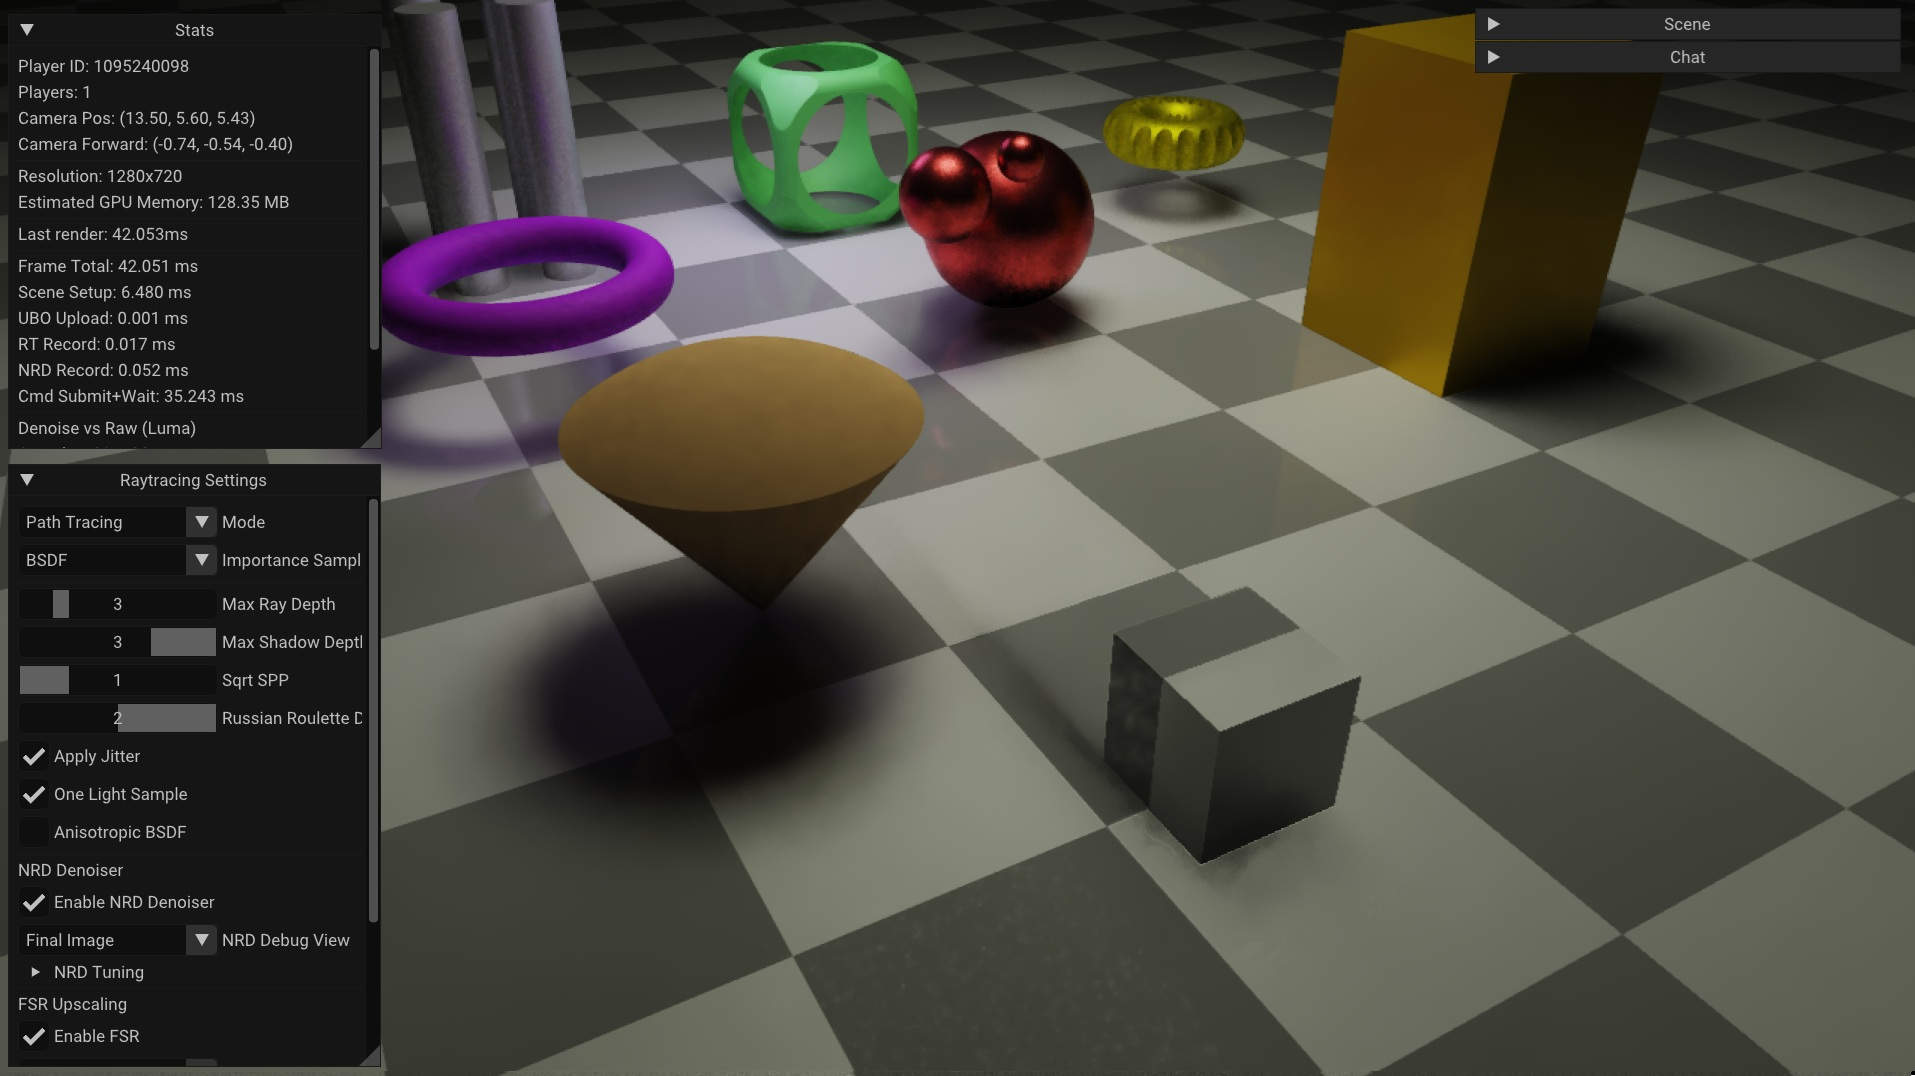
\includegraphics[width=\textwidth]{pics/demo-nrd-ols-shadow-ghosting.jpg}
        \caption{NRD + FSR + One Light Sample.}
    \end{subfigure}
    \caption{Exemple de ghosting în scena \texttt{demo} cu obiect în mișcare.}
    \label{fig:qual_demo_ghosting}
\end{figure}

\section{Evaluare cantitativă}

În continuare, vom evalua performanța aplicației în diferite scenarii, cu diferite setări de randare.
Pentru aceasta, am folosit un sistem cu următoarele specificații:

\begin{itemize}
    \item CPU: AMD Ryzen 5 5600H (6 nuclee, 12 fire de execuție)
    \item GPU: NVIDIA GeForce RTX 3060 Laptop GPU (TDP 130W, VRAM 6GB GDDR6, bus 192 bit, 3840 nuclee CUDA, 30 nuclee RT, 120 nuclee Tensor)
    \item RAM: 32GB DDR4 3200MT/s
    \item Sistem de operare: Windows 11 Pro
\end{itemize}

Majoritatea testelor (cu excepția celor la care menționez altfel) au fost efectuate în scena default Cornell Box, care se poate observa în Figura~\ref{fig:scene_editor}.
Setările default de randare sunt cele de mai jos:
\begin{itemize}
    \item Rezoluție de afișare: 1920x1080
    \item 1 spp
    \item NRD denoising off
    \item FSR upscaling off
    \item Max Ray Depth: 3
    \item Max Shadow Depth: 3
    \item Russian Roulette Depth: 3
\end{itemize}

Testarea s-a realizat cu un executabil compilat în modul \textit{Release}, cu flag-urile de optimizare uzuale activate.
Frametime-ul a fost capturat direct din fereastra de statistici (vezi Figura~\ref{fig:stats}).
Aceste metrici sunt capturate pe CPU, partea de lucru a GPU-ului fiind inclusă în totalitate în metrica \textit{Command Submit and Wait}.
Se afișează și o estimare a memoriei minime de care are nevoie GPU-ul pentru a rula scena, calculată ca suma memoriei necesare pentru geometrie, materiale, texturi și resurse de randare (imagini de output, buffer-e de scenă, SBT etc.).

Un ultim lucru de menționat este că partea de compute a GPU nu este saturată la maxim.
Modelul de dispatch este unul sincron, cu bariere explicite între etapele de RT, NRD și FSR, pentru a asigura corectitudinea vizuală și stabilitatea temporală.
De asemenea, din cauza integrărilor cu NRD și FSR, se prezintă un nivel ridicat de I/O CPU--GPU pentru actualizarea descriptorilor și a datelor de scenă, iar regiștrii din programele de shader sunt sub presiune, ceea ce poate limita performanța în anumite scenarii.

\begin{figure}[htb]
    \centering
    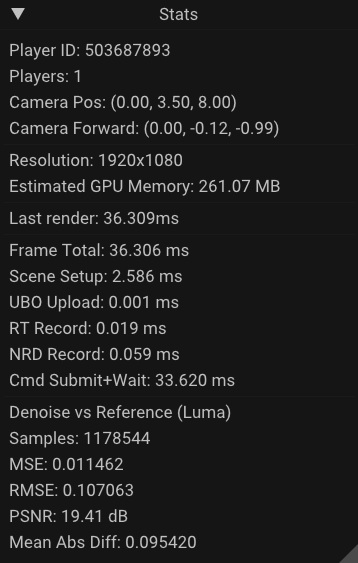
\includegraphics[width=0.4\textwidth]{pics/stats.jpg}
    \caption{Panoul de statistici, afișând frametime-ul și alte informații relevante.}
    \label{fig:stats}
\end{figure}

\begin{figure}[htb]
    \centering
    \begin{subfigure}[t]{0.49\textwidth}
        \centering
        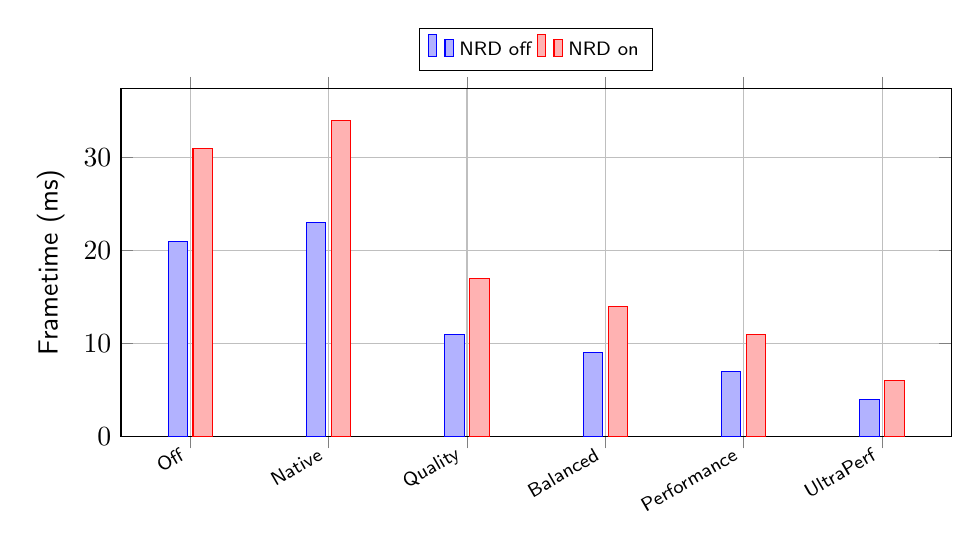
\begin{tikzpicture}
            \begin{axis}[
                ybar,
                bar width=7pt,
                width=\textwidth,
                height=6cm,
                ylabel={Frametime (ms)},
                symbolic x coords={Off,Native,Quality,Balanced,Performance,UltraPerf},
                xtick=data,
                x tick label style={rotate=30,anchor=east,font=\scriptsize},
                legend style={at={(0.5,1.05)},anchor=south,legend columns=2,font=\scriptsize},
                ymin=0,
                grid=major
            ]
                \addplot coordinates {(Off,21) (Native,23) (Quality,11) (Balanced,9) (Performance,7) (UltraPerf,4)};
                \addplot coordinates {(Off,31) (Native,34) (Quality,17) (Balanced,14) (Performance,11) (UltraPerf,6)};
                \legend{NRD off, NRD on}
            \end{axis}
        \end{tikzpicture}
        \caption{Frametime vs mod FSR}
    \end{subfigure}
    \hfill
    \begin{subfigure}[t]{0.49\textwidth}
        \centering
        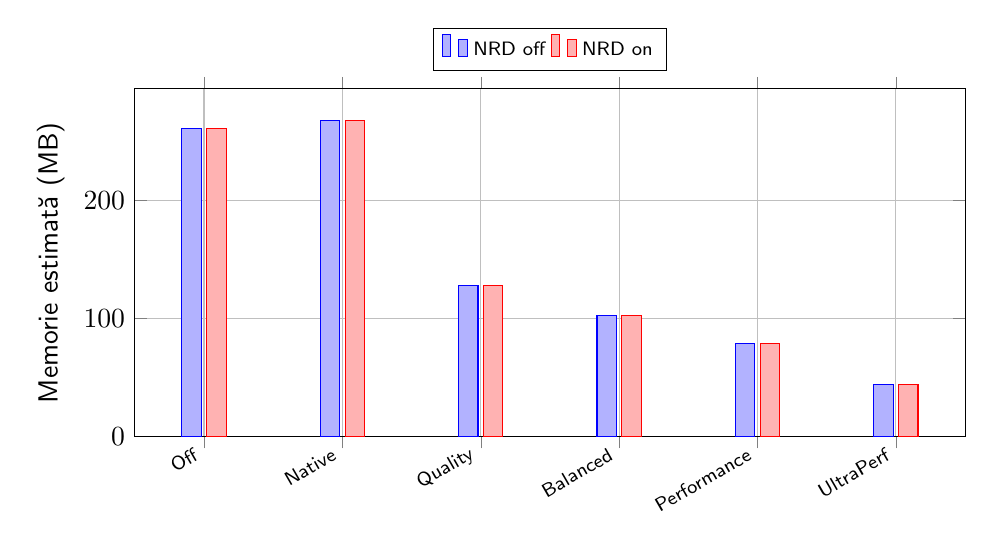
\begin{tikzpicture}
            \begin{axis}[
                ybar,
                bar width=7pt,
                width=\textwidth,
                height=6cm,
                ylabel={Memorie estimată (MB)},
                symbolic x coords={Off,Native,Quality,Balanced,Performance,UltraPerf},
                xtick=data,
                x tick label style={rotate=30,anchor=east,font=\scriptsize},
                legend style={at={(0.5,1.05)},anchor=south,legend columns=2,font=\scriptsize},
                ymin=0,
                grid=major
            ]
                \addplot coordinates {(Off,261) (Native,268) (Quality,128) (Balanced,103) (Performance,79) (UltraPerf,44)};
                \addplot coordinates {(Off,261) (Native,268) (Quality,128) (Balanced,103) (Performance,79) (UltraPerf,44)};
                \legend{NRD off, NRD on}
            \end{axis}
        \end{tikzpicture}
        \caption{Memorie vs mod FSR}
    \end{subfigure}
    \caption{Impactul modurilor FSR asupra frametime-ului și memoriei estimate.}
    \label{fig:eval_fsr}
\end{figure}

\begin{figure}[htb]
    \centering
    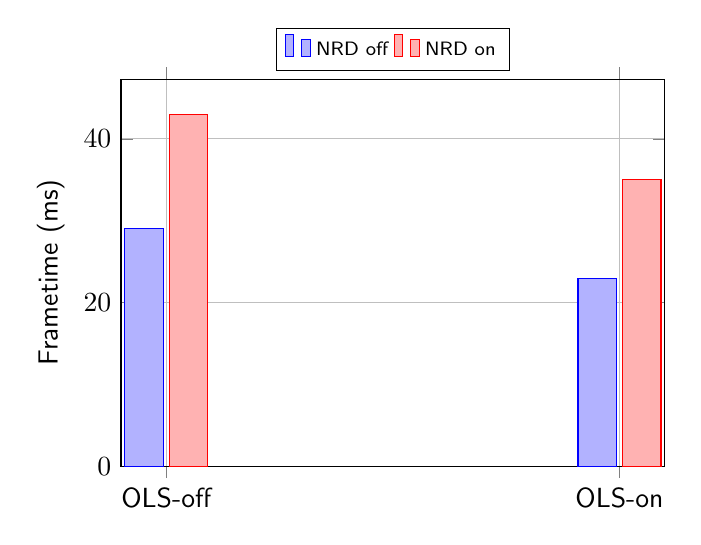
\begin{tikzpicture}
        \begin{axis}[
            ybar,
            bar width=14pt,
            width=0.7\textwidth,
            height=6.5cm,
            ylabel={Frametime (ms)},
            symbolic x coords={OLS-off,OLS-on},
            xtick=data,
            ymin=0,
            grid=major,
            legend style={at={(0.5,1.02)},anchor=south,legend columns=2,font=\scriptsize}
        ]
            \addplot coordinates {(OLS-off,29) (OLS-on,23)};
            \addplot coordinates {(OLS-off,43) (OLS-on,35)};
            \legend{NRD off, NRD on}
        \end{axis}
    \end{tikzpicture}
    \caption{Impactul \texttt{One Light Sample}: reducere de cost atât cu NRD dezactivat, cât și activat. Testul a fost făcut pe scena \texttt{demo}, cu două lumini de suprafață.}
    \label{fig:eval_ols}
\end{figure}

\begin{figure}[htb]
    \centering
    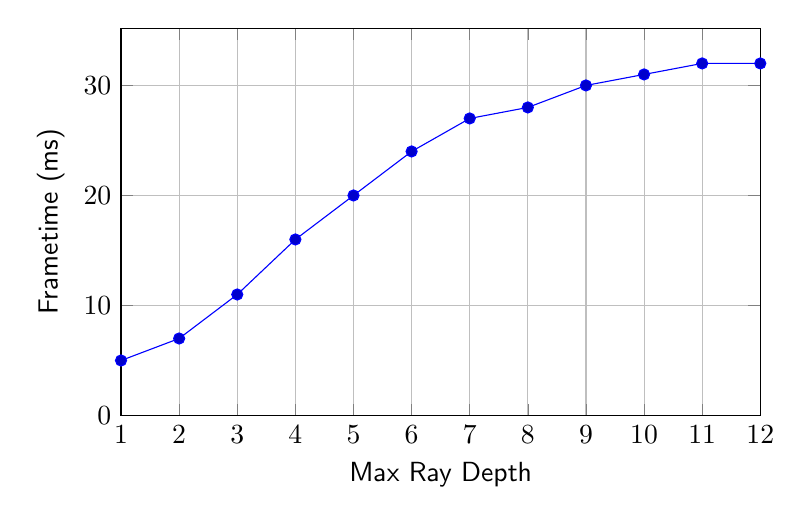
\begin{tikzpicture}
        \begin{axis}[
            width=0.8\textwidth,
            height=6.5cm,
            xlabel={Max Ray Depth},
            ylabel={Frametime (ms)},
            xmin=1, xmax=12,
            xtick={1,2,3,4,5,6,7,8,9,10,11,12},
            ymin=0,
            grid=major,
            mark=*]
            \addplot coordinates {(1,5) (2,7) (3,11) (4,16) (5,20) (6,24) (7,27) (8,28) (9,30) (10,31) (11,32) (12,32)};
        \end{axis}
    \end{tikzpicture}
    \caption{Scalarea costului de randare în funcție de \texttt{Max Ray Depth} (\texttt{Max Shadow Depth = 1}).}
    \label{fig:eval_ray_depth}
\end{figure}

\begin{figure}[htb]
    \centering
    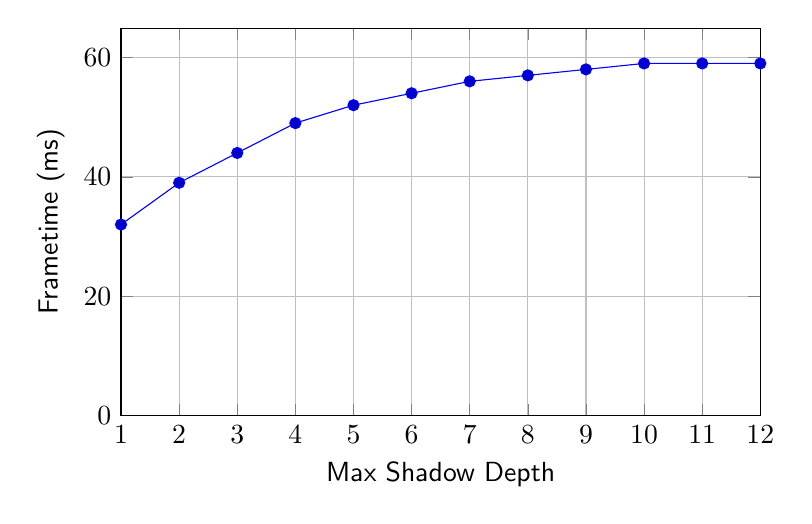
\begin{tikzpicture}
        \begin{axis}[
            width=0.8\textwidth,
            height=6.5cm,
            xlabel={Max Shadow Depth},
            ylabel={Frametime (ms)},
            xmin=1, xmax=12,
            xtick={1,2,3,4,5,6,7,8,9,10,11,12},
            ymin=0,
            grid=major,
            mark=*]
            \addplot coordinates {(1,32) (2,39) (3,44) (4,49) (5,52) (6,54) (7,56) (8,57) (9,58) (10,59) (11,59) (12,59)};
        \end{axis}
    \end{tikzpicture}
    \caption{Scalarea costului de randare în funcție de \texttt{Max Shadow Depth} (\texttt{Max Ray Depth = 12}).}
    \label{fig:eval_shadow_depth}
\end{figure}

\begin{figure}[htb]
    \centering
    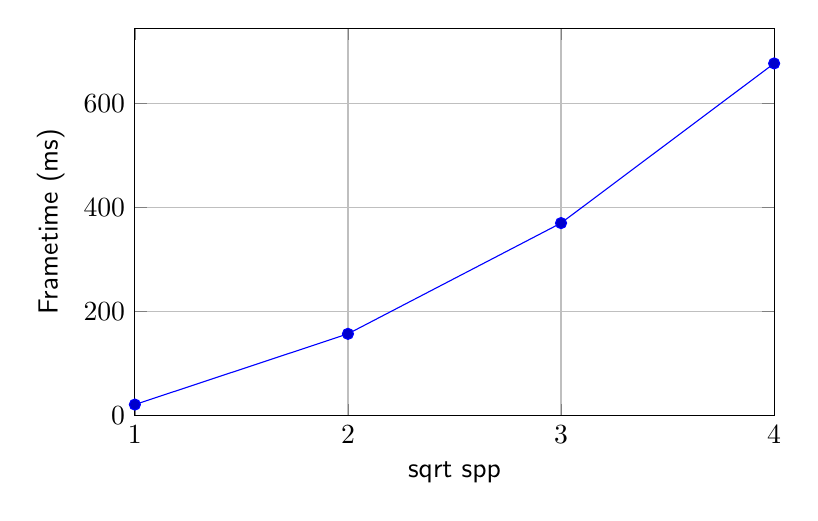
\begin{tikzpicture}
        \begin{axis}[
            width=0.8\textwidth,
            height=6.5cm,
            xlabel={sqrt spp},
            ylabel={Frametime (ms)},
            xmin=1, xmax=4,
            xtick={1,2,3,4},
            ymin=0,
            grid=major,
            mark=*]
            \addplot coordinates {(1,21) (2,157) (3,370) (4,677)};
        \end{axis}
    \end{tikzpicture}
    \caption{Creșterea costului de randare în funcție de \texttt{sqrt spp}.}
    \label{fig:eval_sqrt_spp}
\end{figure}

\begin{figure}[htb]
    \centering
    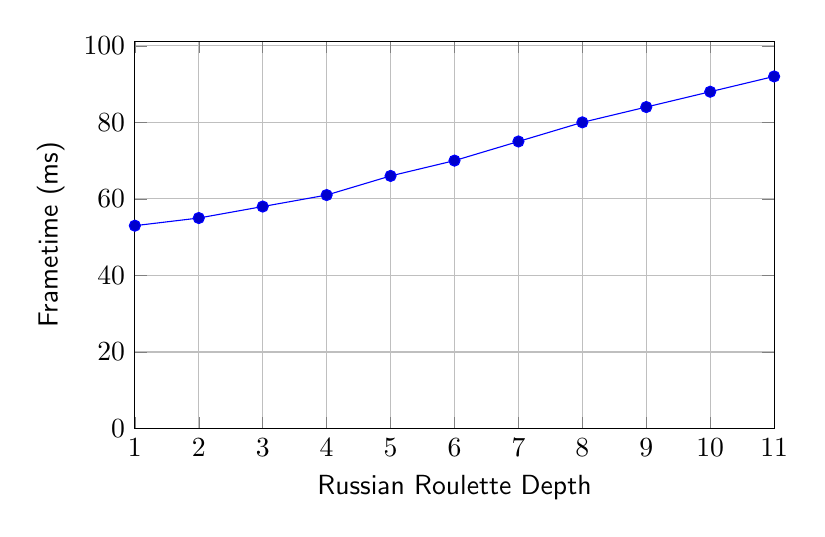
\begin{tikzpicture}
        \begin{axis}[
            width=0.8\textwidth,
            height=6.5cm,
            xlabel={Russian Roulette Depth},
            ylabel={Frametime (ms)},
            xmin=1, xmax=11,
            xtick={1,2,3,4,5,6,7,8,9,10,11},
            ymin=0,
            grid=major,
            mark=*]
            \addplot coordinates {(1,53) (2,55) (3,58) (4,61) (5,66) (6,70) (7,75) (8,80) (9,84) (10,88) (11,92)};
        \end{axis}
    \end{tikzpicture}
    \caption{Impactul pragului de start \texttt{Russian Roulette Depth} asupra costului de randare (\texttt{Max Ray Depth = 12}, \texttt{Max Shadow Depth = 12}).}
    \label{fig:eval_rr_depth}
\end{figure}


Datele confirmă un compromis clar între fidelitate și cost computațional.
FSR upscaling reduce semnificativ frametime-ul pe măsură ce scade rezoluția internă, concomitent cu reducerea memoriei estimate (datorită randării la o rezoluție internă mai mică).
Activarea NRD adaugă un cost relativ stabil peste fiecare mod FSR, dar rămâne compatibilă cu scenarii interactive în modurile \textit{Quality/Balanced}.
Curbele pentru \texttt{Max Ray Depth} și \texttt{Max Shadow Depth} indică o zonă de saturație: după un anumit prag, costul crește mai lent (datorită efectului de ruletă rusească), în timp ce câștigul vizual tinde să fie marginal.
În schimb, creșterea \texttt{sqrt spp} are impact super-liniar asupra frametime-ului, fiind cel mai scump parametru dintre cei evaluați.
Curba pentru \texttt{Russian Roulette Depth} este aproape liniară în intervalul testat: cu cât întârziem activarea ruletei rusești, cu atât mai multe bounce-uri complete sunt evaluate și costul total crește.
În final, \texttt{One Light Sample} oferă un câștig de performanță consistent, dezlegând costul computațional de configurația de lumini din scenă.
Totuși, sugerăm ca această setare să fie activată în tandem cu NRD, pentru a compensa zgomotul rezidual și a păstra stabilitatea temporală.

Recomandarea noastră, având în vedere analizele calitative și cantitative, este de a folosi următoarele setări:

\begin{itemize}
    \item NRD activat, cu parametrii default.
    \item FSR activat în modurile \textit{Quality} sau \textit{Balanced}, în funcție de puterea de procesare.
          Dacă aceasta permite, modul de antialiasing \textit{Native} este o alternativă bună la algoritmi precum TAA sau MSAA.
    \item \texttt{One Light Sample} activat pentru scenarii cu mai multe lumini.
    \item \texttt{Max Ray Depth} și \texttt{Max Shadow Depth} setate la 3-4.
          \texttt{Max Shadow Depth} este bine în general să fie egal cu \texttt{Max Ray Depth}, pentru a evita situațiile în care bounce-urile adânci nu pot genera raze de umbră, ceea ce duce la artefacte vizuale.
    \item \texttt{sqrt spp} setat la 1. Orice valoare peste 1 distruge interactivitatea aplicației.
    \item \texttt{Russian Roulette Depth} să fie setată la un prag mic, eventual maxim 3-4.
\end{itemize} 


\chapter{\label{sec:concluzii}Concluzii}

Lucrarea de față reprezintă realizarea obiectivului principal de a porta și extinde motorul de Ray Tracing \texttt{DieXaR}~\cite{DieXaR2024} către un ecosistem modern, portabil și orientat către dezvoltare practică.
Rezultatul este \texttt{Vlkrt}, un motor grafic bazat pe Vulkan, care păstrează fundația algoritmică din proiectul anterior, dar adaugă o arhitectură mai robustă și un set de funcționalități relevante pentru un produs real: editor de scene, scripting, arhitectură client-server, denoising, upscaling, precum și instrumente de evaluare vizuală și cantitativă.

Din punct de vedere tehnic, realizarea majoră este demonstrarea faptului că un pipeline de Ray Tracing care rezolvă ecuația de iluminare~(\ref{eq:light_transport}) poate fi adus într-un regim interactiv pe hardware consumer, cu rezultate satisfăcătoare la nivel de calitate a imaginii.
Dacă scopul inițial al \texttt{DieXaR} a fost de a demonstra la nivel brut tehnologia, \texttt{Vlkrt} o șlefuiește și o aduce într-un format cât mai aproape de un prototip extensibil, pe care se poate construi un motor grafic de producție.

În mod realist, proiectul are și limitări.
În primul rând, calitatea imaginii variază de la o scenă la alta.
Dacă nu există lumini direcționale care să domine contribuția energetică, imaginea de bază conține mult zgomot la 1 spp.
Algoritmul de denoising ajută mult la reducerea acestui zgomot, însă componenta temporală are de suferit în aceste situații.
De asemenea, nici denoiser-ul și nici upscaler-ul nu implementează algoritmi bazați pe AI -- ceea ce reprezintă un dezavantaj în industria curentă.
O altă limitare ține de scalabilitate: structurile de accelerație sunt reconstruite în mod conservator la modificări, și nu împart scena în mod optim între obiecte dinamice și \textit{prop-uri} statice.

Aceste limitări definesc, de fapt, direcțiile cele mai valoroase pentru continuarea lucrării.
În prim plan, adăugarea de suport pentru metode din sfera de \textit{Neural Rendering} vor aduce acest motor și mai aproape de producție.
În plan secund, o gestionare mai generică de scene (suport pentru formate arbitrare), materiale și organizare a structurilor de accelerare sunt necesare pentru a putea scala către lumi masive cum ar fi cele din genul \textit{Open World}.

O concluzie practică a cercetării efectuate în cadrul acestei lucrări este că valoarea unui motor de Ray Tracing nu este dată doar de rezultate, ci mai ales de capacitatea sa de a fi instrument de învățare și experimentare.
Am petrecut mult timp schimbând parametri, experimentând cu optimizări, adâncindu-mă în branch-uri pe care le-am abandonat în final, și am învățat multe din acest proces.
Sunt destul de mulțumit cu rezultatul final, însă întotdeauna este loc de îmbunătățiri.


\bibliographystyle{plain}
\bibliography{bibliography}

\chapter*{Anexe}\addcontentsline{toc}{chapter}{Anexe}

\begin{appendices}\label{anexa}

\chapter{Figuri}

\begin{figure}[htb]
	\centering
	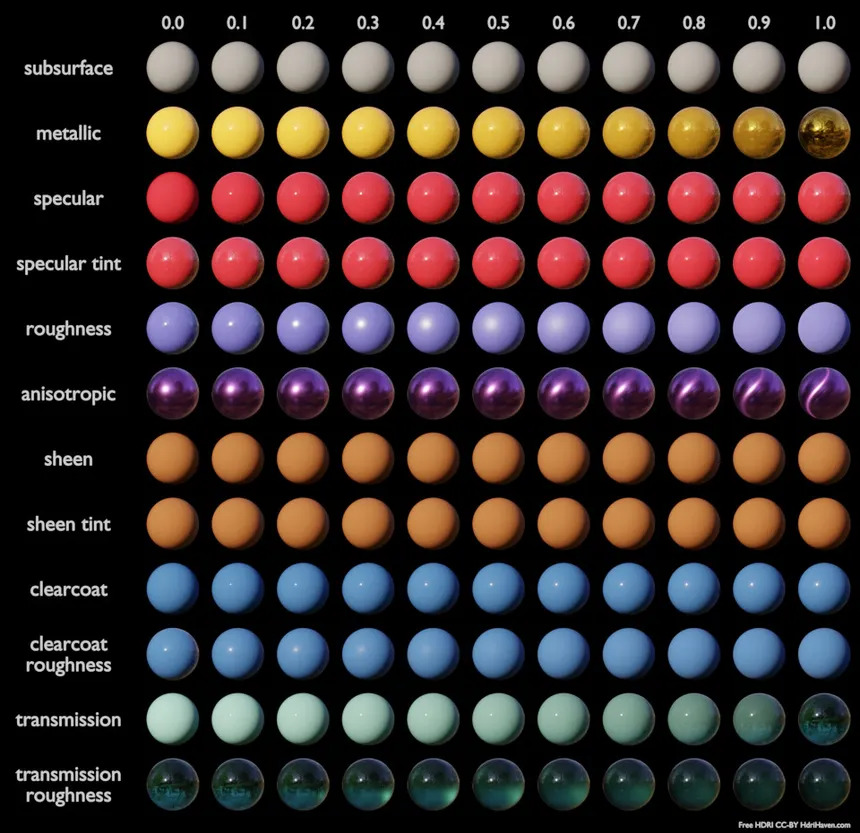
\includegraphics[width=\textwidth]{pics/disney-bsdf.jpg}
	\caption{Parametrii modelului Disney Principled BSDF~\cite{DisneyBSDF}.\protect\footnotemark}
	\label{fig:disney_params}
\end{figure}
\footnotetext{\copyright\url{https://docs.blender.org/manual/en/3.2/render/shader_nodes/shader/principled.html}. Accesat 13.06.2026.}

\begin{figure}[htb]
    \centering
    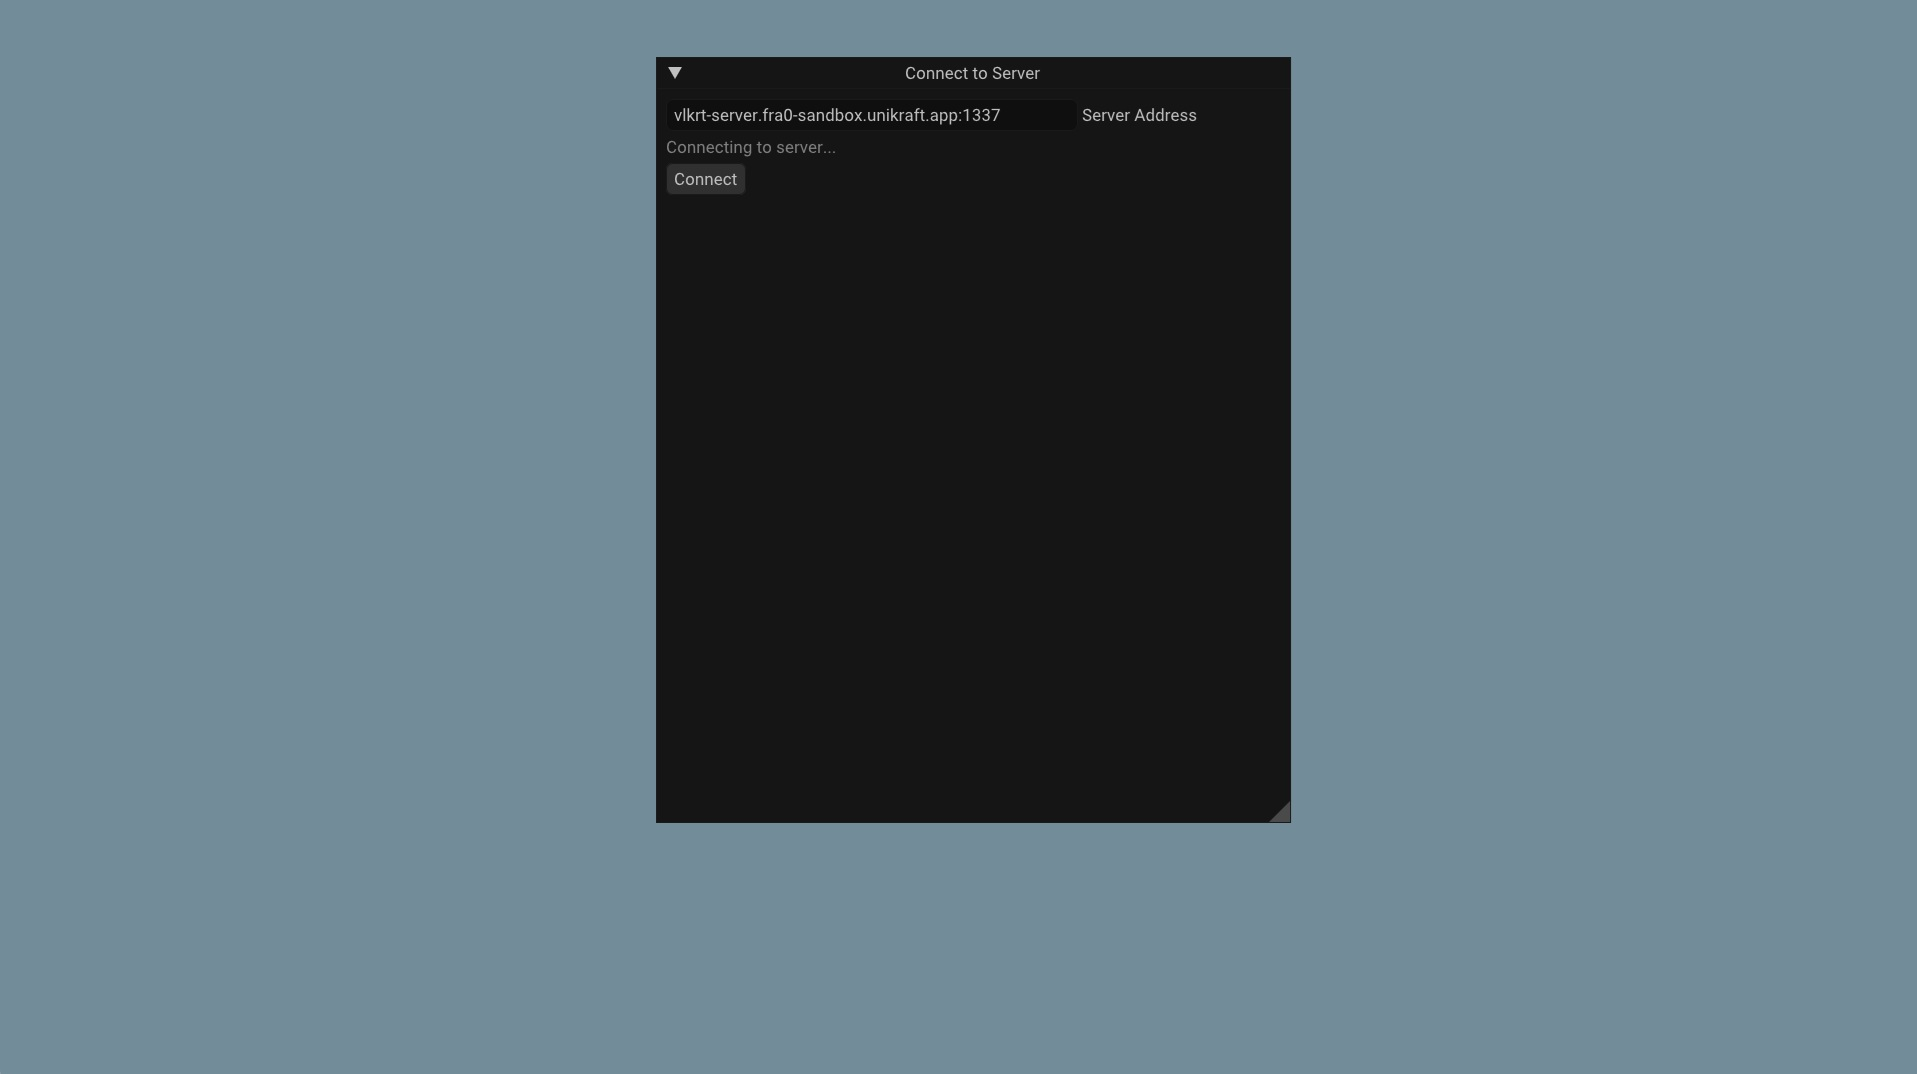
\includegraphics[width=\textwidth]{pics/conectare-server.jpg}
    \caption{Meniul de conectare la server, unde utilizatorul poate introduce adresa și portul pentru conexiune. În acest caz, serverul este deployat pe platforma Unikraft Cloud\footref{ftn:unikraft}.}
    \label{fig:conectare_server}
\end{figure}

\begin{figure}[htb]
    \centering
    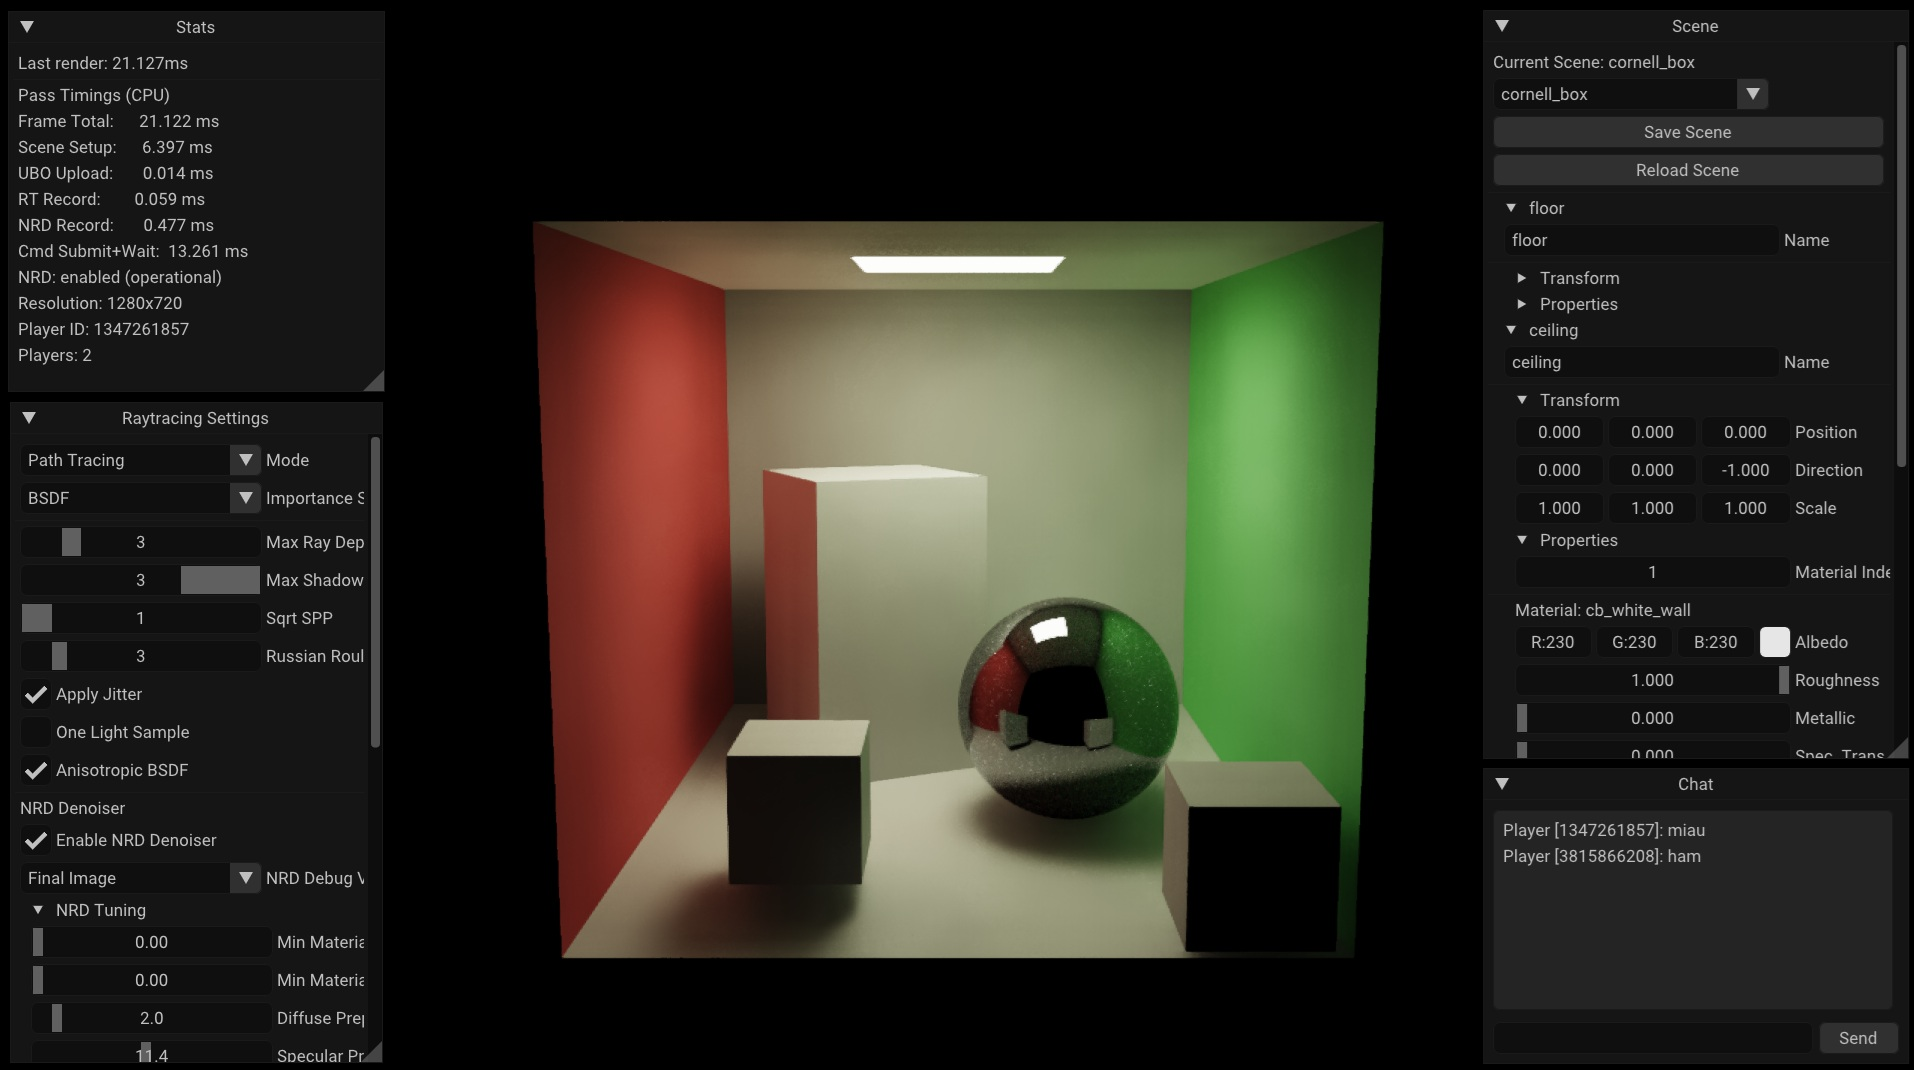
\includegraphics[width=\textwidth]{pics/vlkrt-ansamblu.jpg}
    \caption{Privire de ansamblu asupra aplicației \texttt{Vlkrt}. În scenă se pot observa obiecte statice, precum și avatarii jucătorilor conectați (cele două cuburi). Se pot observa, în ordine trigonometrică, editorul de scene, panoul de statistici, panoul de setări grafice și fereastra de chat.}
    \label{fig:vlkrt_ansamblu}
\end{figure}

\chapter{Extrase de cod}

\begin{algorithm}[H]
	\caption{Pseudocodul algoritmului de Path Tracing recursiv, extras din~\cite{DieXaR2024}.}\label{alg:path_tracing}
	\begin{algorithmic}[1]
		\Function{PathTrace}{$ray, depth$}
		\If{$depth > MAX\_DEPTH$}
		\State \Return $backgroundColor$	\Comment{Ne oprim dacă am atins adâncimea maximă}
		\EndIf
		\State $intersection \gets$ \Call{IntersectScene}{$ray$} \Comment{Intersectăm raza cu scena}
		\If{$intersection = \texttt{null}$}
		\State \Return $backgroundColor$	\Comment{Ne oprim dacă nu există intersecție}
		\EndIf
		\State $m \gets intersection.material$
		\State $p \gets intersection.position$
		\State $n \gets intersection.normal$
		\State $v \gets -ray.direction$
		\State $bounceRay \gets$ \Call{SampleRay}{$m, p, n$}	\Comment{Eșantionăm o nouă rază}
		\State $pdf \gets$ \Call{Pdf}{$m, n, bounceRay$}		\Comment{Evaluăm probabilitatea de eșantionare}
		\State $reflectance \gets$ \Call{EvalBRDF}{$m, n, v, bounceRay$} \Comment{Evaluăm reflectanța}
		\State $color \gets$ \Call{PathTrace}{$bounceRay, depth + 1$}	 \Comment{Pasul recursiv}
		\State \Return $m.emission + reflectance \cdot color / pdf$		 \Comment{Evaluăm ecuația de rendering}
		\EndFunction
		\Function{Render}{$pixels, samples$}
		\For {$p$ in $pixels$}
		\For {$i \gets 1$ to $samples$}
		\State $ray \gets$ \Call{GenerateCameraRay}{$p, i$}	\Comment{Generăm raza de la observator}
		\State $pixel.color \gets pixel.color + $ \Call{PathTrace}{$ray, 0$}	\Comment{Acumulăm contribuția}
		\EndFor
		\State $pixel.color \gets pixel.color / samples$ \Comment{Mediem contribuțiile}
		\EndFor
		\EndFunction
	\end{algorithmic}
\end{algorithm}

\begin{lstlisting}[caption={Structură pentru materiale BSDF, cu suport pentru texturi albedo.}, language=C++, label={lst:material_structures}, frame=single]
struct Material
{
	std::string Name;
	glm::vec3 Albedo{ 1.0f };     // Culoarea de baza a materialului
	glm::vec3 Emission{ 0.0f };   // Culoarea emisiei (pentru materiale emisive)
	glm::vec3 Extinction{ 1.0f }; // Culoarea absorbtiei luminii in material
	float AtDistance{ 1.0f };     // Distanta la care lumina este redusa la 1/e din intensitatea sa originala (pentru materiale transparente)
	float Roughness{ 0.5f };      // Netezimea suprafetei
	float Metallic{ 0.0f };       // Gradul de metalicitate (0 = dielectric, 1 = metal)
	float Subsurface{ 0.0f };     // Gradul de subsurface scattering (0 = fara SSS, 1 = maxim SSS)
	float Anisotropic{ 0.0f };    // Gradul de anisotropie (0 = isotropic, 1 = maxim anisotropic)
	float Sheen{ 0.0f };          // Intensitatea efectului de sheen (retroreflexie, specifica materialelor textile)
	float SheenTint{ 0.5f };      // Tenta pentru efectul de sheen (0 = alb, 1 = culoarea albedo)
	float Clearcoat{ 0.0f };      // Intensitatea stratului de clearcoat (0 = fara clearcoat, 1 = clearcoat complet)
	float ClearcoatGloss{ 1.0f }; // Netezimea stratului de clearcoat (0 = mat, 1 = lucios)
	float SpecularTint{ 0.0f };   // Tenta pentru componenta speculara (0 = alb, 1 = culoarea albedo)
	float SpecularTransmission{ 0.0f }; // Gradul de transmisie speculara (0 = fara transmisie, 1 = transmisie completa)
	float Eta{ 1.5f }; // Indicele de refractie
	float StepScale{ 1.0f };  // Factor de scalare pentru Ray Marching (pentru SDF-uri)
	uint32_t MaterialIndex{ 0 };
	int32_t LightIndex{ -1 };
	std::string TextureFilename;
	float Tiling{ 1.0f };  // Factor de tiling pentru textura
};
\end{lstlisting}

\begin{lstlisting}[caption={Exemplu de scenă reprezentată în format YAML.}, label={lst:scene_example}, frame=single]
materials:
- name: stone
  albedo: [ 0.5, 0.5, 0.5 ]
  roughness: 0.8
  metallic: 0.1
  texture: tiles.jpg
  tiling: 5
  material_index: 0
- name: metal
  albedo: [ 0.8, 0.8, 0.8 ]
  roughness: 0.2
  metallic: 1
  texture: wood.jpg
  tiling: 0.5
  material_index: 0
- name: bricks
  albedo: [ 0.9, 0.9, 0.9 ]
  roughness: 0.9375
  metallic: 0.1
  texture: brick.jpg
  tiling: 2
  material_index: 0

entities:
- name: scene_root
  type: empty
  transform:
    position: [ 0, -0.408099, 0 ]
    rotation: [ 0, 0, 0, 0 ]
    scale: [ 1, 1, 1 ]
  children:
  - name: grounded
    type: mesh
    transform:
      position: [ 0, -1, 0 ]
      rotation: [ 0, 0, 0, 1 ]
      scale: [ 10, 1, 10 ]
    mesh: ground.obj
    material: 0
  - name: cube
    script: cube_animation.lua
    type: mesh
    transform:
      position: [ 2, -0.180116, 0 ]
      rotation: [ -0, -0.776384, -0, -0.630261 ]
      scale: [ 1, 1, 1 ]
    mesh: cube.obj
    material: 1
  - name: lighting_group
    type: empty
    transform:
      position: [ -0.909, 5, 5 ]
      rotation: [ -0.643505, 0.0327726, 0, 0.76474 ]
      scale: [ 3.61, 1, 1 ]
    children:
    - name: point
      type: light
      transform:
        position: [ 2.9, 0, 0 ]
        rotation: [ 0, 0, 0, 1 ]
        scale: [ 1, 1, 1 ]
      light_emission: [ 1, 1, 1 ]
      light_intensity: 1.5
      light_type: 0
      light_direction: [ 0, 0, -1 ]
      light_size: 1.825
    - name: sun
      type: light
      transform:
        position: [ 0, 0, 0 ]
        rotation: [ 0.288279, -0.0836488, 0, 0.953886 ]
        scale: [ 1, 1, 1 ]
      light_emission: [ 0.729107, 0.518529, 0.275254 ]
      light_intensity: 1.798
      light_type: 1
      light_direction: [ 0.159583, 0.54997, -0.819797 ]

scene_settings:
  background_color: [ 0, 0, 0 ]
  scene_index: 0
  max_recursion_depth: 4
  max_shadow_recursion_depth: 4
  path_sqrt_samples: 1
  russian_roulette_depth: 3
  apply_jitter: true
  anisotropic_bsdf: true
  enable_fsr: false
  fsr_quality_mode: 1
  fsr_sharpness: 0
\end{lstlisting}

\begin{lstlisting}[caption={Structură pentru parametrii de denoising NRD.}, language=C++, label={lst:nrd_params}, frame=single]
struct NRDDenoiseParams
{
    uint32_t FrameIndex{ 0 };
    uint32_t Width{ 0 };
    uint32_t Height{ 0 };

    // Matrices are column-major
    float ViewToClip[16]{};
    float ViewToClipPrev[16]{};
    float WorldToView[16]{};
    float WorldToViewPrev[16]{};

    float CameraJitter[2]{ 0.0f, 0.0f };
    float CameraJitterPrev[2]{ 0.0f, 0.0f };

    // Runtime RELAX tuning (can be updated from GUI)
    float MinMaterialForDiffuse{ 0.0f };
    float MinMaterialForSpecular{ 0.0f };
    float DiffusePrepassBlurRadius{ 6.0f };
    float SpecularPrepassBlurRadius{ 10.0f };
    uint32_t DiffuseMaxAccumulatedFrameNum{ 10 };
    uint32_t SpecularMaxAccumulatedFrameNum{ 12 };
    uint32_t DiffuseMaxFastAccumulatedFrameNum{ 2 };
    uint32_t SpecularMaxFastAccumulatedFrameNum{ 3 };
    float AntilagAccelerationAmount{ 0.9f };
    float AntilagSpatialSigmaScale{ 2.5f };
    float AntilagTemporalSigmaScale{ 0.22f };
    float AntilagResetAmount{ 1.0f };
    float DisocclusionThreshold{ 0.010f };
    float DisocclusionThresholdAlternate{ 0.035f };

    bool HasValidMatrices = false;
};
\end{lstlisting}

\end{appendices}
\end{document}